\documentclass[a4paper]{report}

% Packages
\usepackage[nodisplayskipstretch]{setspace} % must be before algorithm & float
\usepackage[noend]{algpseudocode}
\usepackage[textformat=period]{caption}
\usepackage[hidelinks]{hyperref}
\usepackage[UKenglish]{isodate}
\usepackage[refpage, intoc]{nomencl}
\usepackage[nottoc]{tocbibind}
\usepackage{algorithm}
\usepackage{aliascnt}
\usepackage{amsfonts}
\usepackage{amsmath}
\usepackage{amssymb}
\usepackage{amsthm}
\usepackage{array}
\usepackage{cancel}
\usepackage{colortbl}
\usepackage{dot2texi}
\usepackage{draftwatermark}
\usepackage{enumerate}
\usepackage{float}
\usepackage{forest}
\usepackage{lipsum}
\usepackage{longtable}
\usepackage{makeidx}
\usepackage{mathdots}
\usepackage{mathrsfs}
\usepackage{mathtools}
\usepackage{multicol}
\usepackage{multirow}
\usepackage{pifont}
\usepackage{pstricks}
%\usepackage{showframe}
\usepackage{svg}
\usepackage{tikz-cd}
\usepackage{tikz}
\usepackage{url}
\usepackage{xcolor}
\usepackage{xfrac}

% List of notation
\renewcommand\nomname{List of notation}
\def\pagedeclaration#1{\dotfill \hyperlink{page.#1}{\nobreakspace#1}}

% Compile the index and notation
\makeindex
\makenomenclature

% Automatic bracket sizing
%\usepackage{nath}
%\delimgrowth=1
%\delimitershortfall=-1pt

% Other library imports
\usetikzlibrary{arrows,shapes}
\forestset{uf/.style={for tree={edge={<-}}}}

% Algorithmic
\algnewcommand\algorithmicbreak{\textbf{break}}
\algnewcommand\Break{\algorithmicbreak{} }

% Hyperlink references (invisible)
%\hypersetup{linkcolor=black, urlcolor=black, citecolor=black}

% Fix double spacing in arrays
\setlength{\jot}{-1ex}
\renewcommand*\arraystretch{.7}

% Watermark with git hash
\immediate\write18{git rev-parse --short HEAD > hash.info}
\immediate\write18{git diff --shortstat > changes.info}
\immediate\write18{git diff --staged --shortstat >> changes.info}
\SetWatermarkText{Commit \input{hash.info} \quad \input{changes.info}}
\SetWatermarkColor[gray]{0.75}
\SetWatermarkFontSize{0.5cm}
\SetWatermarkAngle{90}
\SetWatermarkHorCenter{3cm}

% Macros
% Text operators
\DeclareMathOperator\rank{rank}
\DeclareMathOperator\Cong{Cong}
\DeclareMathOperator\id{id}
\DeclareMathOperator\im{im}
\DeclareMathOperator\tr{tr}
\DeclareMathOperator\dom{dom}
\DeclareMathOperator\codom{codom}
\DeclareMathOperator\coker{coker}

% Green's relations
\newcommand{\HH}{\mathrel{\mathscr{H}}}
\newcommand{\LL}{\mathrel{\mathscr{L}}}
\newcommand{\RR}{\mathrel{\mathscr{R}}}
\newcommand{\DD}{\mathrel{\mathscr{D}}}
\newcommand{\JJ}{\mathrel{\mathscr{J}}}

\newcommand{\nHH}{\mathrel{\cancel{\mathscr{H}}}}
\newcommand{\nLL}{\mathrel{\cancel{\mathscr{L}}}}
\newcommand{\nRR}{\mathrel{\cancel{\mathscr{R}}}}
\newcommand{\nDD}{\mathrel{\cancel{\mathscr{D}}}}
\newcommand{\nJJ}{\mathrel{\cancel{\mathscr{J}}}}

% Other relations
\newcommand{\sS}{\mathcal{S}}
\newcommand{\tT}{\mathcal{T}}
\newcommand{\R}{\mathbf{R}}
\newcommand{\Rs}{\mathbf{R}^\sharp}

% Special semigroups
\newcommand{\T}{\mathcal{T}}
\newcommand{\I}{\mathcal{I}}
\newcommand{\OO}{\mathcal{O}}
\newcommand{\LZ}{\mathcal{L\!Z}}
\newcommand{\RZ}{\mathcal{R\!Z}}
\newcommand{\Z}{\mathcal{Z}}
\newcommand{\PBR}{\mathcal{P}\!B}
\newcommand{\PT}{\mathcal{P\!T}}
\newcommand{\Sym}{\mathcal{S}}
\newcommand{\Alt}{\mathcal{A}}
\newcommand{\Mot}{\mathcal{M}}
\newcommand{\Prt}{\mathcal{P}}

% Other little shortcuts
\newcommand{\bn}{\mathbf{n}}

% Rewriting systems
\newcommand{\rws}{\mathbf{R}}
\newcommand{\tostar}{\stackrel{*}{\to}}
\newcommand{\lrstar}{\stackrel{*}{\leftrightarrow}}

% Double angle brackets
\newcommand{\llangle}{\langle\!\langle}
\newcommand{\rrangle}{\rangle\!\rangle}

% Ticks and crosses
\newcommand{\cmark}{\ding{51}}
\newcommand{\xmark}{\ding{56}}

% Algorithmicx
\algnewcommand\True{\textbf{true}\space}
\algnewcommand\False{\textbf{false}\space}
\algnewcommand{\LComment}[1]{\State \(\triangleright\) \emph{#1}}
\algnewcommand{\Or}{~\textbf{or}~}
\algnewcommand{\And}{~\textbf{and}~}
\algnewcommand{\Continue}{\textbf{continue}}

% Transformations
\newcommand{\transII}[2]{
\begin{pmatrix}
  1 & 2 \\
  #1 & #2
\end{pmatrix}
}
\newcommand{\transV}[5]{
\begin{pmatrix}
  1 & 2 & 3 & 4 & 5 \\
  #1 & #2 & #3 & #4 & #5
\end{pmatrix}
}

% Presentations
\newcommand{\pres}[2]{\left\langle\,#1 ~\middle|~ #2\,\right\rangle}

% Todd-Coxeter tables with 2 generators
\newcommand{\tctableAB}[4]{
\begin{table}[H]
  \centering
  \begin{tabular}{c | c | c |}
    \multicolumn{1}{c}{} &
    \multicolumn{1}{c}{$a$} &
    \multicolumn{1}{c}{$b$} \\
    \cline{2-3}
    #4
    \cline{2-3}
  \end{tabular}
  \caption[#2]{#3}
  \label{#1}
\end{table}
}

% Partition diagrams
% \tikzset{>=latex}
\newcommand{\bipartdiagscale}{.36}
\newcommand{\tv}[2]{ % Transversal line
  \draw(#1,2)--(#2,0);
}
\newcommand{\tc}[2]{ % Top curve
  \draw(#1, 1.875) .. controls (#1, 1.5) and (#2, 1.5) .. (#2, 1.875);
}
\newcommand{\bc}[2]{ % Bottom curve
  \draw(#1, 0.125) .. controls (#1, 0.5) and (#2, 0.5) .. (#2, 0.125);
}
\newcommand{\bC}[2]{ % Bottom curve (bigger)
  \draw(#1, 0.125) .. controls (#1, 0.75) and (#2, 0.75) .. (#2, 0.125);
}
\newcommand{\utv}[2]{ % Transversal (upper diagram)
  \draw(#1,4)--(#2,2);
}
\newcommand{\utc}[2]{ % Top curve (upper diagram)
  \draw(#1, 3.875) .. controls (#1, 3.5) and (#2, 3.5) .. (#2, 3.875);
}
\newcommand{\ubc}[2]{ % Bottom curve (upper diagram)
  \draw(#1, 2.125) .. controls (#1, 2.5) and (#2, 2.5) .. (#2, 2.125);
}

\newcommand{\trans}[5]{ % Transformation
  \begin{tikzpicture}[scale=\bipartdiagscale, baseline={([yshift=-.8ex]current bounding box.center)}]
    \fill(1,2)circle(.125); \fill(1,0)circle(.125); \draw(1,2)--(#1,0);
    \fill(2,2)circle(.125); \fill(3,0)circle(.125); \draw(2,2)--(#2,0);
    \fill(3,2)circle(.125); \fill(2,0)circle(.125); \draw(3,2)--(#3,0);
    \fill(4,2)circle(.125); \fill(5,0)circle(.125); \draw(4,2)--(#4,0);
    \fill(5,2)circle(.125); \fill(4,0)circle(.125); \draw(5,2)--(#5,0);
  \end{tikzpicture}
}

\newcommand{\bipartdiag}[1]{ % Single bipartition diagram
  \begin{tikzpicture}[scale=\bipartdiagscale, baseline={([yshift=-.8ex]current bounding box.center)}]
    \fill(1,2)circle(.125); \fill(1,0)circle(.125);
    \fill(2,2)circle(.125); \fill(3,0)circle(.125);
    \fill(3,2)circle(.125); \fill(2,0)circle(.125);
    \fill(4,2)circle(.125); \fill(5,0)circle(.125);
    \fill(5,2)circle(.125); \fill(4,0)circle(.125);
    #1
  \end{tikzpicture}~
}

\newcommand{\doublebipartdiag}[1]{ % Double diagram (to show multiplication)
  \begin{tikzpicture}[scale=\bipartdiagscale, baseline={([yshift=-.8ex]current bounding box.center)}]
    \fill(1,4)circle(.125); \fill(1,2)circle(.125); \fill(1,0)circle(.125);
    \fill(2,4)circle(.125); \fill(2,2)circle(.125); \fill(3,0)circle(.125);
    \fill(3,4)circle(.125); \fill(3,2)circle(.125); \fill(2,0)circle(.125);
    \fill(4,4)circle(.125); \fill(4,2)circle(.125); \fill(5,0)circle(.125);
    \fill(5,4)circle(.125); \fill(5,2)circle(.125); \fill(4,0)circle(.125);
    #1
  \end{tikzpicture}~
}

\newcommand{\bipart}[4]{ % Bracketed notation for a bipartition
  \left[
    \hspace{-0.75mm}
    \scriptsize
    \arraycolsep=1.0mm
    \begin{array}{#1}
      #3 \\ \cline{#2}
      #4
    \end{array}
    \hspace{-0.6mm}
  \right]
}
\newcommand{\mc}{\multicolumn}
\newcommand{\bipartABCD}{\bipart{c|c|c|c|c|c}{4-6}
  {A_1 & \ldots & A_q & C_1 & \ldots & C_r}
  {B_1 & \ldots & B_q & D_1 & \ldots & D_s}}


% Listing figures, tables and algorithms together
\renewcommand\listfigurename{List of figures, tables and algorithms}
\makeatletter
\def\ext@algorithm{lof}
\def\ext@table{lof}
\AtBeginDocument{
  \let\l@algorithm\l@figure
  \let\c@algorithm\c@figure
  \let\thealgorithm\thefigure
  \let\l@table\l@figure
  \let\c@table\c@figure
  \let\thetable\thefigure
}
\makeatother

% Object numbering
\newtheorem{theorem}{Theorem}[chapter]
\newtheorem{lemma}[theorem]{Lemma}
\newtheorem{conjecture}[theorem]{Conjecture}
\newtheorem{proposition}[theorem]{Proposition}
\newtheorem{corollary}[theorem]{Corollary}
\theoremstyle{definition}
\newtheorem{definition}[theorem]{Definition}
\newtheorem{example}[theorem]{Example}
\newtheorem{method}[theorem]{Method}

\newcounter{common}[chapter]
\makeatletter
\let\c@algorithm\relax
\let\c@figure\relax
\let\c@table\relax
\let\c@theorem\relax
\makeatother
\newaliascnt{algorithm}{common}
\newaliascnt{figure}{common}
\newaliascnt{table}{common}
\newaliascnt{theorem}{common}
\renewcommand{\thealgorithm}{\thechapter.\arabic{algorithm}}
\renewcommand{\thefigure}{\thechapter.\arabic{figure}}
\renewcommand{\thetable}{\thechapter.\arabic{table}}
\renewcommand{\thetheorem}{\thechapter.\arabic{theorem}}

% Displaying the title
\makeatletter
\def\printtitle{{\@title}}
\makeatother

% Sequential page numbering
\let\oldsetcounter=\setcounter
\renewcommand\setcounter[2]{%
    \def\arg{#1}\def\pg{page}%
    \ifx\arg\pg\else\oldsetcounter{#1}{#2}\fi}

% % Poem in table of contents
% \usepackage{xpatch}
% \newcommand{\mytextbeforetocheading}{
%   \begingroup
%   \vskip3\baselineskip
%   \centering
%   \renewcommand{\arraystretch}{1.3}
%   \begin{tabular}{>{\phantom{mmmmmmmm}}l}
%   Before we start to write this thesis, \\
%   We'll first define some bits and pieces. \\
%   Second, we'll use parallel code,\\
%   To cut our run-times down a load.\\
%   Third, we'll look at other ways\\
%   To view a congruence nowadays.\\
%   Fourth -- if you're still reading, that is --\\
%   We'll show a way to find a lattice.\\
%   Fifth, the congruences we'll find\\
%   of the Motzkin monoid and its kind.\\
%   Last, $S$'s congruences: are there any?\\
%   And if there are, then just how many?
%   \end{tabular}
%   \endgroup
% }
% \makeatletter
% \xpatchcmd{\tableofcontents}{
%   \chapter
% }{
%   \begingroup
%    \def\@makeschapterhead##1{
%     \vspace*{50\p@}
%     {\parindent \z@ \raggedright
%       \normalfont
%       \interlinepenalty\@M
%       {\Huge \bfseries  ##1\par\nobreak}

%       \mytextbeforetocheading
%       \vskip 40\p@
%     }}
%   \chapter
% }{\typeout{success}}{\typeout{failure}}
% \xapptocmd{\tableofcontents}{\endgroup}{}{} % Close the group
% \makeatother

\title{Semigroup Congruences:\\
       Computational Techniques and Theoretical Results}
\author{Michael Torpey}

\begin{document}

\begin{titlepage}
  \centering

  {\Huge \textbf{\printtitle} \par}
  \vspace{5em}

  {\huge Douglas Charles Howroyd}
  \vspace{6em}

  
\includegraphics[height=14.8em,keepaspectratio,clip=true]{pics/arms}
  \vspace{5em}

  {\large \doublespacing
    This thesis is submitted in partial fulfilment for the degree of\\
    Doctor of Philosophy (PhD)\\
    at the University of St Andrews \par}
  \vspace{7em}

  \newdateformat{UKvardate}{%
    \monthname[\THEMONTH] \THEYEAR}
  \UKvardate
  {\Large \today}
\end{titlepage}
 \null \newpage
\newgeometry{tmargin=2.25cm, lmargin=2.25cm, rmargin=2.25cm, bmargin=3.25cm}

\noindent{\Huge \textbf{Declarations}}

\vspace{-1.3em}
\section*{Candidate's declaration}

\noindent
I, Michael Colin Torpey, do hereby certify that this thesis, submitted for the
degree of PhD, which is approximately
% TODO: word count
58,000
words in length, has been written by me, and that it is the record of work
carried out by me, or principally by myself in collaboration with others as
acknowledged, and that it has not been submitted in any previous application for
any degree.
\\

\noindent
I was admitted as a research student at the University of St Andrews in
September 2014.
\\

\noindent
I received funding from an organisation or institution and have acknowledged the
funder(s) in the full text of my thesis.
\\

\vspace{1.0em}
\noindent
Date:\makebox[7em]{\dotfill}
Signature of candidate:\dotfill
\\

\vspace{-1.3em}
\section*{Supervisor's declaration}

\noindent
I hereby certify that the candidate has fulfilled the conditions of the
Resolution and Regulations appropriate for the degree of PhD in the University
of St Andrews and that the candidate is qualified to submit this thesis in
application for that degree.
\\

\vspace{1.0em}
\noindent
Date:\makebox[7em]{\dotfill}
Signature of supervisor:\dotfill
\\

\vspace{-1.3em}
\section*{Permission for publication}

\noindent
In submitting this thesis to the University of St Andrews we understand that we
are giving permission for it to be made available for use in accordance with the
regulations of the University Library for the time being in force, subject to
any copyright vested in the work not being affected thereby. We also understand,
unless exempt by an award of an embargo as requested below, that the title and
the abstract will be published, and that a copy of the work may be made and
supplied to any bona fide library or research worker, that this thesis will be
electronically accessible for personal or research use and that the library has
the right to migrate this thesis into new electronic forms as required to ensure
continued access to the thesis.
\\

\noindent
I, Michael Colin Torpey, confirm that my thesis does not contain any third-party
material that requires copyright clearance.
\\

\noindent
The following is an agreed request by candidate and supervisor regarding the
publication of this thesis: no embargo on print copy; no embargo on electronic
copy.
\\

\vspace{1.0em}
\noindent
Date:\makebox[7em]{\dotfill}
Signature of candidate:\dotfill
\\

\vspace{1.0em}
\noindent
Date:\makebox[7em]{\dotfill}
Signature of supervisor:\dotfill
\\

\vspace{-1.3em}
\section*{Underpinning Research Data or Digital Outputs}

%\subsection*{Candidate's declaration}

I, Michael Colin Torpey, hereby certify that no requirements to deposit original
research data or digital outputs apply to this thesis and that, where
appropriate, secondary data used have been referenced in the full text of my
thesis.
\\

\vspace{1.0em}
\noindent
Date:\makebox[7em]{\dotfill}
Signature of candidate:\dotfill
\\

\restoregeometry
 \null \newpage

\doublespacing

\begin{abstract}

This body of work is based upon the following three papers that the authour wrote during his PhD with Jonathan Fraser and Han Yu: \cite{fraser-howroyd2,howroyd-yu,howroyd}. 
\\ \\

We start by introducing many of the common tools and notation that will be used throughout this thesis. This will cover the main notions of dimensions discussed from both the set and the measure perspectives. An emphasis will be placed on their relationships where possible. This will provide a solid base upon which to expand and any concepts introduced in Chapter 1 will be relevant throughout the rest of this work. Many of the standard results in this part can be found in fractal geometry textbooks such as \cite{falconer, mattila} if further reading was desired.
\\ \\
The first results discussed in Chapter 2 will cover some of the regularity dimensions' properties such as general bounds in relation to the Assouad and lower dimensions, local dimensions and the $L^q$-spectrum. The Assoaud and lower dimensions are known to interact pleasantly with weak tangents and these ideas are discussed in the regularity dimension setting. We then calculate the regularity dimensions for several specific example measures such as self-similar and self-affine measures which provides an opportunity to discuss the sharpness of the previously obtained bounds. This work originates in \cite{fraser-howroyd2} with many of the lower regularity dimension results being natural extensions.
\\ \\
In Chapter 3 we continue the study of the upper and lower regularity dimensions with an emphasis on how they can be used to quantify doubling and uniform perfectness of measures. This starts with an explicit relation between the upper regularity dimension and the doubling constants along with a similar link between the lower regularity dimension and the constants of uniform perfectness. We then turn our attention to a technical result which can be made more quantitative thanks to the regularity dimensions. It is interesting to study how properties, such as doubling, behave under pushforwards by different types of maps, here we study the regularity dimensions of pushforward measures with respect to quasisymmetric homeomorphisms. We round this chapter out with an interesting application of the lower regularity to Diophantine approximation by noting the equivalence between uniform perfectness and weakly absolutely $\alpha$-decaying measures. The original material for this part can be found in \cite{howroyd} with part of the first section integrating a result of \cite{fraser-howroyd2}. 
\\ \\
Finally, in Chapter 4, we will consider graphs of Brownian motion, and more generally, graphs of L\'evy processes. This will involve the calculation of the lower and Assouad dimensions for such sets and then the regularity dimensions of measures pushed onto the graphs from the real line. These objects are the only examples in this thesis for which the Assouad and lower dimensions had not been previously calculated so we delve deeper into the area, also studying graphs of functions defined as stochastic integrals. This chapter is based on the paper \cite{howroyd-yu} for the set theoretic half, with the regularity dimension results coming from \cite{howroyd}.
  
  \thispagestyle{plain}
\end{abstract}


\singlespacing
\tableofcontents
\listoffigures
\doublespacing

\chapter*{Preface}
\addcontentsline{toc}{chapter}{Preface}

Semigroup theory has its roots in group theory.  Groups were used in some form
as early as the late 1700s by Lagrange, in order to solve equations; this work
was continued in the early 1800s by Galois, who first used the word
\textit{group} to describe them.  Groups were then studied in various different
contexts -- in geometry, in number theory, and as permutation groups -- for some
time before the various branches of theory were united into one, with von Dyck
inventing the modern abstract definition of a group in 1882 \cite{dyck_1882}.
The study of group theory has flourished since then, becoming a major area of
research in pure mathematics.  By contrast, semigroup theory is a relatively
young area of study, having been defined only in the early 1900s and having been
studied very little before the 1950s, other than a few early papers by authors
such as Suschkewitch \cite{susch_1928}.  However, in the second half of the
twentieth century, semigroup theory gained traction, and now accounts for a
significant body of work, with dedicated journals such as Semigroup Forum, and
seminal books such as \cite{howie} and \cite{petrich}.

Since any group is a semigroup, it might be imagined that groups would be
studied simply as a special case within semigroup theory.  In practice, however,
group theory tends to inform semigroup theory, since it turns out that groups
are a very important topic within the study of semigroups in general.  Important
features of a semigroup's structure are determined by its maximal subgroups --
for example its Green's relations, or in the case of a completely simple
semigroup, its linked triples.  As a result, groups are a central part of
semigroup theory, allowing us to borrow from the richly developed field of group
theory in order to solve problems for semigroups that are not groups.

Computational algebra has existed for nearly as long as the theory of
computation itself.  For instance, perhaps the earliest published group theory
algorithm is that by Dehn \cite{dehn_1911} for solving the word problem in
certain groups.  The Todd--Coxeter algorithm \cite{todd_coxeter_1936}, which
enumerates the cosets of a subgroup in a group, was certainly designed to be
carried out by hand, having been described in the 1930s before the invention of
electronic computers.  When computers did arrive, there was early interest in
using them for group theory problems, with Todd--Coxeter being implemented on
the EDSAC II in Cambridge as early as 1953 \cite{leech_1963}.  Since then,
computational group theory has flourished, with a variety of software packages
such as \textsf{Magma} \cite{magma}, \ACE{} \cite{ace}, and particularly \GAP{}
\cite{gap}, which has a variety of packages containing algorithms to solve a
wide range of problems.  A wealth of material is available on computational
group theory, including several dedicated books \cite{sims, cgt}.  By
comparison, computational semigroup theory is much younger and less developed,
as is semigroup theory as a whole.  Computers were used as early as 1953 to
classify semigroups of low order up to isomorphism and anti-isomorphism: all 4
semigroups of order 2 and all 18 semigroups of order 3 were classified by Tamura
in 1953 \cite{tamura_1953}; Forsythe followed in 1955 with the 126 semigroups of
order 4 \cite{order_4}; and the following year Motzkin and Selfridge found the
1160 semigroups of order 5 \cite{order_5, jurgensen_1977}.  Despite these early
successes, however, the
theory of computing with semigroups developed more slowly than with groups, and
no package emerged for semigroups on the scale of the group algorithms in
\GAP{}.  However, there has been considerable interest in computational
semigroup theory in recent years, and increasingly there do exist algorithms for
semigroups, as well as software packages implementing them, such as
\textsf{Semigroup for Windows} \cite{sgpwin}, \Semigroupe{} \cite{semigroupe},
\libsemigroups{} \cite{libsemigroups}, and the \GAP{} packages \Semigroups{}
\cite{semigroups}, \smallsemi{} \cite{smallsemi} and \kbmag{} \cite{kbmag}.

In the same way that semigroup theory borrows results from group theory,
computational semigroup theory often borrows algorithms from computational group
theory.  The Todd--Coxeter algorithm, for instance, was originally designed to
calculate a subgroup's cosets inside a group -- but with a few changes, it can
be used to find the elements of a finitely presented semigroup, or the classes
of a congruence on such a semigroup, as we will see in this thesis.  We also
borrow from computational group theory by using properties of a semigroup's
subgroups.  For example, when computing the linked triples on a completely
simple semigroup, we can use group theory to find all the normal subgroups of a
given maximal subgroup.  In this way, computational group theory is not just a
subset, but a key part, of computational semigroup theory.

This thesis deals primarily with the congruences on a semigroup.  A semigroup's
congruences describe its homomorphic kernels and images -- that is, the ways in
which the semigroup can be mapped onto another semigroup while preserving the
semigroup operation.  In this way, a semigroup's congruences serve the same
function as a group's normal subgroups, or a ring's two-sided ideals, though the
definition is more abstract and general than either of these.  The congruences
of several famous semigroups have been classified previously -- for example, the
full transformation monoid $\T_n$ by Mal$'$cev \cite{malcev_1952}, the symmetric
inverse monoid $\I_n$ by Liber \cite{liber_1953} and the partial transformation
monoid $\PT_n$ by Shutov \cite{shutov_1988} -- and in recent years a host of
other monoids of partial transformations, restricted variously to elements that
preserve or reverse the order or orientation of the set being acted on, have
also had their congruences classified \cite{fernandes_2000, lisbon_ii,
  lisbon_i}.  Classifying the congruences of other important semigroups is a
major activity in the study of congruences, and will form the majority of Part
\ref{part:results} of this thesis.

The computational theory of semigroup congruences is also a young field.  Some
algorithms for computing information about a given congruence have existed in
the \GAP{} library for many years, but many of them lack sophistication, being
close to brute-force.  In some cases, we can do little to improve on these
algorithms, since semigroup congruences in general do not have the regular
structure of their group theory or ring theory counterparts.  However, in other
cases we can improve on these using existing knowledge about specific categories
of semigroup.  Firstly we can do this by considering alternative structures that
correspond to a semigroup's congruences.  For instance, in group theory we
consider a group's normal subgroups rather than studying its congruences
directly; in the same way, we can study a completely simple semigroup's linked
triples, or an inverse semigroup's kernel--trace pairs, in place of their
congruences, and thus we can often produce the answers to computational
questions more quickly than by using direct methods.  This approach forms the
basis of the present author's previous works \cite{mtorpey_pre_msc,
  mtorpey_msc}, which are expanded upon in this thesis. In the more general
cases, where no such alternative structure exists, we may still make
improvements on existing algorithms by applying new algorithms that are not
currently used for congruences.  We will take both these approaches in Part
\ref{part:algorithms} of this thesis, presenting new congruence algorithms, as
well as showing ways in which existing algorithms can be successfully adapted
for congruence-related purposes.

After introducing some preliminary theory, this thesis is divided into two broad
parts.  Part \ref{part:algorithms} discusses the computational theory of
congruences, and presents algorithms that can be used to answer
congruence-related questions.  Part \ref{part:results} shows some results that
have been obtained using these algorithms, as well as results that have been
proven by hand using computational output as a starting point.

Chapter \ref{chap:intro} acts as an introduction to this document, providing the
preliminary knowledge which is required to understand the material in the rest
of the thesis.  It is mostly concerned with ideas from semigroup theory such as
Green's relations, generators, congruences and presentations.  It also
introduces several important types of elements that form semigroups, such as
partial transformations and bipartitions.  Later, some computational issues such
as algorithms and decidability are covered, as well as some algorithms that are
used later on.

Chapter \ref{chap:pairs} presents a new way of computing with congruences
defined by generating pairs.  The method presented uses parallel computation to
run a variety of algorithms -- including Todd--Coxeter, Knuth--Bendix, and an
unsophisticated algorithm known as \textit{pair orbit enumeration} -- that test
whether a given pair lies in a congruence, given its generating pairs.  This
approach takes advantage of the different algorithms' abilities to return an
answer quickly in various cases, in each case exhibiting run-times close to the
minimum of all the different algorithms.  Modifications for left and right
congruences are explained, and different versions are described for finitely
presented semigroups and for \textit{concrete} semigroups (finite semigroups of
transformations or other similar elements).  This approach was implemented in
\libsemigroups{} \cite{libsemigroups}, and the results of benchmarking tests on
that implementation are shown near the end of the chapter.

Chapter \ref{chap:converting} concerns the various ways of representing a
congruence, other than as a set of pairs.  Five possible representations are
described -- generating pairs, normal subgroups, linked triples, kernel--trace
pairs, and ideals -- along with explanations of the precise semigroups and
congruences to which they apply.  Algorithms are given for converting from one
representation to another, so that a computational algebra system may quickly
convert a congruence specified in a certain way to the most efficient
representation, and thus answer questions about the congruence in as short a
time as possible.  All twenty of the possible conversions between the five
representations are considered: many of these are currently implemented in
\Semigroups{} \cite{semigroups}, some having never been described before; others
are trivial or unnecessary; and two remain open problems.

Chapter \ref{chap:lattice} presents an algorithm for computing the entire
congruence lattice of a finite semigroup.  This algorithm is rather rudimentary,
but various shortcuts and improvements are described to try to reduce the
computational time required, where possible.  A version of this algorithm is
implemented in \Semigroups{}, and thus takes advantage of the methods described
in Chapters \ref{chap:pairs} and \ref{chap:converting}.  This makes it possible
to compute the lattices of many sufficiently small semigroups in a reasonable
time; a brief analysis is included of the sizes of semigroup and lattice which
are feasible, along with some visual examples of lattices that have been
computed using this method.

Chapter \ref{chap:motzkin} considers the Motzkin monoid $\Mot_n$, the monoid of
all planar bipartitions of degree $n$ with blocks of size no greater than $2$.
An investigation into the congruence lattice of this monoid was initiated by
computational experiments, using the method described in Chapter
\ref{chap:lattice}, and resulted in a complete classification of the congruence
lattice of $\Mot_n$ for arbitrary $n$, along with generating pairs for each
congruence.  This classification, originally published in \cite{ourpaper}, is
shown here with the kind permission of my co-authors.  Other important monoids
of bipartitions are also considered, and their congruence lattices classified.

Chapter \ref{chap:other} completes this thesis by presenting some other results
obtained or precipitated by computational experiments in the \Semigroups{}
package.  Firstly, we consider the congruences on the principal factors of the
full transformation monoid $\T_n$ and some other related monoids, classifying
them for arbitrary $n$.  Secondly, we consider the number of congruences that
exist on an arbitrary finite semigroup.  We give some upper and lower bounds for
this number based on a semigroup's size, and we present two conjectures about
the second-largest number of congruences a finite semigroup can have.  To
support these conjectures, we also show some computational evidence produced
with the aid of \smallsemi{} \cite{smallsemi}.  Finally, we present some
findings from an exhaustive classification of the congruences on all $853303$
semigroups of size no larger than $7$, up to isomorphism and anti-isomorphism.

At the end of this document we provide an index of the various terms that are
used.  We also provide a list of notation, with a brief description of what each
mathematical symbol means.  In both of these, each entry has a reference to the
page on which the term or symbol is first defined.  In the original digital
version of this document, all citations and numbered references act as
hyperlinks, allowing the reader to click them to be redirected to the
appropriate location.

\chapter*{Acknowledgements}
\addcontentsline{toc}{chapter}{Acknowledgements}

Attempting to complete a PhD has been a great undertaking, and in completing
this thesis I am nearing the end of an important chapter in my life.  The years
I have spent as a postgraduate researcher have probably been the happiest of my
life, but at times the work involved has been tough, and without the support of
people around me I certainly couldn't have made it this far.  Almost everyone I
have met and got to know during this period has touched my life in a positive
way, but there are a few people in particular that I wish to thank.

Firstly, I would like to thank my supervisor James D.~Mitchell, for his
friendliness and honesty, and for the many hours he has spent correcting my work
and making me a better mathematician.  Secondly, my friend and office-mate Wilf
Wilson, whose wonderful company has kept me from falling asleep through many
weary afternoons of writing and coding.  I am also indebted to the Engineering
and Physical Sciences Research Council (EPSRC), whose generous grant has allowed
me to pursue computational semigroup theory freely for the last four years.

Finally, I wish to thank Claire Young.  She has been the most important part of
my life throughout my postgraduate career, and her love and support during the
tougher moments of this PhD have given me the motivation to overcome what
sometimes felt like insurmountable obstacles.


\chapter{Introduction}
\label{chap:intro}

Things to define/explain:

\begin{itemize}
\item $\mathbf{R}^\sharp$
\item $\mathbf{R}^e$
\item Lattices of congruences (intersection, join, etc.)
\item Green's relations
\end{itemize}

\begin{definition}
  \label{def:semigroup}
  A \textbf{semigroup} is a non-empty set $S$ together with
  a binary operation $*: S \times S \to S$ such that
  $$(x * y) * z = x * (y * z)$$
  for all $x, y, z \in S$.
\end{definition}
The operation symbol $*$ is often omitted where there is no risk of ambiguity.
% TODO: talk about the empty semigroup

\begin{definition}
  \label{def:monoid}
  A \textbf{monoid} is a semigroup $M$ containing a distinguished element $e$
  such that
  $$ex = xe = x$$
  for all $x \in M$.  The element $e$ is called the \textit{identity} of $M$.
\end{definition}

\begin{definition}
  \label{def:congruence}
  Let $S$ be a semigroup, and let $\rho$ be an equivalence relation on $S$.  The
  relation $\rho$ is:
  \begin{itemize}
  \item a \textbf{left congruence} if $(x, y) \in \rho$ implies that
    $(ax, ay) \in \rho$ for all $a \in S$;
  \item a \textbf{right congruence} if $(x, y) \in \rho$ implies that
    $(xa, ya) \in \rho$ for all $a \in S$;
  \item a \textbf{two-sided congruence} if it is both a left congruence and a
    right congruence.
  \end{itemize}
\end{definition}

When we talk about a \textit{congruence} without specifying that it is left or
right, it is understood to be a two-sided congruence.

\begin{proposition}
  \label{prop:cong-def}
  Let $\rho$ be a congruence on a semigroup $S$.  If $(x, y), (s, t) \in \rho$,
  then $(xs, yt) \in \rho$.
  \begin{proof}
    Since $\rho$ is a left congruence, $xs ~\rho~ xt$, and since it is a right
    congruence, $xt ~\rho~ yt$.  Hence, by transitivity, $xs ~\rho~ yt$, as
    required.
  \end{proof}
\end{proposition}

\begin{definition}
  \label{def:homomorphism}
  Let $S$ and $T$ be semigroups.  A semigroup \textbf{homomorphism} is a
  function $\phi: S \to T$ such that
  $$(x)\phi \cdot (y)\phi = (xy)\phi,$$
  for all $x, y \in S$.
\end{definition}

\begin{definition}
  \label{def:monomorphism}
  A semigroup \textbf{monomorphism} is a semigroup homomorphism which is
  injective (one-to-one).  It is indicated on diagrams by a hooked arrow:
  $$S \hookrightarrow T$$
\end{definition}

\begin{definition}
  \label{def:epimorphism}
  A semigroup \textbf{epimorphism} is a semigroup homomorphism which is
  surjective (onto).  It is indicated on diagrams by a double-headed arrow:
  $$S \twoheadrightarrow T$$
\end{definition}

Monoid homomorphisms, monomorphisms and epimorphisms are defined analogously,
replacing the word ``semigroup'' with ``monoid''.  If not specified, it is
assumed that ``homomorphism'' refers to a semigroup homomorphism.
% TODO: monoid homos map id to id

\begin{definition}
  The \textbf{kernel} $\ker\phi$ of a homomorphism $\phi:S \to T$ is the
  equivalence relation on $S$ defined by the rule that $(a,b) \in \ker\phi$ if
  and only if
  $$(a)\phi = (b)\phi,$$
  for $a, b \in S$.
\end{definition}

\begin{definition}
  The \textbf{image} $\im\phi$ of a homomorphism $\phi:S \to T$ is the set of
  elements $t \in T$ such that
  $$(s)\phi = t$$
  for some $s \in S$.
\end{definition}

Congruences have a property that allows new semigroups to be made from old
ones.  Consider the following definition of a quotient semigroup.

\begin{definition}
  \label{def:quotient}
  Let $S$ be a semigroup, and let $\rho$ be a congruence on $S$.  The
  \textbf{quotient semigroup} $S / \rho$ is the semigroup whose elements are the
  congruence classes of $\rho$, and whose operation $*$ is defined by
  $$[a]_\rho * [b]_\rho = [ab]_\rho,$$
  for $a, b \in S$.
\end{definition}

% TODO: is [a] notation well understood?

In order for quotient semigroups to be well-defined, the product $[ab]_\rho$ of
the two classes $[a]_\rho$ and $[b]_\rho$ must not depend on which specific
elements $a$ and $b$ are chosen to represent the two classes.  Hence consider
arbitrary elements $a' \in [a]_\rho$ and $b' \in [b]_\rho$.  We must have
$[a]_\rho * [b]_\rho = [a']_\rho * [b']_\rho$, so we must have
$[ab]_\rho = [a'b']_\rho$.  Since $a ~\rho~ a'$ and $b ~\rho~ b'$, we have
$ab ~\rho~ a'b'$ by Proposition \ref{prop:cong-def}, and so
$[ab]_\rho = [a'b']_\rho$ as required.  So a quotient semigroup is well-defined.
However, note that such a condition does not generally hold for left and right
congruences, which do not generally satisfy the condition stated in Proposition
\ref{prop:cong-def}.  Hence a quotient semigroup as described in Definition
\ref{def:quotient} can only be taken using a two-sided congruence.

\begin{definition}
  \label{def:natural-homomorphism}
  Let $S$ be a semigroup, and let $\rho$ be a congruence on $S$.  The
  \textbf{natural homomorphism} $\pi_\rho: S \to S / \rho$ is the map which
  takes an element of $S$ to its $\rho$-class:
  $$\pi_\rho: x \mapsto [x]_\rho.$$
  It is denoted simply by $\pi$ where there is no risk of ambiguity.
\end{definition}

Congruences have long been an important area of study in semigroup theory.
Perhaps the most important feature of two-sided congruences is that they
determine the homomorphic images of a semigroup, and therefore describe an
important part of a semigroup's structure.  Consider the following theorem.

\begin{theorem}
  \label{thm:first-isomorphism}
  Let $S$ and $T$ be semigroups, and let $\phi$ be a homomorphism from $S$ to
  $T$.  Then the kernel of $\phi$ is a congruence on $S$, and the image of
  $\phi$ is isomorphic to the quotient semigroup $S / \ker{\phi}$.
  $$
  \begin{tikzcd}
    S \ar[d, two heads, "\pi"'] \ar[r, "\phi"] & T \\
    S / \ker{\phi} \ar[ur, dashed, hook, "\bar\phi"']
  \end{tikzcd}
  $$
\end{theorem}
% TODO: define phi-bar, and maybe explain how these diagrams work?

These ideas fit closely with the concept of semigroup \textit{presentations},
which we can describe after the concept of \textit{free semigroups}.

\begin{definition}
  \label{def:free}
  Let $X$ be a set.  The \textbf{free monoid} over $X$ is denoted by $X^*$, and
  consists of all finite sequences of elements in $X$, with the operation of
  concatenation.  The \textbf{free semigroup} $X^+$ is the subsemigroup of $X^*$
  consisting of sequences of length at least $1$.
\end{definition}

When we consider free semigroups and monoids, the set $X$ is usually referred to
as an \textit{alphabet}, its elements as \textit{letters}, and sequences of
letters as \textit{words}.

We now describe a concept key to Chapter \ref{chap:pairs} as well as to
semigroup presentations, that of \textit{generating pairs}.

\begin{definition}
  \label{def:gen-pairs}
  Let $S$ be a semigroup and let $R$ be a subset of $S \times S$.
  \begin{itemize}
  \item
    The \textbf{left congruence generated by} $R$ is the least left congruence
    (with respect to containment) which contains $R$ as a subset.
  \item
    The \textbf{right congruence generated by} $R$ is the least right congruence
    (with respect to containment) which contains $R$ as a subset.
  \item
    The \textbf{congruence generated by} $R$ is the least congruence
    (with respect to containment) which contains $R$ as a subset.  It is denoted
    by $R^\sharp$.
  \end{itemize}
\end{definition}

\begin{definition}
  \label{def:presentation}
  A \textbf{semigroup presentation} is a pair $\pres X R$ consisting of a set
  $X$ and a set of pairs $R \subseteq X^+ \times X^+$.  It is taken as a
  description of a semigroup: the semigroup it defines is $X^+ / R^\sharp$.
\end{definition}


\part{Computational techniques}
\label{part:algorithms}
\chapter{Parallel method for a congruence by generating pairs}
\label{chap:pairs}

A congruence is a binary relation, and is therefore formally described as a set
of pairs.  In a computational setting, it is rarely practical to keep track of
every pair in a congruence---a congruence on a semigroup of size $n$ contains
$n^2$ pairs in the worst case, and on an infinite semigroup contains an infinite
number of pairs.  A congruence can be described in more concise ways utilising
known theory: for example, taking advantage of its being an equivalence relation
and recording only its equivalence classes; or in the case of a Rees congruence,
storing a generating set for the ideal which defines it.  A variety of different
ways to describe a congruence are described in Chapter \ref{chap:converting},
along with ways to convert one to another.  However, a congruence is still just
a set of pairs, and by reducing the number of pairs we store, we can describe a
congruence very concisely using them.

A congruence $\rho$ is \textit{generated by} a set of pairs $R$ if it consists
of only the pairs in $R$ along with the pairs required by the axioms of a
congruence (reflexivity, symmetry, transitivity and compatibility).  Thus a
congruence can be described completely by storing only a few pairs.

Very few pairs indeed.  Most congs are principal.

Most generic - other systems for inverse smgps, groups, simple smgps (etc.?)

One pair implies which others? Interesting.

Left and right as well.

Parallel processing is great

Among algorithms, some are better than others, but we don't know in advance.

\section{Types of semigroups}

Concrete vs f.p.

Monoids are trivially different.

\section{Todd-Coxeter}
\label{sec:tc}

Background

The TC algorithm

Pre-filling the table

Semigroups/congs it works/works best on

Complexity

\section{KBFP}
\label{sec:kbfp}

Background

The KBFP algorithm

Semigroups/congs it works/works best on

Complexity

\section{Pair orbit enumeration}
\label{sec:p}

Background

The P algorithm

Using Knuth-Bendix: KBP

Semigroups/congs it works/works best on

Complexity

\section{Running in parallel}

How do we tie together all the different algorithms?

\section{Implementation}

Practical considerations in libsemigroups

Showing off speed

Drawbacks

\chapter{Converting between representations}
\label{chap:converting}

A congruence is a binary relation, and therefore is formally described as a set
of pairs -- a subset of $S \times S$.  In both computational and mathematical
settings, it is worth thinking about how a congruence could be stored.

One approach to storing a congruence $\rho$ on a semigroup $S$ is simply to
store every one of its pairs.  In principle, it is possible to store
$\rho$ in this way if and only if $S$ is finite.  However, this could well use a
lot of storage -- even the trivial congruence would use $O(|S|)$ space, and in
general a congruence could even use $O(|S|^2)$ space.

% TODO? quantify that we need very few pairs
In Chapter \ref{chap:pairs} we looked in detail at how a congruence can be
represented by a set of generating pairs.  As we found there, a congruence can
be described by a subset $\R \subseteq \rho$, which in many cases can be
very small.  This is one very generic way of representing congruences, in two
senses: firstly that it can be used for any finite semigroup; and secondly that
it can be used for left and right congruences.

However, there are other ways to view congruences in certain circumstances: some
semigroups have properties such as being an inverse semigroup or being a group,
which allow additional things to be said about their congruences; and some
specific congruences have special properties, such as being Rees, which allows
them to be represented in a certain way.  In this chapter, we will describe some
important ways of representing congruences, and then consider ways of converting
one to another.  Section numbers for the different representations and the ways
they can be converted to one another are summarised in Table
\ref{tab:converting}.

\begin{table}[ht]
  \centering
  \renewcommand{\arraystretch}{1.3}
  \begin{tabular}{ r | r | c | c | c | c | c |}
    \multicolumn{7}{c}{\qquad\qquad\qquad\qquad\qquad\qquad\qquad\qquad\qquad \ldots to \ldots} \\
    \cline{2-7}
    \multirow{7}{*}{\rotatebox[origin=c]{90}{From\ldots}} &  & GP & NS & LT & KT & RC \\
    \cline{2-7}
    & Generating pairs ~\ref{sec:converting-pairs} & \cellcolor{gray} & \ref{sec:trivial-conversions} & \ref{sec:pairs-to-linked-triple} & \ref{sec:pairs-to-kertr} & \textcolor{gray}{\ref{sec:pairs-to-rees}} \\
    \cline{2-7}
    & Normal subgroup (groups) ~\ref{sec:normal-subgroups} & \ref{sec:trivial-conversions} & \cellcolor{gray} & \ref{sec:normal-subgroup-to-linked-triple} & \ref{sec:trivial-conversions} & \ref{sec:trivial-conversions}\\
    \cline{2-7}
    & Linked triple ((0-)simple) ~\ref{sec:linked-triples} & \ref{sec:linked-triple-to-pairs} & \ref{sec:normal-subgroup-to-linked-triple} & \cellcolor{gray} & \ref{sec:trivial-conversions} & \ref{sec:trivial-conversions} \\
    \cline{2-7}
    & Kernel--trace (inverse) ~\ref{sec:kertr} & \textcolor{gray}{\ref{sec:kertr-to-pairs}} & \ref{sec:trivial-conversions} & \ref{sec:trivial-conversions} & \cellcolor{gray} & \ref{sec:rees-to-kertr} \\
    \cline{2-7}
    & Rees congruence ~\ref{sec:converting-rees} & \ref{sec:rees-to-pairs} & \ref{sec:trivial-conversions} & \ref{sec:trivial-conversions} & \ref{sec:rees-to-kertr} & \cellcolor{gray}\\
    \cline{2-7}
  \end{tabular}
  \renewcommand{\arraystretch}{0.7}
  \caption[References to conversion algorithms]
  {Section references to algorithms for converting between different congruence
    representations.  Grey references represent open problems.}
  \label{tab:converting}
\end{table}

\section{Ways of representing a congruence}
\label{sec:ways-of-representing}

We will begin by describing several different ways of representing a congruence.
These representations all exist in some form in \GAP{} \cite{gap} or the \Semigroups{}
package \cite{semigroups}.

\subsection{Generating pairs}
\label{sec:converting-pairs}
% TODO? Can RZMSNormalization improve this at all?
Recall that a congruence $\rho$ on a semigroup $S$ can be stored using
a subset of the pairs in $\rho$.  If $\R$ is a subset of $S \times S$,
then we can say that $\R$ \textit{generates} a congruence.  The
congruence \textit{generated by} $\R$ is defined as the least congruence
on $S$ containing all the pairs in $\R$; equivalently, it is defined as
the intersection of all congruences on $S$ containing all the pairs in
$\R$.  It is denoted by $\R^\sharp$ (see Theorem
\ref{thm:rsharp}).  We have similarly defined the left congruence generated by
$\R$ (denoted by $\R^\triangleleft$) and the right congruence
generated by $\R$ (denoted by $\R^\triangleright$).
A full explanation of how generating pairs can be used to represent congruences
is given in Section \ref{sec:intro-gen-pairs}, and an approach for computing
properties of congruences using their generating pairs is given in Chapter
\ref{chap:pairs}.

Given a set of pairs $\R$, we may wish to produce the congruence
$\R^\sharp$ and represent it using one of the other methods described in
this chapter.  It is of course possible to calculate the set of all pairs in
$\R^\sharp$ and convert that to the other representation; however, in
order to find other representations with as little work as possible, it is
desirable to use the pairs in $\R$ directly, calculating as few extra
pairs as possible -- see, for example, Sections \ref{sec:pairs-to-linked-triple}
and \ref{sec:pairs-to-kertr}.  Conversely, if we wish to convert another
representation for a congruence $\rho$ to a set of generating pairs, it is
desirable to find as small a set of pairs as possible -- see, for example,
Sections \ref{sec:linked-triple-to-pairs} and \ref{sec:rees-to-pairs}.  When
converting between generating pairs and other representations, these will be the
goals.

\subsection{Groups: normal subgroups}
\label{sec:normal-subgroups}

In group theory, it is unusual to encounter discussion of congruences.  This is
because a group's congruences are closely related to another structure -- its
normal subgroups -- and any questions we could ask about a group's congruences are
easily described using normal subgroups instead.  Recall that a subgroup $N$ of
a group $G$ is \textit{normal} if and only if $g^{-1}ng \in N$ for all $g \in G$
and $n \in N$; recall also that a \textit{coset} of $N$ is the set $Ng$ or $gN$
for some $g \in G$, and that $Ng=gN$ if $N$ is normal.  The following theorem
shows how a group's normal subgroups are in bijective correspondence with its
congruences.

\begin{theorem}
  \label{thm:normal-subgroups}
  Let $G$ be a group.  If $\rho$ is a congruence on $G$, then the $\rho$-class
  containing the identity is a normal subgroup of $G$.

  Conversely, if $N$ is a normal subgroup of $G$, then its cosets are the
  classes of a congruence on $G$.

  \begin{proof}
    First, let $\rho$ be a congruence on $G$, and let $I$ be the $\rho$-class
    containing the identity $1$.  First we show that $I$ is a subgroup: if
    $a,b \in I$ then $ab ~\rho~ 11 = 1$, so $ab \in I$.
    Furthermore, we have $(a,1) \in \rho$, so
    $(aa^{-1}, 1a^{-1}) = (1, a^{-1}) \in \rho$, so $a^{-1} \in I$, and so
    $I$ is a subgroup.  To show $I$ is normal, let $g \in G$ and $i \in I$.
    Observe that $g^{-1}ig ~\rho~ g^{-1}1g = g^{-1}g = 1$, so $g^{-1}ig \in I$,
    as required.

    To show the converse, let $N$ be a normal subgroup of $G$, and let $\nu$ be
    the equivalence on $G$ whose classes are the cosets of $N$.  If
    $(x,y), (s,t) \in \nu$, then $Nx=Ny$ and $sN=tN$.  Hence
    $Nxs=Nys=ysN=ytN=Nyt$, so we have $(xs,yt) \in \nu$, meaning that $\nu$ is
    a congruence as required.
  \end{proof}
\end{theorem}

This theorem means that any information which can be taken from a congruence can
instead be taken from a normal subgroup, and so congruences on a group need
never be studied directly.  We even have the fortunate property that the
containment of normal subgroups follows the containment of the corresponding
congruences.

It is possible to calculate the normal subgroups of a finite group relatively
quickly, using a variety of well-known algorithms.  One method for finding the
normal subgroups of a finite group is given in \cite{hulpke_1998}; this is the
method used in the most general case by \GAP{} \cite{gap}, though more specific
methods are used for certain specific categories of group.  In the case of an
infinite group, it may be impossible to find all normal subgroups -- indeed, this
problem is undecidable in general \cite[Theorem 3.17]{miller_1992} -- but the
\textsc{LowIndexSubgroups} algorithm \cite[\S 5.4]{cgt} may be used to find all
normal subgroups up to a given index, given a small modification to exclude
subgroups which are not normal \cite[\S 5.5]{cgt}.

The other structures discussed in this section represent congruences on other
categories of semigroup in a similar way.

\subsection{Completely (0-)simple semigroups: linked triples}
\label{sec:linked-triples}

There is a special way of describing a congruence on a completely simple or
completely 0-simple semigroup: using a linked triple.  We will start by
explaining the terms \textit{completely simple} and \textit{completely
  0-simple}, then we will define a semigroup's linked triples and explain how
they are related to its congruences.

\begin{definition}
  \label{def:zerosimple}
  \index{simple!semigroup}
  \index{0-simple}
  A semigroup $S$ is:
  \begin{itemize}
  \item \textbf{simple} if its only ideal is $S$;
  \item \textbf{0-simple} if it has a zero, and its only ideals are $S$ and
    $\{0\}$.
  \end{itemize}
\end{definition}

Simple and 0-simple semigroups are closely related.  Note that if $S$ is a
simple semigroup, then $S^0$, the semigroup created by appending a zero element
to $S$, is 0-simple.
Next, we consider a slightly stronger condition, after a preliminary definition
relating to idempotents.

\begin{definition}
  \label{def:primitive}
  \index{primitive idempotent}
  An idempotent $p \in S$ is \textbf{primitive} if it is non-zero and there is
  no other non-zero idempotent $i \in S$ such that $ip = pi = i$.
\end{definition}

\begin{definition}
  \label{def:completelyzerosimple}
  \index{completely!simple}
  \index{completely!0-simple}
  A semigroup is:
  \begin{itemize}
  \item \textbf{completely simple} if it is simple and contains a primitive
    idempotent;
  \item \textbf{completely 0-simple} if it is 0-simple and contains a primitive
    idempotent.
  \end{itemize}
\end{definition}

Definitions \ref{def:zerosimple} and \ref{def:completelyzerosimple} are
equivalent for finite semigroups -- that is to say, a finite semigroup is
completely simple if and only if it is simple, and it is completely 0-simple if
and only if it is 0-simple.  Some of the conversions described in this chapter
will be applicable only to finite semigroups, and in those circumstances we will
refer to \textit{finite simple} or \textit{finite 0-simple} semigroups, knowing
that these are completely simple or completely 0-simple, respectively.
Note that a finite semigroup is simple if and only if it is $\JJ$-trivial.

Completely simple and completely 0-simple semigroups have a strong and useful
isomorphism property, which allows us to say a great deal about their structure
and, in particular, their congruences.  We will consider first the more
complicated case, that of completely 0-simple semigroups, and then at the end of
this section we will explain how this theory can be adapted for the much less
complicated case, that of completely simple semigroups.

\begin{definition}[{\cite[\S 3.2]{howie}}]
  \label{def:rzms}
  \index{Rees 0-matrix semigroup}
  A \textbf{Rees 0-matrix semigroup} $\mathcal{M}^0[T;I,\Lambda;P]$ is the set
  $$(I \times T \times \Lambda) \cup \{0\}$$
  with multiplication given by
  $$(i,a,\lambda) \cdot (j,b,\mu) = \left\{
    \begin{array}{l l}
      (i,ap_{\lambda j}b, \mu) & \text{if~} p_{\lambda j} \neq 0, \\
      0 & \text{otherwise,}
    \end{array}
  \right.$$
  where
  \begin{itemize}
  \item $T$ is a semigroup,
  \item $I$ and $\Lambda$ are index sets,
  \item $P$ is a $|\Lambda| \times |I|$ matrix with entries $(p_{\lambda
      i})_{\lambda \in \Lambda, i \in I}$
    taken from $T^0$,
  \item $0x=x0=0$ for all $x \in \mathcal{M}^0[T;I,\Lambda;P]$.
  \end{itemize}
\end{definition}

We will require a certain property of the matrix $P$, which we should define
first: we call a matrix \textbf{regular} \index{regular!matrix} if it contains
at least one non-zero entry in each row and each column.

The following theorem shows how we can use Rees 0-matrix semigroups to classify
completely 0-simple semigroups.

\begin{theorem}[Rees]
  \label{thm:rees}
  Every completely 0-simple semigroup is isomorphic to a Rees 0-matrix semigroup
  $\mathcal{M}^0[G;I,\Lambda;P]$, where $G$ is a group and $P$ is regular.
  Conversely, every such Rees 0-matrix semigroup is completely 0-simple.
  \begin{proof}
    Theorem 3.2.3 in \cite{howie}.
  \end{proof}
\end{theorem}

Now we can replace any completely 0-simple semigroup with its isomorphic Rees
0-matrix semigroup when we wish to perform any isomorphism-invariant
calculations -- hence we can restrict our further investigations just to this
type of semigroup.  Note that if $\mathcal{M}^0[G;I,\Lambda;P]$ is finite, then
$G$, $I$, $\Lambda$ and $P$ are all finite.

Next we consider the congruences of a finite 0-simple semigroup.

\begin{definition}
  \label{def:linked-triple}
  \index{linked triple}
% \nomenclature[N,S,T]{$(N,\sS,\tT)$}{Linked triple}
  \nomenclature[S]{$\sS$}{Relation on column set $I$}
  \nomenclature[T]{$\tT$}{Relation on row set $\Lambda$}
  Let $S$ be a finite Rees 0-matrix semigroup $\mathcal{M}^0[G;I,\Lambda;P]$
  over the group $G$ with regular matrix $P$.  A \textbf{linked triple} on $S$
  is a triple $$(N,\mathcal{S},\mathcal{T})$$ consisting of a normal subgroup
  $N \trianglelefteq G$, an equivalence relation $\mathcal{S}$ on $I$ and an
  equivalence relation $\mathcal{T}$ on $\Lambda$, such that the following are
  satisfied:
  \begin{enumerate}[\rm(1)]
  \item $\mathcal{S} \subseteq \varepsilon_I$, where $\varepsilon_I =
    \left\{(i,j) \in I \times I\, \middle|\, \forall \lambda \in \Lambda:
      p_{\lambda i}=0 \iff p_{\lambda j}=0 \right\}$,
  \item $\mathcal{T} \subseteq \varepsilon_\Lambda$, where $\varepsilon_\Lambda
    = \left\{(\lambda,\mu) \in \Lambda \times \Lambda\, \middle|\, \forall i \in
      I: p_{\lambda i}=0 \iff p_{\mu i}=0 \right\}$,
  \item For all $i,j \in I$ and $\lambda, \mu \in \Lambda$ such that
    $p_{\lambda i}, p_{\lambda j}, p_{\mu i}, p_{\mu j} \neq 0$ and either
    $(i,j) \in \mathcal{S}$ or $(\lambda,\mu) \in \mathcal{T}$, we have
    $q_{\lambda \mu i j} \in N$, where
    $$q_{\lambda \mu i j} = p_{\lambda i} p_{\mu i}^{-1} p_{\mu j} p_{\lambda
      j}^{-1}.$$
  \end{enumerate}
  \cite[\S 3.5]{howie}
\end{definition}

We can associate the linked triples of a finite 0-simple semigroup with its
non-universal congruences, as follows.

\begin{theorem}
  \label{thm:linked-triple}
  Let $S$ be a Rees 0-matrix semigroup defined with a group and a regular
  matrix.  There exists a bijection $\Gamma$ between the non-universal
  congruences on $S$ and the linked triples on $S$.
  \begin{proof}
    Theorem 3.5.8 in \cite{howie}
  \end{proof}
\end{theorem}

This theorem shows us an alternative way to look at congruences on completely
0-simple semigroups, just as normal subgroups show us an alternative way to look
at congruences on groups.  However, in order to use this at all in a
computational setting, we must have a concrete function $\Gamma$ which we can
use to convert a congruence to a linked triple and back again, rather than just
the knowledge that such a function exists -- indeed, describing such a function
is the purpose of this section.  We define the function $\Gamma$ as follows.

\begin{definition}[{\cite[\S 3.5]{howie}}]
  \label{def:linked-triple-function}
  \index{linked triple!function}
  Let $S$ be a Rees 0-matrix semigroup $\mathcal{M}^0[G;I,\Lambda;P]$ over a
  group $G$ and a regular matrix $P$, and let $\rho$ be a non-universal
  congruence on $S$.
  The \textbf{linked triple function} of $S$ is the function
  $$\Gamma: \rho \mapsto (N_\rho, \mathcal{S}_\rho, \mathcal{T}_\rho),$$
  which maps any non-universal congruence onto a triple whose entries are
  defined as follows.

  The relation $\mathcal{S}_\rho \subseteq I \times I$ is defined by the rule that
  $(i,j) \in \mathcal{S}_\rho$ if and only if $(i,j) \in \varepsilon_I$ and
  $$(i, p_{\lambda i}^{-1}, \lambda) ~\rho~ (j, p_{\lambda j}^{-1}, \lambda)$$
  for all $\lambda \in \Lambda$ such that $p_{\lambda i} \neq 0$ (and hence
  $p_{\lambda j} \neq 0$).  Similarly, the relation
  $\mathcal{T}_\rho \subseteq \Lambda \times \Lambda$ is defined by the rule that
  $(\lambda,\mu) \in \mathcal{T}_\rho$ if and only if
  $(\lambda,\mu) \in \varepsilon_\Lambda$ and
  $$(i, p_{\lambda i}^{-1}, \lambda) ~\rho~ (i, p_{\mu i}^{-1}, \mu)$$
  for all $i \in I$ such that $p_{\lambda i} \neq 0$ (and hence
  $p_{\mu i} \neq 0$).  Finally, we define the normal subgroup
  $N_\rho \trianglelefteq G$ as follows.  First, fix some $\xi \in \Lambda$, a
  row of the matrix $P$.  Since $P$ is regular, row $\xi$ must contain a
  non-zero entry -- fix some $k \in I$ such that $p_{\xi k} \neq 0$.  Now we can
  define
  $$N_\rho = \{a \in G ~|~ (k, a, \xi) ~\rho~ (k, 1_G, \xi)\},$$
  where $1_G$ is the identity in the group $G$.
  The inverse of $\Gamma$ is then such that
  $(N, \mathcal{S}, \mathcal{T})\Gamma^{-1}$ is equal to
  $$\Big\{
  \big((i, a, \lambda), (j, b, \mu)\big) ~\Big|~
  (p_{\xi i} a p_{\lambda x}) (p_{\xi j} b p_{\mu x})^{-1} \in N,
  (i,j) \in \mathcal{S},
  (\lambda,\mu) \in \mathcal{T}
  \Big\},$$
  where $\xi \in \Lambda$ and $x \in I$ can be any elements such that
  $p_{\xi i}$ and $p_{\lambda x}$ are both non-zero.
\end{definition}

Note that the definition of $N_\rho$ does not depend on the choice of $\xi$ and
$k$.  Independence from the choice of $\xi$ is established by the following
lemma, and independence from the choice of $k$ follows by a similar argument.

\begin{lemma}
  Let $\xi_1, \xi_2 \in \Lambda$ and $k \in I$ such that $p_{\xi_1k}^{} \neq 0$
  and $p_{\xi_2 k}^{} \neq 0$.  Then
  $$(k, a, \xi_1) ~\rho~ (k, 1_G, \xi_1)
  \quad \text{if and only if} \quad
  (k, a, \xi_2) ~\rho~ (k, 1_G, \xi_2)$$
  for all $a \in G$.
  \begin{proof}
    Assume that $(k, a, \xi_1) ~\rho~ (k, 1_G, \xi_1)$.  We can right-multiply
    both sides by $(k, p_{\xi_1k}^{-1}, \xi_2)$ to give
    $$(k, a, \xi_1)(k, p_{\xi_1k}^{-1}, \xi_2)
    ~\rho~ (k, 1_G, \xi_1)(k, p_{\xi_1k}^{-1}, \xi_2),$$
    which simplifies to
    $$(k, a p_{\xi_1k}^{} p_{\xi_1k}^{-1}, \xi_2)
    ~\rho~ (k, 1_G p_{\xi_1k}^{} p_{\xi_1k}^{-1}, \xi_2),$$
    and then to
    $(k, a, \xi_2) ~\rho~ (k, 1_G, \xi_2)$,
    as required.
    The converse argument is identical, swapping $\xi_1$ for $\xi_2$.
  \end{proof}
\end{lemma}

\index{Rees matrix semigroup}
Our discussion so far has focused on 0-simple semigroups, but very similar
structures exist for completely \textit{simple} semigroups.  They are isomorphic
to \textbf{Rees matrix semigroups}, and linked triples can be defined on them in
almost exactly the same way, except for the removal of complications related to
the zero element.  A Rees matrix semigroup follows Definition \ref{def:rzms} but
with the removal of the zero element, and linked triples follow Definition
\ref{def:linked-triple}, where the restrictions related to placements of $0$ in
$P$ are irrelevant.  It should also be noted that even the universal congruence
has a linked triple in this
case -- $(G, I \times I, \Lambda \times \Lambda)$ -- so the domain of $\Gamma$ is
not only the non-universal congruences, but all congruences on $S$.

\subsection{Inverse semigroups: kernel--trace pairs}
\label{sec:kertr}
% TODO? Wilf's book about semilattice congruences: Symmetric Inverse Semigroups

An inverse semigroup also has a structure which can be used in place of its
congruences: its \textit{kernel--trace pairs} (sometimes confusingly known as
``congruence pairs'').  In \cite[Chapter 5]{mtorpey_msc} the author focused on a
computational use of kernel--trace pairs to solve problems about congruences.
They can certainly be used effectively to carry out calculations, in a similar
way to linked triples.

The basic theory about kernel--trace pairs is presented here, for reference.  In
all these definitions, $S$ is an inverse semigroup, $E$ is the set of
idempotents in $S$, and and $\rho$ is a congruence on $S$.  Recall that $E$ is
an inverse subsemigroup of $S$.  This is standard background theory, which is
adapted from \cite[\S 5.3]{howie}.

\begin{definition}
  \label{def:kernel-cong}
  \index{kernel!of a congruence}
  The \textbf{kernel} of $\rho$ is $\bigcup_{e \in E} [e]_\rho$, the union of
  all the $\rho$-classes of $S$ which contain idempotents.  It is denoted by
  $\ker\rho$.
\end{definition}

\begin{definition}
  \label{def:trace}
  \index{trace}
  The \textbf{trace} of $\rho$ is $\rho \cap (E \times E)$, the restriction of
  $\rho$ to the idempotents of $S$.  It is denoted by $\tr\rho$.
\end{definition}

We will shortly see that a congruence on $S$ is completely defined by its kernel
and trace.  First we will approach kernel--trace pairs from an abstract route
which will help us to classify the congruences on $S$ completely.  We start with
two different definitions of the word ``normal'', one for subsemigroups and one
for congruences.

\begin{definition}
  \label{def:kernel-normal}
  \index{normal!subsemigroup}
  A subsemigroup $K$ of $S$ is called \textbf{normal} if it is
  \textit{full} (contains all the idempotents of $S$) and
  \textit{self-conjugate} ($a^{-1}xa \in K$ for all $x \in K, a \in S$).
\end{definition}

\begin{definition}
  \label{def:trace-normal}
  \index{normal!congruence}
  A congruence $\tau$ on $E$ is \textbf{normal} in $S$ if
  $$(a^{-1}ea,a^{-1}fa) \in \tau$$
  for every pair $(e,f) \in \tau$ and every element $a \in S$.
\end{definition}

Now we can define a \textit{kernel--trace pair}, an abstract structure which
relates very closely to a congruence.

\begin{definition}
  \label{def:kernel-trace-pair}
  \index{kernel--trace pair!for an inverse semigroup}
  A \textbf{kernel--trace pair} on $S$ is a pair $(K,\tau)$ consisting of a
  normal subsemigroup $K$ of $S$ and a normal congruence $\tau$ on $E$, such
  that
  \begin{enumerate}[\rm(1)]
  \item If $ae \in K$ and $(e,a^{-1}a) \in \tau$, then $a \in K$
  \item If $a \in K$, then $(aa^{-1},a^{-1}a) \in \tau$
  \end{enumerate}
  for all elements $a \in S$ and $e \in E$.
\end{definition}

Now we state the result which identifies an abstract kernel--trace pair with the
kernel and trace of a congruence, and allows us to calculate information about
$\rho$ by using $\ker \rho$ and $\tr \rho$ directly.

\begin{theorem}
  \label{thm:kernel-trace-pair}
  % Let $\rho$ be a congruence on an inverse semigroup $S$ with idempotent
  % semigroup $E$.  $(\ker\rho, \tr\rho)$ is a kernel--trace pair.

  % Conversely, every kernel--trace pair $(K,\tau)$ on $S$ defines a congruence
  % $$\rho_{(K,\tau)} = \{(x,y) \in S \times S ~|~ (x^{-1}x, y^{-1}y) \in \tau,
  % xy^{-1} \in K\}$$
  % whose kernel is equal to $K$ and whose trace is equal to $\tau$.  Finally,
  % $\rho_{(\ker\rho,\tr\rho)} = \rho$.
  Let $S$ be an inverse semigroup.  There exists a bijection $\Psi$ from the
  congruences on $S$ to the kernel--trace pairs on $S$, defined by
  $$\Psi: \rho \mapsto (\ker\rho, \tr\rho),$$
  and its inverse satisfies
  $$\Psi^{-1} : (K,\tau) \mapsto
  \{(x,y) \in S \times S ~|~ xy^{-1} \in K, (x^{-1}x, y^{-1}y) \in \tau\}.$$
  \begin{proof}
    Theorem 5.3.3 in \cite{howie}.
  \end{proof}
\end{theorem}

This theorem tells us everything we need to know about kernel--trace pairs and
their relationship to congruences on an inverse semigroup.  Once we have the
kernel--trace pair of a congruence, we can solve any problem we wish to using the
kernel and trace alone, and computational problems such as determining whether a
given pair $(x,y)$ lies in the congruence are much faster than using
generating pairs directly \cite[\S 6.1.3]{mtorpey_msc}.  However, we may find
that if a congruence is specified initially using generating pairs, it may be
costly to find its kernel--trace pair in the first place; Section
\ref{sec:pairs-to-kertr} presents a relatively fast method for finding a kernel--trace pair.

\subsection{Rees congruences}
\label{sec:converting-rees}
Recall that a \textit{Rees congruence} is a congruence on a semigroup $S$ with a
distinguished congruence class $I$ which is a two-sided ideal of $S$, and in
which every other congruence class is a singleton.  We may write this congruence
as $\rho_I$, and we may write its quotient $S/\rho_I$ as $S/I$.  Hence, a pair
$(x,y)$ lies in $\rho_I$ if and only if $x=y$ or $x$ and $y$ both lie in $I$.

Some or all of a semigroup's congruences may be Rees: in particular, since $S$
is an ideal of $S$, the universal congruence $S \times S$ is a Rees congruence
which could be written as $\rho_S$.  If $S$ has a zero $0$, then $\{0\}$ is an
ideal and so the trivial congruence $\Delta_S$ is a Rees congruence which could
be written as $\rho_{\{0\}}$.

As an example, the monoid of all order-preserving transformations $\OO_n$ has
only Rees congruences, apart from the trivial congruence $\Delta_{\OO_n}$, which
is not Rees, since $\OO_n$ does not contain a zero \cite{lavers_1999}.
Some examples of semigroups whose congruences are all Rees can be found in
\cite[\S 5]{garcia_1991}.

\section{Converting between representations}
\label{sec:converting}

In Section \ref{sec:ways-of-representing} we presented five different ways of
representing a congruence.  In this section, we present a survey of the
different ways in which they can be converted to each other.  Table
\ref{tab:converting} summarises the methods which exist, and the sections in
which they are described.

\subsection{Normal subgroups and linked triples}
\label{sec:normal-subgroup-to-linked-triple}
In this section we will consider how to convert between a normal subgroup (which
represents a congruence on a group) and a linked triple (which represents a
congruence on a simple semigroup).  This conversion is rather trivial, but is
presented as a good example of how different congruence representations can be
closely related.

Any group is a completely simple semigroup.  In fact, since any group $G$ has
precisely one $\HH$-class, it is isomorphic to the Rees matrix semigroup
$\mathcal{M}[G; I, \Lambda; P]$ where $|I|=|\Lambda|={1}$ and $P$ is the
$1 \times 1$ matrix $(1_G)$.  Let $\phi: G \to \mathcal{M}[G; I, \Lambda; P]$ be
the isomorphism defined by $(g)\phi = (1, g, 1)$.

As described in Theorem \ref{thm:normal-subgroups}, a congruence $\rho$ on a
group $G$ is associated with a normal subgroup $N \trianglelefteq G$, according
to the rule that $x ~\rho~ y$ if and only if $xy^{-1} \in N$.  Similarly, as
described in Definition \ref{def:linked-triple-function}, a congruence $\rho'$
on $\mathcal{M}[G; I, \Lambda; P]$ is associated with a linked triple
$(N', \mathcal{S}, \mathcal{T})$, according to the rule that
$(i, a, \lambda) ~\rho~ (j, b, \mu)$ if and only if $i ~\mathcal{S}~ j$,
$\lambda ~\mathcal{T}~ \mu$, and
$(p_{1 i} a p_{\lambda 1}) (p_{1 j} b p_{\mu 1})^{-1} \in N'$.
Since $|I|=|\Lambda|={1}$ and $P=(1_G)$, this last condition simplifies to
$ab^{-1} \in N'$.

Let $\rho'$ be the congruence on $\mathcal{M}[G; I, \Lambda; P]$ such that
$(x)\phi ~\rho~ (y)\phi$ (i.e.~$(1,x,1) \mathrel{\rho'} (1,y,1)$) if and only if
$x ~\rho~ y$.  The condition defining $\rho$, that $xy^{-1} \in N$, is
equivalent to the condition defined by the linked triple
$(N, \Delta_I, \Delta_\Lambda)$, since $I$ and $\Lambda$ are both trivial.
Hence any normal subgroup $N$ corresponds to the linked triple
$(N, \Delta_I, \Delta_\Lambda)$, making linked triples on groups very easy to
deal with.

\subsection{Generating pairs of a Rees congruence}
\label{sec:rees-to-pairs}
A natural question, given an ideal $I$, is how to find a set of generating pairs
for the Rees congruence $\rho_I$.  In this section we will limit our discussion
to finite semigroups.

\begin{theorem}
  Let $S$ be a finite semigroup, and let $I$ be an ideal of $S$.  If $X$ is an ideal
  generating set for $I$ (see Section \ref{sec:intro-ideals}) and $M$
  is the minimal ideal of $S$ (which may or may not be equal to $I$), then
  $$X \times M$$ is a set of generating pairs for the Rees congruence $\rho_I$.
  \begin{proof}
    Let $\rho$ be the congruence generated by $X \times M$.  First we show that
    $\rho \subseteq \rho_I$, and then that $\rho_I \subseteq \rho$.

    Let $(i,m) \in X \times M$.  We have $X \subseteq I$ since $X$ is a
    generating set for $I$, and $M \subseteq I$ since $M$ is contained in any
    ideal of $S$.  Hence $i$ and $m$ both lie in $I$, so they are in the same
    class of the Rees congruence: $(i,m) \in \rho_I$.  Hence $X \times M
    \subseteq \rho_I$, and so $\rho$ (the least congruence containing $X \times
    M$) must also be contained in $\rho_I$.  Hence $\rho \subseteq \rho_I$.

    Now let $(a,b) \in \rho_I$; we wish to show that $(a,b) \in \rho$.  If $a=b$
    then we certainly have $(a,b) \in \rho$.  Otherwise we must have $a,b \in
    I$.  Since $X$ \textit{generates} $I$, we have $I = S^1XS^1$.  Therefore we
    can write
    $$a = s_1x_1t_1, \quad b = s_2x_2t_2,$$
    for some $x_1,x_2 \in X$ and $s_1,s_2,t_1,t_2 \in S^1$.

    Now choose some $m \in M$.  By definition $(x_1,m), (x_2,m) \in \rho$ since
    $X \times M \subseteq \rho$, and
    by the compatibility properties of a congruence,
    $$(s_1x_1t_1,s_1mt_1), (s_2x_2t_2,s_2mt_2) \in \rho.$$

    Since $m \in M$, we must have $s_1mt_1,s_2mt_2 \in M$.  Let $x_0$ be an
    arbitrary element of $X$.
    We see $(x_0,s_1mt_1), (x_0,s_2mt_2) \in X \times M$, and so by transitivity
    $(s_1mt_1, s_2mt_2) \in \rho$.
    Hence
    $$a ~=~ s_1x_1t_1 ~\rho~ s_1mt_1 ~\rho~ s_2mt_2 ~\rho~ s_2x_2t_2 = b,$$
    and $(a,b) \in \rho$ as required.
  \end{proof}
\end{theorem}

\subsection{Linked triple from generating pairs}
\label{sec:pairs-to-linked-triple}

In \cite[\S 6.1]{mtorpey_pre_msc} it is observed that calculating information
about a congruence using its linked triple is much faster than using a set of
generating pairs.  However, it may well be that a congruence on a finite
simple or finite 0-simple semigroup is specified by generating pairs, and we do
not know its linked triple \textit{a priori}.  In this case, we will need to
calculate the congruence's linked triple before we can use it to calculate any
other information.  We could do this by enumerating all the elements of all the
classes of the congruence, and then simply looking up the relevant information
to find the linked triple.  However, this is very expensive, and once the
classes are enumerated there is likely no need for the linked triple, since all
information about the congruence has been calculated.

In \cite[\S 3.2]{mtorpey_msc}, the author presents an algorithm to calculate a
congruence's linked triple directly from a set of generating pairs, calculating
as few extra pairs as possible.  This algorithm performs quickly, representing a
big improvement on using a more naive algorithm to find the linked triple
\cite[\S 6.1.2]{mtorpey_msc}.  The algorithm is justified by the following
definition and theorem from \cite{mtorpey_msc}.

\begin{definition}[{\cite[Definition 3.10]{mtorpey_msc}}]
  \label{def:ri}
  Let $S = \mathcal{M}^0[G;I,\Lambda;P]$ be a finite Rees 0-matrix semigroup
  over a group $G$ with regular matrix $P$, and let $\R \subseteq S \times S$ be
  a relation on it.  We define the relations $\R|_I$ and $\R|_\Lambda$ by
  $$\R|_I = \big\{(i,j) \in I \times I ~\big|~
  (i,a,\lambda) ~\R~ (j,b,\mu)\big\},$$
  % ~\text{for some}~a,b \in G,~\lambda,\mu \in \Lambda\big\},$$
  $$\R|_\Lambda = \big\{(\lambda,\mu) \in \Lambda \times \Lambda ~\big|~
  (i,a,\lambda) ~\R~ (j,b,\mu)\big\}.$$
  % ~\text{for some}~a,b \in G,~i,j \in I\big\}.$$
\end{definition}

\begin{theorem}[{\cite[Theorem 3.11]{mtorpey_msc}}]
  \label{thm:pairs-to-linked-triple}
  Let $S = \mathcal{M}^0[G;I,\Lambda;P]$ be a finite 0-simple semigroup over a
  group $G$ with regular matrix $P$, with a relation $\R \subseteq S \times S$
  that generates a non-universal congruence $\R^\sharp$.  Let
  $\mathcal{S}_{\Rs} = (\R|_I)^e$, let
  $\mathcal{T}_{\Rs} = (\R|_\Lambda)^e$, and let $N_{\Rs}$ be
  the least normal subgroup of $G$ containing the set
  \begin{align*}
    \Big\{(p_{\xi i} a p_{\lambda x}) (p_{\xi j} b p_{\mu x})^{-1} ~\Big|~
    & i,j,x \in I,\ \lambda, \mu, \xi \in \Lambda,\ a,b \in G \\
    & \text{such that~} (i,a,\lambda) ~\R~ (j,b,\mu) \text{~and~}
      p_{\xi i}, p_{\lambda x} \neq 0\Big\} \\
    \cup~ \Big\{q_{\lambda \mu i j} ~\Big|~ &
           (i,j) \in \R|_I,~
           \lambda,\mu \in \Lambda ~\textnormal{such that}~
           p_{\lambda i}, p_{\mu i} \neq 0\Big\} \\
    \cup~ \Big\{q_{\lambda \mu i j} ~\Big|~ &
           (\lambda,\mu) \in \R|_\Lambda,~
           i,j \in I ~\textnormal{such that}~
           p_{\lambda i}, p_{\lambda j} \neq 0\Big\}. \\
  \end{align*}
  Then $(N_{\Rs}, \mathcal{S}_{\Rs}, \mathcal{T}_{\Rs})$
  is the linked triple corresponding to $\R^\sharp$.
\end{theorem}

This theorem is enough to show the correctness of our algorithm for converting a
set of generating pairs to a linked triple -- we present this algorithm here as
Algorithm \ref{alg:pairs-to-linked-triple}.  In reading the algorithm, it will
be helpful to refer to Definition \ref{def:linked-triple} for the relations
$\varepsilon_I$ and $\varepsilon_\Lambda$ and elements of the form
$q_{\lambda \mu i j}$.  The notation $\llangle N, x \rrangle$ describes the
least normal subgroup of $G$ containing $N \cup \{x\}$ (see Definition
\ref{def:normal-closure}); in particular, this is equal to $N$ if $x \in N$.
For a fuller description of the algorithm and how it is justified by Theorem
\ref{thm:pairs-to-linked-triple}, see \cite[\S 3.2]{mtorpey_msc}.

\begin{algorithm}
\caption{The \textsc{LinkedTripleFromPairs} algorithm}
\label{alg:pairs-to-linked-triple}
\index{LinkedTripleFromPairs@\textsc{LinkedTripleFromPairs}}
\begin{algorithmic}[1]
    \Require $\mathcal{M}^0[G;I,\Lambda;P]$ a finite Rees 0-matrix semigroup
    \Require $G$ a group, $P$ a regular matrix
    \Procedure{LinkedTripleFromPairs}{$\R$}
      \State $N := \{1_G\}$
      \State $\mathcal{S} := \Delta_I$
      \State $\mathcal{T} := \Delta_\Lambda$
      \For{$(x,y) \in \R$}
        \If{$x=y$}
          \State \Continue
        \ElsIf{$x=0 \Or y=0$}
          \State \Return Universal Congruence (no linked triple)
        \EndIf
        \State Let $x=(i,a,\lambda)$
        \State Let $y=(j,b,\mu)$
        \If{$(i,j) \notin \varepsilon_I \Or
          (\lambda,\mu) \notin \varepsilon_\Lambda$}
          \State \Return Universal Congruence (no linked triple)
        \EndIf

%        \State
        \LComment{Combine row and column classes}
        \State $\sS \gets \left(\sS \cup (i,j)\right)^e$
        \State $\tT \gets \left(\tT \cup (\lambda, \mu)\right)^e$

%        \State
        \LComment{Add generators for normal subgroup}
        \State Choose $\nu \in \Lambda$ such that $p_{\nu i} \neq 0$
        \State Choose $k \in I$ such that $p_{\lambda k} \neq 0$
        \State $N \gets \llangle N, (p_{\nu i}ap_{\lambda k})(p_{\nu j}bp_{\mu k})^{-1} \rrangle$

%        \State
        \For{$\xi \in \Lambda \setminus \{\nu\}$ such that $p_{\xi i} \neq 0$}
          \State $N \gets \llangle N, q_{\nu \xi i j} \rrangle$
        \EndFor
        \For{$x \in I \setminus \{k\}$ such that $p_{\lambda x} \neq 0$}
          \State $N \gets \llangle N, q_{\lambda \mu k x} \rrangle$
        \EndFor
      \EndFor
      \State \Return $(N,\mathcal{S},\mathcal{T})$
    \EndProcedure
\end{algorithmic}
\end{algorithm}

We can see the algorithm working in the following example.

\begin{example}
  \label{ex:pairs-to-linked-triple-4x2}
  Let $S = \mathcal{M}^0[\mathcal{D}_4; \{1,2,3,4\}, \{1,2\}; P]$ be a Rees
  0-matrix semigroup, where $\mathcal{D}_4$ is the permutation group
  $\langle (1~2~3~4), (2~4) \rangle$, isomorphic to the dihedral group on $4$
  points, and $P$ is the $2 \times 4$ matrix
  $$
  \begin{pmatrix}
    0 & (1~2)(3~4) & 0 & (1~4~3~2) \\
    (2~4) & (1~4)(2~3) & (2~4) & 0
  \end{pmatrix}.
  $$
  Let $\rho$ be the congruence generated by the single pair
  $\left(\left(1, (), 1\right), \left(3, (1~2~3~4), 1\right)\right)$.  We can
  use \textsc{LinkedTripleFromPairs} to find the linked triple corresponding to
  $\rho$, or to determine that $\rho$ is universal.

  We set our triple to $(\{()\}, \Delta_4, \Delta_2)$ to start with, where
  $\Delta_n$ is the diagonal relation on $\{1, \ldots, n\}$.  Then we consider
  the single pair in the generating set: $x = \left(1, (), 1\right)$ and
  $y = \left(3, (1~2~3~4), 1\right)$.  We do not have $x=y$, $x=0$ or $y=0$, so
  we go on to consider the two elements componentwise.  The pair $(i,j) = (1,3)$
  lies in $\varepsilon_I$ since columns $1$ and $3$ contain zeroes in the same
  positions, and $(\lambda,\mu) = (1,1)$ certainly lies in $\varepsilon_\Lambda$
  since it is a reflexive pair; hence we do not have to return the universal
  congruence.  We modify $\sS$ by joining the classes of $1$ and $3$ together;
  we do not have to modify $\tT$, since $(1,1)$ is already in $\tT$.  Finally we
  have to add generators to $N$: we can set both $\nu$ and $k$ to $2$, and then
  we add to $N$ the element
  \begin{align*}
    (p_{\nu i}ap_{\lambda k})(p_{\nu j}bp_{\mu k})^{-1}
    &= \left(p_{2 1}()p_{1 2}\right)\left(p_{2 3}(1~2~3~4)p_{1 2}\right)^{-1} \\
    &= \left((2~4)()(1~2)(3~4)\right)\left((2~4)(1~2~3~4)(1~2)(3~4)\right)^{-1}\\
    &= (1~2~3~4),
  \end{align*}
  and take the normal closure.  Finally we have to add any appropriate $q$
  values.  There is no value of $\xi$ which meets the stated requirements, but
  there is one appropriate value for $x$: $x = 4$.  Hence we have to add the
  element
  $q_{\lambda \mu k x}
  = q_{1 1 2 4}
  = p_{1 2} p_{1 2}^{-1} p_{1 4} p_{1 4}^{-1}
  = ()$.
  Since the identity already lies in $N$, we do not need to make any changes.
  There are no more pairs to process, so we return the linked triple
  $(N,\sS,\tT) = (\mathcal{C}_4, (1,3)^e, \Delta_2)$, where
  \begin{itemize}
  \item $\mathcal{C}_4 = \langle (1~2~3~4) \rangle$ is the subgroup of
    $\mathcal{D}_4$ consisting of the four rotations, isomorphic to the cyclic
    group of order $4$;
  \item $(1,3)^e$ is the least equivalence on $\{1,2,3,4\}$ containing the pair
    $(1,3)$ (its classes are $\{1,3\}$, $\{2\}$, and $\{4\}$);
  \item $\Delta_2$ is the diagonal relation on $\{1,2\}$ (its classes are
    $\{1\}$ and $\{2\}$).
  \end{itemize}
\end{example}

\subsection{Generating pairs from a linked triple}
\label{sec:linked-triple-to-pairs}

Let $S$ be a completely simple or completely 0-simple semigroup, and let $\rho$
be a congruence on $S$.  In Section \ref{sec:pairs-to-linked-triple} we
presented an algorithm to find the linked triple of $\rho$, given only a set of
generating pairs for $\rho$.  In this section, we will present the reverse: an
method to find a set of generating pairs for $\rho$ given only its linked triple
$(N, \mathcal{S}, \mathcal{T})$.

Firstly we require a lemma describing the inclusion of congruences in each
other, and how it mirrors an inclusion of linked triples.

\begin{lemma}[{\cite[Lemma 3.5.5]{howie}}, {\cite[Lemma 3.9]{mtorpey_msc}}]
  \label{lem:linked-triple-subsets}
  Let $\rho$ and $\sigma$ be congruences on $S$ with linked triples
  $(N_\rho, \mathcal{S}_\rho, \mathcal{T}_\rho)$ and
  $(N_\sigma, \mathcal{S}_\sigma, \mathcal{T}_\sigma)$ respectively.
  We have $\rho \subseteq \sigma$ if and only if
  $N_\rho \leq N_\sigma$,
  $\mathcal{S}_\rho \subseteq \mathcal{S}_\sigma$, and
  $\mathcal{T}_\rho \subseteq \mathcal{T}_\sigma$.
\end{lemma}

Now we can state the main theorem which will inform this algorithm.  It also
relies on ideas from Theorem \ref{thm:pairs-to-linked-triple}.

\begin{theorem}
  \label{thm:linked-triple-to-pairs}
  Let $S = \mathcal{M}^0[G;I,\Lambda;P]$ be a finite 0-simple semigroup, and let
  $\rho$ be a congruence with linked triple $(N_\rho, \sS_\rho, \tT_\rho)$.  Let
  $N_\rho' \subseteq N_\rho$, $\sS_\rho' \subseteq \sS_\rho$ and
  $\tT_\rho' \subseteq \tT_\rho$ be any subsets with the following properties:
  \begin{itemize}
  \item $N_\rho$ is the normal closure of $N_\rho'$ in $G$,
  \item $\sS_\rho = (\sS_\rho')^e$,
  \item $\tT_\rho = (\tT_\rho')^e$.
  \end{itemize}
  If $\R$ is a subset of $\rho$ such that
  \begin{enumerate}[\rm(1)]
  \item for each pair $(i, j) \in \sS_\rho'$ there exist $\lambda, \mu \in \Lambda$
    and $a, b \in G$ such that $(i, a, \lambda) ~\R~ (j, b, \mu)$;
  \item for each pair $(\lambda, \mu) \in \tT_\rho'$ there exist $i, j \in I$ and
    $a, b \in G$ such that $(i, a, \lambda) ~\R~ (j, b, \mu)$;
  \item for each element $n \in N_\rho'$ there exist $i,j,x \in I$ and $\lambda,
    \mu, \xi \in \Lambda$ such that $p_{\xi i}$ and $p_{\lambda x}$ are both
    non-zero and
    $$(i, p_{\xi i}^{-1} n p_{\lambda x}^{-1}, \lambda) ~\R~
    (j, p_{\xi j}^{-1} p_{\mu x}^{-1}, \mu);$$
  \end{enumerate}
  then $\R^\sharp = \rho$.

  \begin{proof}
    Assume $\R$ is as stated.  Since $\rho$ is a congruence and
    $\R \subseteq \rho$, we know that $\R^\sharp \subseteq \rho$.  Hence we only
    need to show that $\rho \subseteq \R^\sharp$.

    Let $(N_{\Rs}, \sS_{\Rs}, \tT_{\Rs})$ denote the linked triple associated with
    $\R^\sharp$.  We will show that $N_\rho \subseteq N_{\Rs}$,
    $\sS_\rho \subseteq \sS_{\Rs}$, and $\tT_\rho \subseteq \tT_{\Rs}$, and therefore
    that $\rho \subseteq \R$ by Lemma \ref{lem:linked-triple-subsets}.

    Recall the relations $\R_I$ and $\R_\Lambda$ from Definition \ref{def:ri}.
    By (1) we can see that $\sS_\rho' \subseteq \R_I$ and hence
    $(\sS_\rho')^e \subseteq (\R_I)^e$.  Meanwhile by Theorem
    \ref{thm:pairs-to-linked-triple} we have $(\R_I)^e = \mathcal{S}_{\Rs}$.  In
    total this gives us
    $\sS_\rho = (\sS_\rho')^e \subseteq (\R_I)^e = \mathcal{S}_{\Rs}$, so
    $\sS_\rho \subseteq \sS_{\Rs}$.  Similarly by (2) we have
    $\tT_\rho \subseteq \tT_{\Rs}$.

    Now we turn our attention to $N_\rho$, and its generating set $N_\rho'$ -- we
    wish to show that $N_\rho \subseteq N_{\Rs}$.  Let $n \in N_\rho'$.  By (3),
    there exist $i, j, x \in I$ and $\lambda, \mu, \xi \in \Lambda$ such that
    $p_{\xi i}$ and $p_{\lambda x}$ are both non-zero and
    $(i, a, \lambda) ~\R~ (j, b, \mu)$, where
    $$a = p_{\xi i}^{-1} n p_{\lambda x}^{-1} \qquad \text{and} \qquad
    b = p_{\xi j}^{-1} p_{\mu x}^{-1}.$$
    Note that $p_{\xi j}$ and $p_{\mu x}$
    must also be non-zero since $(i, j) \in \varepsilon_I$ and
    $(\lambda, \mu) \in \varepsilon_\Lambda$.  To see that $n \in N_{\Rs}$, observe
    that $p_{\xi i} a p_{\lambda x} = n$ and $p_{\xi j} b p_{\mu x} = 1_G$.
    Hence $n$ satisfies the condition that
    $$n = (p_{\xi i} a p_{\lambda x}) (p_{\xi j} b p_{\mu x})^{-1}$$
    for some $i,j,x \in I$, some $\lambda, \mu, \xi \in \Lambda$, and some
    $a,b \in G$ such that $(i,a,\lambda) ~\R~ (j,b,\mu)$ and $p_{\xi i}$
    and $p_{\lambda x}$ are non-zero; this is precisely the requirement in
    Theorem \ref{thm:pairs-to-linked-triple} which means that $n \in N_{\Rs}$.
    Hence $N_\rho' \subseteq N_{\Rs}$.  And since $N_\rho$ is the normal closure of
    $N_\rho'$, and $N_{\Rs}$ is a normal subgroup, we have $N_\rho \subseteq N_{\Rs}$.

    Since $N_\rho \subseteq N_{\Rs}$, $\sS_\rho \subseteq \sS_{\Rs}$ and
    $\tT_\rho \subseteq \tT_{\Rs}$, Lemma \ref{lem:linked-triple-subsets} gives us
    $\rho \subseteq \R^\sharp$, as required.
  \end{proof}
\end{theorem}

Theorem \ref{thm:linked-triple-to-pairs} is enough to justify the
\textsc{PairsFromLinkedTriple} algorithm, which is presented in this
thesis as Algorithm \ref{alg:linked-triple-to-pairs}.  Given a linked triple
$(N, \sS, \tT)$, we only need to choose applicable subsets $N' \subseteq N$,
$\sS' \subseteq \sS$ and $\tT' \subseteq \tT$ and we have a
good idea of what pairs are necessary to generate a congruence.  In the
algorithm, we assume that a generating set $N'$ is known for $N$ -- this is
certainly likely to be the case in a computational setting, for example in \GAP{}
\cite{gap} where groups almost always have a known generating set (see the
discussion of computing using generators in Chapter \ref{chap:intro}).  We should
note that this set should act as a set of normal subgroup generators, meaning
that it might be even smaller than a standard set of subgroup generators.  For
$\sS'$ we choose a minimal spanning tree of depth $1$ for each class of $\sS$, by linking
each column in the class to a distinguished class representative called $i_1$.
Hence each class requires a number of pairs in $\sS'$ equal to one less than the
size of the class; and so $|\sS'| = |I| - k_\sS$, where $k_\sS$ is the number
of classes in $\sS$.  Similarly $|\tT'| = |\Lambda| - k_\tT$, where $k_\tT$ is
the number of classes in $\tT$.

Once our three generating sets have been calculated, we collate them into the
set of pairs $\R$ as efficiently as possible: each pair we add to $\R$ can
satisfy the conditions in Theorem \ref{thm:linked-triple-to-pairs} for one pair
$(i,j) \in \sS'$, one pair $(\lambda, \mu) \in \tT'$, and one element
$n \in N'$: the pair we add is
$$\big((i, p_{\xi i}^{-1}np_{\lambda k}^{-1}, \lambda),
(j, p_{\xi j}^{-1}p_{\mu k}^{-1}, \mu)\big),$$
which can be seen by inspection to satisfy (1), (2) and (3) for the three
generators in question.  These pairs are added until all three sets are
exhausted, and so the total number of pairs returned by the algorithm is equal
to
$$\max(|N'|, |I| - k_\sS, |\Lambda| - k_\tT).$$
If the sets have different sizes, then any element can be reused from one of
the sets when it runs out -- in Algorithm \ref{alg:linked-triple-to-pairs} the
last one popped is used repeatedly.  If any of the sets is empty at the
start, an arbitrary entry can be used instead: for $n$ we can use the identity
$1_G$ which must always be in $N$; for $(i,j)$ or $(\lambda,\mu)$ we can use a
reflexive pair, from $\Delta_I$ or $\Delta_\Lambda$ respectively.

It is natural to ask whether a set of generating pairs obtained from
\textsc{PairsFromLinkedTriple} is minimal -- that is, to ask whether
any smaller set of pairs could be found which generates the same congruence.

\begin{theorem}
  % More setup?
  If $|N'| \leq |I| - k_\sS$ or $|N'| \leq |\Lambda| - k_\tT$, then
  \textsc{PairsFromLinkedTriple} returns a set of generating pairs
  which is minimal.
  \begin{proof}
    The number of pairs returned by \textsc{PairsFromLinkedTriple}
    depends solely on the sizes of $N'$, $\sS'$ and $\tT'$: it is simply the
    maximum of these three sizes.  The generating set $N'$ is assumed by the
    algorithm to have been known in advance, and hence is not guaranteed to be
    minimal in any way.  However, $\sS'$ and $\tT'$ are created in the
    algorithm, each one consisting of a set of pairs in $I \times I$ or
    $\Lambda \times \Lambda$ which makes a minimal spanning tree for each class
    in the relation.  In other words, $\sS'$ and $\tT'$ contain the smallest
    possible number of pairs such that $(\sS')^e = \sS$ and $(\tT')^e = \tT$.
    Note that $|\sS'| = |I| - k_\sS$ and $|\tT'| = |\Lambda| - k_\tT$.

    Let $\R$ denote the output of the algorithm, and let $\R|_I$ be as in
    Definition \ref{def:ri}.  We can see from the definition of our algorithm
    that $\R|_I = \sS'$, and Theorem \ref{thm:pairs-to-linked-triple} tells us
    that $\sS_{\Rs} = (\R|_I)^e$; that is, we require that $(\sS')^e = \sS$ for
    the algorithm for the output $\R$ to be valid.  Since we have already seen
    that $\sS'$ has as few pairs as possible such that $(\sS')^e = \sS$, we know
    that every pair in $\sS'$ is necessary to produce a congruence with linked
    triple $(N, \sS, \tT)$.  So $|\sS'|$ is a lower bound for the
    size of a set of generating pairs for the congruence.  By similar reasoning,
    $|\tT'|$ is also a lower bound.

    Assume $|N'| \leq |I| - k_\sS$ or $|N'| \leq |\Lambda| - k_\tT|$.  The
    number of pairs returned by the algorithm will be either $|I| - k_\sS$ or
    $|\Lambda| - k_\tT$.  Since we know that these are both lower bounds for the
    possible size of a generating set, we can conclude that the size of $\R$
    equals the minimum possible size, so $\R$ is minimal.
  \end{proof}
\end{theorem}

In the case that $N'$ is larger than both $|I| - k_\sS$ and $|\Lambda| - k_\tT$,
a claim to minimality cannot be made so easily.  Again referring to Theorem
\ref{thm:pairs-to-linked-triple}, we see that whereas $\sS_{\Rs}$ and
$\tT_{\Rs}$ are determined entirely by the $I$ and $\Lambda$ parts of $\R$
respectively, the normal subgroup $N_{\Rs}$ contains elements that may be
implied by all three components of pairs in $\R$.  Indeed, it may be that some
elements in $N'$ are in fact implied to be in $N$ by some $q_{\lambda \mu i j}$,
and so could be removed from $N'$ without any loss.  Identifying which elements
are required in $N'$ and which are not could be difficult computationally, but
could be an interesting area of further research that would guarantee minimality
in all cases.

\begin{algorithm}
\caption{The \textsc{PairsFromLinkedTriple} algorithm}
\label{alg:linked-triple-to-pairs}
\index{PairsFromLinkedTriple@\textsc{PairsFromLinkedTriple}}
\begin{algorithmic}[1]
  \Procedure{PairsFromLinkedTriple}{$(N, \mathcal{S}, \mathcal{T})$}
    \State $N' := $ normal subgroup generating set for $N$
    \State $\sS' := \varnothing$
    \For{each non-singleton class $\{i_1, i_2, \ldots, i_n\}$ of $\mathcal{S}$}
      \For{$l \in \{2, \ldots, n\}$}
        \State \textsc{Push} $(i_1, i_l)$ onto $\sS'$
        \LComment This will make $\sS'$ a minimal spanning forest of depth $1$ for $\sS$
      \EndFor
    \EndFor
    \State $\tT' := \varnothing$
    \For{each non-singleton class $\{\lambda_1, \lambda_2, \ldots, \lambda_n\}$ of $\mathcal{T}$}
      \For{$l \in \{2, \ldots, n\}$}
        \State \textsc{Push} $(\lambda_1, \lambda_l)$ onto $\tT'$
        \LComment This will make $\tT'$ a minimal spanning forest of depth $1$ for $\tT$
      \EndFor
    \EndFor
    \State $\R := \varnothing$
    %\State $m := \max (|N'|, |\sS'|, |\tT'|)$
    \State $a := 1_G$
    \State $(i,j) := (1,1)$
    \State $(\lambda,\mu) := (1,1)$
    \While{$N' \neq \varnothing$ \Or $\sS' \neq \varnothing$ \Or $\tT' \neq \varnothing$}
      \If{$N' \neq \varnothing$}
        \State $a \gets$ \Call{Pop}{$N'$}
      \EndIf
      \If{$\sS' \neq \varnothing$}
        \State $(i,j) \gets$ \Call{Pop}{$\sS'$}
      \EndIf
      \If{$\tT' \neq \varnothing$}
        \State $(\lambda, \mu) \gets$ \Call{Pop}{$\tT'$}
      \EndIf
      \State Fix some $\xi \in \Lambda$ such that $p_{\xi i} \neq 0$
      \State Fix some $k \in I$ such that $p_{\lambda k} \neq 0$
      \State $\R \gets \R \cup \left\{\left(
        (i, p_{\xi i}^{-1}ap_{\lambda k}^{-1}, \lambda),
        (j, p_{\xi j}^{-1}p_{\mu k}^{-1}, \mu)
        \right)\right\}$
    \EndWhile
    \State \Return $\R$
  \EndProcedure
\end{algorithmic}
\end{algorithm}

We can see how the algorithm performs on the following example.

\begin{example}
  \label{ex:linked-triple-to-pairs-3x4}
  Consider the semigroup
  $S = \mathcal{M}^0[\Sym_4; \{1, 2, 3\}, \{1, 2, 3, 4\};P]$ where
  $\Sym_4$ is the symmetric group of degree $4$, and $P$ is the $4 \times 3$
  matrix
  $$
  \begin{pmatrix}
    0 & 0 & (1~2)(3~4) \\
    (1~4) & () & 0 \\
    (1~3~2~4) & (2~3~4) & 0 \\
    0 & (1~4~2) & 0
  \end{pmatrix}.
  $$
  This semigroup has 8 congruences: the universal congruence $\nabla_S$, and 7
  congruences defined by linked triples -- this can be calculated slowly by hand,
  but much more quickly using the \Semigroups{} package \cite{semigroups}.  One
  such congruence is given by the linked triple $\left(\Alt_4, \Delta_3, (2,3)^e\right)$,
  where $\Alt_4$ is the alternating group of degree $4$, $\Delta_3$ is the
  diagonal relation on the column set $\{1, 2, 3\}$, and $(2,3)^e$ is the
  equivalence on the row set $\{1, 2, 3, 4\}$ which only unites rows $2$ and
  $3$.

  If we call
  \textsc{PairsFromLinkedTriple}$\left(\Alt_4, \Delta_3,
    (2,3)^e\right)$,
  the algorithm first produces the three generating components $N'$, $\sS'$ and
  $\tT'$.  The alternating group $\Alt_4$ can be generated by the set
  $\left\{(1~2~3), (2~3~4)\right\}$, so we may choose this to be our generating
  set $N'$; since $\Delta_3$ is diagonal we produce $\sS' = \varnothing$ and
  since only two rows are united by $(2,3)^e$ we produce
  $\tT' = \left\{(2,3)\right\}$.  Now we collate these three sets to make
  generating pairs for the congruence.

  For the first pair, we have $a = (1~2~3)$, the default column values of
  $(i,j)=(1,1)$, and $(\lambda,\mu)=(2,3)$.  We use the lowest possible values
  for $\xi$ and $k$: $\xi = 2$ and $k = 1$.  The pair we add is
  \begin{align*}
    \left(
      (i, p_{\xi i}^{-1}ap_{\lambda k}^{-1}, \lambda),
      (j, p_{\xi j}^{-1}p_{\mu k}^{-1}, \mu)
    \right)
    &= \left(
      (1, p_{2 1}^{-1}(1~2~3)p_{2 1}^{-1}, 2),
      (1, p_{2 1}^{-1}p_{3 1}^{-1}, 3)
    \right) \\
    &= \left(
      \left(1, (1~4)(1~2~3)(1~4), 2\right),
      \left(1, (1~4)(1~4~2~3), 3\right)
    \right) \\
    &= \left(
      \left(1, (2~3~4), 2\right),
      \left(1, (1~2~3), 3\right)
    \right).
  \end{align*}
  For the second pair, we change $a$ to the second generator $(2~3~4)$, and
  having exhausted both $\sS'$ and $\tT'$ we leave $(i,j)$ and $(\lambda,\mu)$
  unchanged.  We can use the same values for $\xi$ and $k$, so the next pair we
  add is
  \begin{align*}
    \left(
      (1, p_{2 1}^{-1}(2~3~4)p_{2 1}^{-1}, 2),
      (1, p_{2 1}^{-1}p_{3 1}^{-1}, 3)
    \right)
    &= \left(
      \left(1, (1~4)(2~3~4)(1~4), 2\right),
      \left(1, (1~4)(1~4~2~3), 3\right)
    \right) \\
    &= \left(
      \left(1, (1~2~3), 2\right),
      \left(1, (1~2~3), 3\right)
    \right).
  \end{align*}
  This exhausts $N'$ as well, so have exhausted all three sets.  We therefore
  return the set of two pairs,
  $$\left\{
    \left(
      \left(1, (2~3~4), 2\right),
      \left(1, (1~2~3), 3\right)
    \right),
    \left(
      \left(1, (1~2~3), 2\right),
      \left(1, (1~2~3), 3\right)
    \right)
  \right\},$$
  which is a valid generating set for the congruence.
\end{example}

\subsection{Kernel and trace from generating pairs}
\label{sec:pairs-to-kertr}

Given a set of generating pairs $\R$ over a semigroup $S$, we may wish
to consider the congruence $\rho = \R^\sharp$ and ask questions such as
whether a pair lies in the congruence, or the number of congruence classes.
This is certainly possible by various methods, for example the variety of
algorithms mentioned in Chapter \ref{chap:pairs} -- however, if $S$ is an inverse
semigroup then any calculation we wish to carry out will be much faster if we
know the congruence's kernel--trace pair, as described in Section
\ref{sec:kertr}.  We therefore wish for an algorithm that determines the kernel
and trace of $\rho$.

One way of calculating the kernel and trace would be simply to enumerate all the
elements in all the classes of $\rho$, and to search for the idempotents to
compute the kernel and trace.  However, enumerating all the classes is very
time-consuming, and the main reason to calculate the kernel--trace pair in the
first place is probably to avoid this work.  Hence, we want to find the
kernel--trace pair directly from the generating pairs $\R$, enumerating
as few pairs in $\R^\sharp$ as possible.

A new way of finding the kernel and trace directly from the generating pairs is
presented in pseudo-code in Algorithm \ref{alg:pairs-to-kertr}, which will
require some explanation.  It is based on a simple idea: firstly, populate $K$
and $\tau$ with those elements that are implied directly by the pairs in
$\R$; then, add further elements to $K$ and $\tau$ to satisfy the
conditions of a kernel--trace pair.  This means we return the least kernel--trace
pair $(K, \tau)$ that implies the pairs in $\R$ -- that is, we return
the kernel--trace pair that corresponds to $\R^\sharp$.  This idea is
explained more explicitly below.

\begin{algorithm}
\caption{The \textsc{KerTraceFromPairs} algorithm}
\label{alg:pairs-to-kertr}
\index{KerTraceFromPairs@\textsc{KerTraceFromPairs}}
\index{EnumerateKernel@\textsc{EnumerateKernel}}
\index{EnforceConditions@\textsc{EnforceConditions}}
\index{EnumerateTrace@\textsc{EnumerateTrace}}
\begin{algorithmic}[1]
\Require $S$ an inverse semigroup with idempotents $E$
\Require $\R \subseteq S \times S$
\Procedure{KerTraceFromPairs}{$\R$}
\State $K := E$
\State $\tau := \Delta_E$
\State Let $S'$ be a generating set for $S$
\State Let $E'$ be a generating set for $E$
\State $X \gets E' \cup \{ab^{-1} : (a,b) \in \R\}$
\State $\mathbf{T} \gets \{(a^{-1}a, b^{-1}b) : (a,b) \in \R\}$
\State $\tau \gets (\tau \cup \mathbf{T})^e$
\Repeat
\State $\delta \gets \False$ \Comment{Nothing has changed yet}
\State \Call{EnumerateKernel}{ }
\State \Call{EnforceConditions}{ }
\State \Call{EnumerateTrace}{ }
\Until{$\delta = \False$} \Comment{Exit loop if nothing changed}
\State \Return $(K, \tau)$
\EndProcedure

\Procedure{EnumerateKernel}{ }
\If{$X \setminus K \neq \varnothing$}
  \State $K \gets \llangle K, X \rrangle$
  \State $\delta \gets \True$
\EndIf
\State $X \gets \varnothing$
\EndProcedure

\Procedure{EnforceConditions}{ }
\For{$a \in S$}
  \If{$a \in K$}
    \If{$(aa^{-1}, a^{-1}a) \notin \tau$}
      \State $\mathbf{T} \gets \mathbf{T} \cup \{(aa^{-1}, a^{-1}a)\}$
      \State $\tau \gets \tau \cup \{(aa^{-1}, a^{-1}a)\}$
      \State $\delta \gets \True$
    \EndIf
  \Else
    \For{$e \in [a^{-1}a]_\tau$}
      \If{$ae \in K$}
        \State $X \gets X \cup \{a\}$
        \State $\delta \gets \True$
      \EndIf
    \EndFor
  \EndIf
\EndFor
\EndProcedure

\Procedure{EnumerateTrace}{ }
\While{$\mathbf{T} \neq \varnothing$}
  \State Pick any $(x,y) \in \mathbf{T}$
  \For{$e \in E'$}
    \If{$(xe, ye) \notin \tau$}
      \State $\delta \gets \True$
      \State $\mathbf{T} \gets \mathbf{T} \cup \{(xe, ye)\}$
      \State $\tau \gets (\tau \cup \{(xe, ye)\})^e$
      \For{$a \in S'$}
        % TODO? check code: should this definitely be a^-1 xe a, with the e?
        \If{$(a^{-1}xea, a^{-1}yea) \notin \tau$}
          \State $\mathbf{T} \gets \mathbf{T} \cup \{(a^{-1}xa, a^{-1}ya)\}$
          \State $\tau \gets (\tau \cup \{(a^{-1}xa, a^{-1}ya)\})^e$
        \EndIf
      \EndFor
    \EndIf
  \EndFor
  \State $\mathbf{T} \gets \mathbf{T} \setminus \{(x,y)\}$
\EndWhile
\EndProcedure
\end{algorithmic}
\end{algorithm}

% kernelgenstoapply = $X$
% pairstoapply = $\mathbf{T}$
% traceBlocks/traceUF = $\tau$

To understand why the algorithm is correct, we make use of the following lemma,
akin to Lemma \ref{lem:linked-triple-subsets} for linked triples.

\begin{lemma}
  \label{lem:kertr-subsets}
  Let $\rho$ and $\sigma$ be congruences on $S$ with kernel--trace pairs
  $(K_\rho, \tau_\rho)$ and $(K_\sigma, \tau_\sigma)$ respectively.  We have
  $\rho \subseteq \sigma$ if and only if $K_\rho \leq K_\sigma$ and
  $\tau_\rho \subseteq \tau_\sigma$.
  \begin{proof}
    Assume $K_\rho \leq K_\sigma$ and $\tau_\rho \subseteq \tau_\sigma$, and let
    $(x,y) \in \rho$.  By Theorem \ref{thm:kernel-trace-pair}, we have
    $xy^{-1} \in K_\rho$ and $(x^{-1}x, y^{-1}y) \in \tau_\rho$.  Hence
    $xy^{-1} \in K_\sigma$ and $(x^{-1}x, y^{-1}y) \in \tau_\sigma$, which
    together imply $(x,y) \in \sigma$.  Hence $\rho \subseteq \sigma$.

    Conversely, assume $\rho \subseteq \sigma$.  If $k \in K_\rho$ then
    $k=xy^{-1}$ for some $(x,y) \in \rho$; this means $(x,y) \in \sigma$, so
    $k=xy^{-1} \in K_\sigma$.  Similarly, if $(e,f) \in \tau_\rho$ then
    $(e,f) = (x^{-1}x, y^{-1}y)$ for some $(x,y) \in \rho$; this means
    $(x,y) \in \sigma$, so $(e,f) = (x^{-1}x, y^{-1}y) \in \tau_\sigma$.  Hence
    $K_\rho \leq K_\sigma$ and $\tau_\rho \subseteq \tau_\sigma$, as
    required.
  \end{proof}
\end{lemma}

The kernel $K$ starts out containing just the idempotents $E$, and the trace
$\tau$ starts out as the trivial congruence on $E$.  Every kernel and trace must
contain at least these elements -- in fact, $(K, \tau)$ currently corresponds to
the trivial congruence $\Delta_S$.  We assume that we have generating sets $S'$
for $S$ and $E'$ for $E$.  In the worst case, we can use $S$ and $E$ themselves,
but the algorithm is likely to run faster with a smaller generating set.
Certainly in computational settings such as the \Semigroups{} package for \GAP{}
\cite{semigroups} semigroups such as $S$ and $E$ have a generating set stored,
and a smaller generating set can sometimes be created by eliminating unnecessary
elements.

Once these setup steps have been done, we add information from the known pairs
of $\rho$ -- that is, from the pairs in $\R$.  Theorem
\ref{thm:kernel-trace-pair} tells us that a pair $(a,b)$ lies in $\rho$ if and
only if $ab^{-1} \in K$ and $(a^{-1}a, b^{-1}b) \in \tau$.  Now instead of using
$K$ and $\tau$ to determine whether a pair is in $\rho$, we are using a pair in
$\rho$ to impose conditions on $K$ and $\tau$.  We have two sets, $X$ and
$\mathbf{T}$, which act as queues for elements that need to be processed in $K$
and $\tau$ respectively.  For each $(a,b) \in \R$ we put $ab^{-1}$ into
$X$ and $(a^{-1}a, b^{-1}b)$ into $\mathbf{T}$; elements in $X$ will be added
to $K$ next time we call \textsc{EnumerateKernel}, and we add $\mathbf{T}$ to
$\tau$ straight away.

Once this has been done, the rule that $(a,b)$ lies in $\rho$ if and only if
$ab^{-1} \in K$ and $(a^{-1}a, b^{-1}b) \in \tau$ is satisfied for all pairs
$(a,b) \in \R$.  All that is left to do is to add any elements to $K$
and pairs to $\tau$ required to make $(K, \tau)$ a kernel--trace pair.  The rest
of the algorithm focuses on this task.

Recall from Definitions \ref{def:kernel-normal}, \ref{def:trace-normal} and
\ref{def:kernel-trace-pair} the conditions for a kernel--trace pair.  We require
$(K, \tau)$ to satisfy these conditions, and we must make any additions
necessary until they are all fulfilled.  For this purpose we have three
sub-methods -- \textsc{EnumerateKernel}, \textsc{EnumerateTrace}, and
\textsc{EnforceConditions} -- which test the conditions for a kernel--trace pair
and add any elements necessary.  Any of these methods might add to $K$ or
$\tau$, which might in turn imply that another method has more information to
find.  Hence, the three methods are run repeatedly until an entire run is
completed in which no new information is found.  If no new information is found,
$(K, \tau)$ is guaranteed to be a kernel--trace pair, and we can return.  The
three methods could be run in any order without the correctness of the algorithm
being affected, but the order shown in Algorithm \ref{alg:pairs-to-kertr} seems
to have the best time performance, based on informal experiments.  All three
methods are considered to have access to any of the variables in the overall
algorithm.

The first method, \textsc{EnumerateKernel}, adds all the elements from $X$ to
$K$, and takes the normal closure of $K$, ensuring that it is self-conjugate
(see Definition \ref{def:kernel-normal}).  Since $K$ starts containing $E$, this
is enough to guarantee that $K$ is a normal subsemigroup.

The \textsc{EnumerateTrace} method ensures that $\tau$ is a normal congruence
(see Definition \ref{def:trace-normal}).  It considers all the pairs that have
been added to $\tau$ since the last call to \textsc{EnumerateTrace} -- these are
precisely the pairs in $\mathbf{T}$ -- and makes sure that any pairs implied by
them are added to $\tau$ and $\mathbf{T}$.  For each $(x,y) \in \mathbf{T}$, the
left and right multiples of $(x,y)$ must be in $\tau$ (as required by the
definition of a congruence).  In fact, only the right-multiples $(xe, ye)$ need
to be added, since idempotents commute in an inverse semigroup.  If any of these
pairs are new, they are added to $\mathbf{T}$ so that further multiples can be
found; this is why we only need to multiply by the generators from $E'$, rather
than all elements in $E$.  The congruence $\tau$ is also made normal by adding
the pairs $(a^{-1}xa, a^{-1}ya)$.  Thus, at the end of the method, $\tau$ is
guaranteed to be a normal congruence.

The last method, \textsc{EnforceConditions}, deals with conditions 1 and 2 from
Definition \ref{def:kernel-trace-pair}.  It adds any necessary elements to $X$
and any necessary pairs to $\mathbf{T}$ and $\tau$, and when finished,
$(K,\tau)$ is guaranteed to satisfy conditions 1 and 2, at least on a run in
which the other two methods make no changes.

If all three methods complete without any new information being found, they will
have acted as a test ensuring that $(K, \tau)$ is a valid kernel--trace pair.
This means that $(K, \tau)$ corresponds to a congruence $(K,\tau)\Psi^{-1}$, and
we know that this congruence contains every pair in $\R$.  Hence
$\R^\sharp \subseteq (K,\tau)\Psi^{-1}$.  Since we did not add any
elements to $K$ or $\tau$ except those implied by $\R$ or those required
by the definition of a kernel--trace pair, we can also be sure that
$(K, \tau)\Psi^{-1} \subseteq \R^\sharp$, by Lemma
\ref{lem:kertr-subsets}.  Hence $(K, \tau)$ is the kernel--trace pair
corresponding to the congruence $\R^\sharp$.

\subsection{Kernel and trace of a Rees congruence}
\label{sec:rees-to-kertr}
Let $S$ be an inverse semigroup with idempotents $E$.  Each congruence on $S$ is
defined by its kernel and trace (see Section \ref{sec:kertr}), and some
congruences on $S$ may be Rees (see Section \ref{sec:converting-rees}).  We may wish
to find the kernel and trace of a Rees congruence given the ideal that defines
it.  Conversely, we may wish to determine whether a given kernel--trace pair on
$S$ describes a Rees congruence, and if so, what ideal it is associated with.

Let $I$ be an ideal in $S$, and let $\rho_I$ be $(I \times I) \cup \Delta_S$,
the Rees congruence corresponding to $I$.  To find the kernel and trace of
$\rho_I$ we must consider the positions of the idempotents in $S$, and how they
interact with $I$.

Since $I$ is an ideal, it must be a non-empty union of $\JJ$-classes, and since $S$ is
inverse, it has an idempotent in every $\JJ$-class; hence, there is at least one
idempotent in $I$.  The kernel of $\rho_I$ is defined as the set of all elements
which are related to an idempotent -- that is, all elements in $I$ and all
idempotents outside $I$.  Hence $\ker \rho_I = E \cup I$.  The trace of $\rho_I$
is defined as the restriction of $\rho_I$ to the idempotents.  Two distinct
idempotents are $\rho_I$-related if and only if they both lie in $I$; hence
$\tr \rho_I = \left((E \cap I) \times (E \cap I)\right) \cup \Delta_E$.

Now we turn our attention to the other direction.  Let $\rho$ be a congruence
defined by a kernel--trace pair $(K, \tau)$.  How can we determine directly from
$K$ and $\tau$ whether $\rho$ is a Rees congruence?  We first prove a lemma, and
then go on to answer this question.

\begin{lemma}
  \label{lem:xly}
  Let $x$ and $y$ be elements of an inverse semigroup $S$.  If $xy^{-1}$ is
  idempotent and $x^{-1}x = y^{-1}y$, then $x = y$.
  % TODO: prove this silly inverse semigroup lemma
\end{lemma}

\begin{theorem}
  \label{thm:kertr-to-rees}
  Let $S$ be an inverse semigroup with set of idempotents $E$.  If $(K, \tau)$
  is a kernel--trace pair on $S$, then the congruence it defines is a Rees
  congruence if and only if the following hold:
  \begin{enumerate}[\rm(1)]
  \item $\tau$ is a Rees congruence on $E$, with ideal denoted by $I_\tau$;
  \item $K = S I_\tau S \cup E$.
  \end{enumerate}
  \begin{proof}
    Recall that $SXS = S^1XS^1$ for any set $X \subseteq S$, since
    $x(x^{-1}x)=(xx^{-1})x=x$ for any $x$ in an inverse semigroup.

    Let $\rho$ be the congruence defined by $(K, \tau)$.  We will first show
    that (1) and (2) imply that $\rho$ is Rees, and then we will show that
    $\rho$ being Rees implies (1) and (2).

    First, assume that (1) and (2) hold.  Let $I = S I_\tau S$, so that
    $K = I \cup E$.  This $I$ is closed under left and right multiplication, so
    it is certainly an ideal of $S$.  We will show that $\rho$ is equal to the
    Rees congruence $\rho_I$, by showing $\rho_I \subseteq \rho$ and
    $\rho \subseteq \rho_I$.

    For the first, let $(x,y) \in \rho_I$.  If $x=y$ then $(x,y) \in \rho$ by
    reflexivity.  Otherwise $x$ and $y$ are both in $I$, so $x = aeb$ and
    $y=cfd$ for some $e,f \in I_\tau$ and $a,b,c,d \in S$.  Since $I$ is an
    ideal and $x \in I$, we have $xy^{-1} \in I$ and therefore $xy^{-1} \in K$.
    Meanwhile we have $x^{-1}x = (aeb)^{-1}(aeb) = b^{-1}ea^{-1}aeb$: since
    $a^{-1}a$ and $e$ are both idempotents, $ea^{-1}ae$ is an idempotent, and
    since $e \in I_\tau$ we also have $ea^{-1}ae \in I_\tau$; finally, since
    $I_\tau$ is normal (see Definition \ref{def:trace-normal}) we have
    $b^{-1}(ea^{-1}ae)b \in I_\tau$, and so $x^{-1}x \in I_\tau$.  Similarly
    $y^{-1}y \in I_\tau$, so $(x^{-1}x, y^{-1}y) \in \tau$.  Since
    $xy^{-1} \in K$ and $(x^{-1}x, y^{-1}y) \in \tau$, we have $(x,y) \in \rho$
    by Theorem \ref{thm:kernel-trace-pair}.

    For the second, let $(x,y) \in \rho$.  By Theorem
    \ref{thm:kernel-trace-pair} we have $xy^{-1} \in K = I \cup E$ and
    $(x^{-1}x, y^{-1}y) \in \tau$: either $x^{-1}x=y^{-1}y$, or
    $x^{-1}x,y^{-1}y \in I_\tau$.  If $x^{-1}x = y^{-1}y$, then $x \LL y$; we
    also have $(xy^{-1})y = xx^{-1}x = x$, so $x \RR xy^{-1}$.  Now, since
    $\lL \subseteq \jJ$ and $\rR \subseteq \jJ$, we know that $x$, $y$ and
    $xy^{-1}$ are all $\JJ$-related, so we have $x,y \in I$ in the case that
    $xy^{-1} \in I$.  In the case that $xy^{-1} \in E$, we must have $x=y$ by
    Lemma \ref{lem:xly}.  Either way, $(x,y) \in \rho_I$.  Alternatively, if
    $x^{-1}x, y^{-1}y \in I_\tau$, then since $x \JJ x^{-1}x$ and
    $y \JJ y^{-1}y$, we have $x,y \in SI_\tau S$, that is $x,y \in I$ and so
    $(x,y) \in \rho_I$.  So $(x,y) \in \rho$ implies $\rho_I$, as required.
    Hence $\rho = \rho_I$, so $\rho$ is Rees.

    We now wish to show the converse, that $\rho$ being Rees implies (1) and
    (2).  Assume $\rho$ is a Rees congruence with ideal $I$, and let $(K,\tau)$
    be its kernel--trace pair.  The trace $\tau$ of $\rho$ is the restriction of
    $\rho$ to the idempotents $E$; this is easily seen to be a Rees congruence
    on $E$ with ideal $I \cap E$.  This gives us (1), where $I_\tau = I \cap E$.
    The kernel $K$ of $\rho$ is the set of elements $\rho$-congruent to an
    idempotent: this gives us $K = I \cup E$, since $K$ consists of every
    element in the ideal $I$ along with any other idempotents.  Since any ideal
    is a union of $\JJ$-classes, and since any $\JJ$-class in an inverse
    semigroup contains an idempotent, we know that $I$ is equal to
    $S(I \cap E)S$, which is equal to $S I_\tau S$.  Hence
    $K = S I_\tau S \cup E$, and so we have (2).
  \end{proof}
\end{theorem}

\subsection{Trivial conversions}
\label{sec:trivial-conversions}
Some of the conversions between different representations are particularly
trivial in nature, requiring almost no computational resources to calculate.
However, it is worth mentioning them here for completeness.

\subsubsection{Normal subgroups and kernel--trace pairs}
All groups are inverse semigroups.  Hence, if we have a congruence on a group,
it can be represented by a normal subgroup or by a kernel--trace pair.  Let
$\rho$ be such a congruence, on a group $G$: the classes of $\rho$ are the
cosets of some normal subgroup $N$.  The kernel of $\rho$ is defined as the set
of elements which are $\rho$-related to an idempotent.  Since there is only one
idempotent -- the identity $1_G$ -- the kernel is all the elements in $N$.  The
trace of $\rho$ is defined as the restriction of $\rho$ to the idempotent; so
$\tr\rho$ is just the trivial equivalence on the single element $1_G$.  Hence a
congruence with normal subgroup $N$ has kernel--trace pair
$(N, \Delta_{\{1_G\}})$.

\subsubsection{Normal subgroups and Rees congruences}
A group $G$ has precisely one Rees congruence: the universal congruence
$\rho_G$.  Its normal subgroup is the entire group $G$.

\subsubsection{Linked triples and Rees congruences}
A completely 0-simple semigroup $\mathcal{M}^0[G;I,\Lambda;P]$ (over a group $G$
and regular matrix $P$) has two Rees
congruences: the universal congruence and the trivial congruence.  The universal
congruence has no linked triple, while the trivial congruence corresponds to the
linked triple $(\{1_G\}, \Delta_I, \Delta_\Lambda)$.  A completely simple
semigroup $\mathcal{M}[G;I,\Lambda;P]$ has only one Rees congruence: the
universal congruence, which has linked triple $(G, \nabla_I, \nabla_\Lambda)$.

\subsubsection{Linked triples and kernel--trace pairs}
We may wish to convert between linked triples and kernel--trace pairs, in the
case of an inverse semigroup which is completely simple or completely 0-simple.
An inverse semigroup has exactly one idempotent in each $\LL$-class and each
$\RR$-class, while a simple semigroup has just one $\DD$-class and an idempotent
in every $\HH$-class.  Hence a completely simple inverse semigroup has just one
$\HH$-class, and since it contains an idempotent it must be a group.  Since it
is a group, we can conclude that any congruence on a completely simple inverse
semigroup has a linked triple of the form $(N, \Delta_I, \Delta_\Lambda)$ (see
Section \ref{sec:normal-subgroup-to-linked-triple}) which corresponds to the
kernel--trace pair $(N, \Delta_{\{1_G\}})$ (see \textit{Normal subgroups and
  kernel--trace pairs} in this section).

A completely 0-simple inverse semigroup is somewhat different, but also
uncomplicated.  Let $S$ be such a semigroup, with idempotent set $E$.  Since
each $\LL$-class and each $\RR$-class has precisely one idempotent, the
relations $\varepsilon_I$ and $\varepsilon_\Lambda$ are both trivial, so the
non-universal congruences on $S$ correspond to triples of the form
$(N, \Delta_I, \Delta_\Lambda)$ for any normal subgroup $N \trianglelefteq G$.
Now, the triviality of $\Delta_I$ and $\Delta_\Lambda$ implies that no two
elements can be related by a non-trivial congruence $\rho$ unless they lie
inside the same $\HH$-class.  Hence no two idempotents are related, so
$\tr \rho = \Delta_E$.  The kernel consists of all elements in $S$ related to an
idempotent.  Idempotents are either $0$ or have the form
$(i, p_{\lambda i}^{-1}, \lambda)$ where $p_{\lambda i} \neq 0$, so non-zero
elements in the kernel must have the form $(i, a, \lambda)$ for
$p_{\lambda i} \neq 0$.  For
$(i, a, \lambda) ~\rho~ (i, p_{\lambda i}^{-1}, \lambda)$ we just need
$(p_{\xi i} a p_{\lambda x}) (p_{\xi i} p_{\lambda i}^{-1} p_{\lambda x})^{-1}
\in N$
for appropriate $\xi$ and $x$ as in Definition \ref{def:linked-triple-function};
but since each $\LL$-class and $\RR$-class contains just one idempotent, the
only possible values are $x=i$ and $\xi=\lambda$.  So the actual condition is
$(p_{\lambda i} a p_{\lambda i}) (p_{\lambda i} p_{\lambda i}^{-1} p_{\lambda
  i})^{-1} \in N$,
which is the same as $p_{\lambda i} a p_{\lambda i} p_{\lambda i}^{-1} \in N$,
or just $p_{\lambda i} a \in N$.  Hence the kernel is given by
$$\ker \rho =
\{(i, p_{\lambda i}n, \lambda) \in S ~|~ p_{\lambda i} \neq 0, n \in N\}
\cup \{0\}.$$

\subsubsection{Generating pairs and normal subgroups}
If $G$ is a group, then a congruence on $G$ can be defined either by a set of
generating pairs, or by a normal subgroup $N$.  We may wish to convert from one
of these representations to the other.  We start with a proposition for
converting a normal subgroup to a set of generating pairs.

\begin{proposition}
  \label{prop:normal-subgroup-to-genpairs}
  Let $G$ be a group, and $N$ be a normal subgroup of $G$.  If $N'$ is a
  normal subgroup generating set for $N$, then $\{(1_G, n) : n \in N'\}^\sharp$
  is the congruence on $G$ defined by $N$.
  \begin{proof}
    Let $\rho = \{(1_G, n) : n \in N'\}^\sharp$, and let $\rho_N$ be the
    congruence whose classes are the cosets of $N$.  Certainly $\rho$ is a
    congruence on $G$, so by Theorem \ref{thm:normal-subgroups} we know that
    $[1_G]_\rho$, the $\rho$-class containing the identity, is a normal subgroup
    of $G$.  This $\rho$-class contains all the elements in $N'$, so we must
    have $N \subseteq [1_G]_\rho$; and since the pairs used to generate $\rho$
    were all from $\rho_N$, we must also have $[1_G]_\rho \subseteq N$.  Hence
    the congruence classes of $\rho$ are the cosets of $N$, as required.
  \end{proof}
\end{proposition}

We also have a proposition for converting a set of generating pairs to a normal
subgroup.

\begin{proposition}
  \label{prop:genpairs-to-normal-subgroup}
  Let $G$ be a group, and $\R \subseteq G \times G$.  The normal subgroup
  generated by $\{xy^{-1} : (x,y) \in \R\}$ has cosets equal to the classes of
  the congruence $\Rs$.
  \begin{proof}
    Let $N' = \{xy^{-1} : (x,y) \in \R\}$, let $N = \llangle N' \rrangle$, and
    let $\rho_N$ be the congruence whose classes are the cosets of $N$.  If
    $(x,y) \in \R$, then $xy^{-1} \in N$, which implies $Nx=Ny$, so that
    $(x,y) \in \rho_N$; hence $\R \subseteq \rho_N$.  Since $\Rs$ is the least
    possible congruence containing $R$, we must have $\Rs \subseteq \rho_N$.
    And since $N$ contains only elements that are required by $\R$ or by the
    definition of a normal subgroup, we must also have $\rho_N \subseteq \Rs$.
    Hence $\rho_N = \Rs$, as required.
  \end{proof}
\end{proposition}

\section{Further work}
\label{sec:converting-further-work}

In this chapter we have given a survey of five different representations of
congruences, and shown some algorithms to convert one to another without
enumerating entire congruences.  Table \ref{tab:converting} shows these five
representations, and gives references to various conversions between them.
However, there are more areas of research which could be investigated, both in
creating new representations, and in creating new algorithms to convert from one
to another.

\subsection{Generating pairs from a kernel--trace pair}
\label{sec:kertr-to-pairs}
Given an inverse semigroup $S$ and a congruence $\rho$ defined by a kernel--trace
pair $(K, \tau)$, it is natural to wish for a set of generating pairs for
$\rho$.  There is not yet an algorithm to produce a set of generating pairs
directly from a kernel--trace pair, but this would be an interesting area of
future research.

A solution to this problem might follow the same structure as
\textsc{PairsFromLinkedTriple} (Algorithm
\ref{alg:linked-triple-to-pairs}): break down the problem into a component for
$K$ and a component for $\tau$, establishing a small set of elements which
generate $K$ as a normal subsemigroup of $S$, and a small set of pairs which
generate $\tau$ as a normal congruence on $E$, and somehow combining these sets
to find a set of generating pairs.

One could use the definitions of kernel and trace to produce a relatively
straightforward algorithm.  The kernel is the set of elements which are
$\rho$-congruent to an idempotent.  Hence, if $K'$ is a generating set for $K$,
then adding $(k,e)$ for each $k \in K'$, where $e$ is some idempotent such that
$k ~\rho~ e$, would ensure that the kernel contains $K$.  The trace is the
restriction of $\rho$ to the idempotents; hence, if $\tau'$ is a spanning forest
for $\tau$ so that $(\tau')^e = \tau$, adding all the pairs from $\tau'$ would
ensure that the trace contains $\tau$.  This approach would result in a very
large generating set, and could almost certainly be improved in some ways,
particularly by exploiting (1) and (2) in Definition \ref{def:kernel-trace-pair}
of a kernel--trace pair.

\subsection{Rees congruences from generating pairs}
\label{sec:pairs-to-rees}
Given a semigroup $S$ and a set $\R \subseteq S \times S$, we may wish to know
whether the generated congruence $\Rs$ is a Rees congruence.  A method exists
for this in the \Semigroups{} package \cite{semigroups}.  It finds the congruence
classes of $\Rs$ and examines their sizes: if all classes are singletons, then
$\Rs$ is Rees if and only if a zero element exists, and if so, the ideal is
$\{0\}$; otherwise, we check that there is only one non-trivial class, and if
there is, then we check that it is an ideal.  This method works, but of course
involves enumerating the classes first.

It would be desirable to have an algorithm which can inspect the pairs in $\R$
and decide whether $\Rs$ is Rees, while doing as little calculation of the
congruence as possible.  If it is somehow determined that $\Rs$ is Rees, then it
is the Rees congruence corresponding to the ideal
$$S\{x,y \in S : (x,y) \in \R \setminus \Delta_S\}S.$$
However, it may be that an answer cannot be determined without a large amount of
work being done first.  A more achievable aim would be to find some quick tests
which could determine that $\Rs$ is or is not Rees in limited cases.  For
example, if $S$ is the Motzkin monoid $\mathcal{M}_n$, then $\Rs$ is certainly
Rees if any pair in $\R \setminus \Delta_S$ contains an element of rank greater
than $1$, by Theorem \ref{thm:mn-congs}.  Recognising many special cases
like this would make it possible for a computer package to avoid enumerating
certain congruences, which is desirable.

\subsection{Regular semigroups}
\label{sec:converting-regular}
Recall that a regular semigroup \index{regular!semigroup} is one in which every element $x$ has an inverse
$x'$ such that $x = xx'x$.  An inverse semigroup is a regular semigroup in which
inverses are unique.  In Section \ref{sec:kertr} we discussed how a congruence
on an inverse semigroup is uniquely determined by its kernel and trace, and gave
both an abstract characterisation of a kernel--trace pair (Definition
\ref{def:kernel-trace-pair}) and a concise description of how this pair
describes its congruence ($\Psi^{-1}$ in Theorem \ref{thm:kernel-trace-pair}).
It turns out that the congruences on a regular semigroup can be described in a
similar way, which we will briefly examine here.

A congruence on a regular semigroup is uniquely determined by its kernel and
trace \cite[Corollary 2.11]{pastijn_1986}, and a kernel--trace pair can be
characterised in the following way, analogue to Definition
\ref{def:kernel-trace-pair}.  Recall the definition of $\mathbf{E}^\flat$
(Definition \ref{def:e-flat}).

\begin{definition}[{\cite[Definition 2.12]{pastijn_1986}}]
  \label{def:regular-kernel-trace-pair}
  \index{kernel--trace pair!for regular semigroups}
  A \textbf{kernel--trace pair} on a regular semigroup $S$ is a pair $(K,\tau)$
  such that the following hold:
  \begin{enumerate}[\rm(1)]
  \item $K \subseteq S$ and $K = \ker \pi_K$;
  \item $\tau$ is an equivalence on $E$ such that $\tau = \tr(\tau^\sharp)$;
  \item
    $K \subseteq \ker(\LL\mathrel{\tau}\LL\mathrel{\tau}\LL \cap
    \RR\mathrel{\tau}\RR\mathrel{\tau}\RR)^\flat$;
  \item $\tau \subseteq \tr \pi_K$;
  \end{enumerate}
  where
  $\pi_K = \left\{(a,b) \in S \times S : xay \in K \Leftrightarrow xby \in K
    \quad (x,y \in S^1)\right\}$.
\end{definition}

We even have a description of how a kernel--trace pair describes its congruence,
analogue to Theorem \ref{thm:kernel-trace-pair}.

\begin{theorem}[{\cite[Theorem 2.13]{pastijn_1986}}]
  \label{thm:regular-kernel-trace-pair}
  Let $S$ be a regular semigroup.  There exists a bijection $\Psi$ from the
  congruences on $S$ to the kernel--trace pairs on $S$, defined by
  $$\Psi: \rho \mapsto (\ker\rho, \tr\rho),$$
  and its inverse satisfies
  $$\Psi^{-1} : (K,\tau) \mapsto \pi_K \cap
  (\LL\mathrel{\tau}\LL\mathrel{\tau}\LL \cap
  \RR\mathrel{\tau}\RR\mathrel{\tau}\RR)^\flat.$$
\end{theorem}

This characterisation of congruences on regular semigroups falls short of its
inverse semigroup counterpart.  Firstly, this broader definition of a
kernel--trace pair is a lot more complicated and harder to compute with: for
example, calculating $\pi_K$ could be computationally difficult, as could
verifying (3) and (4) in Definition \ref{def:regular-kernel-trace-pair}.  It is
certainly difficult to contemplate any analogue of \textsc{KerTraceFromPairs}
(Algorithm \ref{alg:pairs-to-kertr}) which could find the least kernel--trace
pair from a set of generating pairs in anything like as quick a time or as
simple a procedure as in the inverse semigroup case.  Secondly, the result in
Theorem \ref{thm:regular-kernel-trace-pair} is not as convenient as the inverse
semigroup version (Theorem \ref{thm:kernel-trace-pair}): if the kernel--trace
pair of an inverse semigroup congruence is known, checking the presence of a
given pair $(x,y)$ is as simple as looking up one easily computed element in the
kernel, and looking up another easily computed pair in the trace.  In the
regular semigroup case, checking whether a pair lies in
$\pi_K \cap (\LL\mathrel{\tau}\LL\mathrel{\tau}\LL \cap
\RR\mathrel{\tau}\RR\mathrel{\tau}\RR)^\flat$ does not appear to be anything
like as easy or quick.

For these reasons, using the kernel--trace approach for regular semigroups is not
nearly as attractive as using it for inverse semigroups.  However, it is
possible that using the representation in a computational way would be feasible,
and it is possible that in some cases it would be preferable to the na\"{i}ve
use of generating pairs.  An algorithm to check the presence of a pair in
$(K,\tau)\Psi^{-1}$ given a kernel--trace pair $(K,\tau)$ would be the first
requirement; then a version of \textsc{KerTraceFromPairs} would be highly
desirable, since it would allow us to use this approach even when the kernel and
trace of a congruence are not known in advance, without enumerating the entire
congruence first.

\chapter{Calculating congruence lattices}
\label{chap:lattice}

We can learn a lot about a semigroup's structure by examining its congruences:
they describe a semigroup's homomorphic images, and quotient semigroups, as
explained in Section \ref{sec:intro-congs}.  For this reason, it is of great
interest to be able to produce a complete list of congruences on a given
semigroup $S$.  In this chapter, we present an algorithm to do this.

It is natural, when considering a problem in semigroup theory, to consider the
approach we would take in the group case, and to see whether we can apply any of
the ideas in this approach to semigroups generally.  Hence, we will start by
considering how to compute the congruence lattice of a group $G$.

In group theory, we study normal subgroups instead of studying congruences
directly.  As described in Section \ref{sec:normal-subgroups}, a normal subgroup
$N$ of a group $G$ has cosets equal to the classes of a congruence $\rho_N$, and
we know that all congruences on $G$ arise in this way.  Furthermore, containment
of normal subgroups corresponds to containment of congruences
(i.e.~$\rho_M \subseteq \rho_N \iff M \leq N$) so computing a group's congruence
lattice is equivalent to computing the lattice of its normal subgroups.

Several algorithms exist for computing a group's normal subgroups.  We will
first describe a fairly na\"ive way to compute the normal subgroups, and then go
on to outline the approach used in \GAP{}.  First, recall that a subgroup
$H \leq G$ is normal if and only if $g^{-1}hg \in H$ for all $h \in H$ and
$g \in G$.

\index{conjugacy class} A na\"ive way to compute the normal subgroups of a group
$G$ is by using its \textit{conjugacy classes} -- that is, the sets
$C_x = \{g^{-1}xg : g \in G\}$ for all $x \in G$.  We can see, from the
definition of a normal subgroup given above, that a subgroup of $G$ is normal if
and only if it is a union of conjugacy classes.  Hence, we can compute the
conjugacy classes of $G$, and then take normal closures of their unions.  All
normal subgroups can be found in this way.  This approach is guaranteed to
complete for a finite group, but it is not particularly efficient: firstly, the
conjugacy classes of $G$ have to be computed, and then the taking of unions and
normal closures are both likely to require a lot of work.  Just computing the
conjugacy classes may take up as much run-time as the rest of the algorithm, as
shown in \cite[Table 1]{hulpke_1998}.

Next we mention a more sophisticated alternative, as used in \GAP{}.  The process
is rather technical, and is not the main focus of this thesis, so we will only
give an outline of the method here, referring the reader to \cite{hulpke_1998}
for a fuller explanation.  To compute the normal subgroups of a group $G$, we
first compute a \textit{chief series} for $G$ -- that is, a series of $k$ normal
subgroups of $G$, \index{chief series}
$$1 = N_k
\subset N_{k-1}
\subset \cdots
\subset N_1
\subset N_0 = G,$$
such that there exists no normal subgroup $A \trianglelefteq G$ with
$N_i \subset A \subset N_{i-1}$ for any $i \in \{1, \ldots, k\}$.
Once such a chief series has been computed, the normal subgroups of $G / N_i$
are computed inductively along the series: $G / N_0$ is trivial, and at each
subsequent step we compute the normal subgroups of $G / N_i$ using the normal
subgroups of $G / N_{i-1}$, until on the last step we have the normal subgroups
of $G / N_k = G$.  This algorithm is a definite improvement on the na\"ive
approach described above; indeed, tests summarised in \cite[Table
1]{hulpke_1998} show that it is generally quicker to run this whole algorithm
than to compute even just the conjugacy classes, the first step of the na\"ive
method.  This quick run-time includes the time taken to find a chief series of
$G$, methods for which can be found in \cite{chief_series}.

In examining these group algorithms, we hope to find ideas that can be extended
to apply to semigroups generally.  However, inspecting the two approaches
described reveals nothing obvious which we can use.  Firstly, we consider the
na\"ive algorithm: the whole method is based on a normal subgroup being a union
of conjugacy classes.  Since a semigroup does not generally have inverses, the
definition of conjugacy given above is not well-defined on a generic semigroup,
meaning that a similar statement cannot be made that links the notion of
conjugacy to the classes of a congruence.  Several attempts have been made to
extend the idea of conjugacy to semigroups in general
\cite{conjugation_in_semigroups} but none of these has an obvious link to
congruences.  Hence, the first algorithm described cannot easily be extended to
semigroup theory.  Considering the second algorithm, there is also no concept of
a chief series in semigroup theory.  A related idea would be a chain of $k$
congruences on $S$,
$$\Delta_S = \rho_k
\subset \rho_{k-1}
\subset \cdots
\subset \rho_1
\subset \rho_0 = \nabla_S,$$
such that there exists no congruence $\rho$ on $G$ with
$\rho_i \subset \rho \subset \rho_{i-1}$ for any $i \in \{1, \ldots, k\}$.
However, it is not clear how such a series could be computed without doing as
much work as it would take to compute all the congruences on $S$ anyway.
Furthermore, it is not clear how the congruences on $S / \rho_i$ could be
computed from the congruences on $S / \rho_{i-1}$, the obvious analogue of the
inductive step described above; the bulk of \cite{hulpke_1998} describes how
this step can be achieved in various cases, applying such concepts as group
centre, conjugacy, and composition factors, all
concepts which are not directly transferable to semigroup theory.  Hence the
second algorithm also cannot easily be converted.

In this chapter, we present a method for calculating all the congruences of a
finite semigroup.  This algorithm takes advantage of the fact that congruences
lie in a lattice with respect to containment ($\subseteq$), intersection
($\cap$) and join ($\vee$).  It computes the lattice structure while it computes
the congruences themselves, and so the lattice structure is returned as an
output of the algorithm, along with the set of congruences.  This algorithm was
used as a starting point for the work described in Chapter \ref{chap:motzkin}.

In Section \ref{sec:lattice-algorithm} we give the algorithm in pseudo-code, and
explain how it works.  In Section \ref{sec:lattice-implementation} we outline
some practical concerns for implementing the algorithm, with particular
reference to how it is implemented in the \Semigroups{} package \cite{semigroups}
for \GAP{} \cite{gap}.  Finally, in Section \ref{sec:lattice-examples}, we
present some examples of lattices which have been computed using this algorithm.

\section{The algorithm}
\label{sec:lattice-algorithm}

For the purposes of this section, we will make the following definition.

\begin{definition}
  \label{def:congruence-poset}
  \index{congruence!poset}
  A \textbf{congruence poset} on a semigroup $S$ is a pair $(\Gamma, \po)$
  where:
  \begin{itemize}
  \item $\Gamma$ is a set of congruences on $S$; and
  \item $\po$ is $\subseteq$, the partial order of containment on $\Gamma$.
  \end{itemize}
\end{definition}

Recall that a partial order is defined as a relation that is reflexive
($x \leq x$), anti-symmetric ($x \leq y$ and $y \leq x$ if and only if $x = y$),
and transitive ($x \leq y$ and $y \leq z$ implies $x \leq z$).
\index{partial order}
Hence $\po$ will be a set of pairs of the form $(\rho, \sigma)$, where $\rho$
and $\sigma$ are both congruences on $S$, and $\rho \subseteq \sigma$.  If
$\Gamma$ is the set of all congruences on $S$, then $(\Gamma, \po)$ will be a
lattice by Proposition \ref{prop:cong-lattice}, and two congruences $\rho$ and
$\sigma$ will have an intersection $\rho \cap \sigma$ and a join
$\rho \vee \sigma$ in $\Gamma$.  But note that in general, a congruence poset
need not be closed under such operations.

\subsection{Principal congruences}
\label{sec:princ-cong-poset}

We first present an algorithm to calculate the principal congruences of a
semigroup, along with their partial ordering $\subseteq$.  This is a congruence
poset, but since it may not contain all the congruences on the given semigroup,
it may not be a lattice.  We call this algorithm \textsc{PrincCongPoset}.
Pseudo-code for is given for it in Algorithm \ref{alg:princ-cong-poset}, and it
is discussed in more detail below.

\begin{algorithm}
  \caption{The \textsc{PrincCongPoset} algorithm}
  \label{alg:princ-cong-poset}
  \index{PrincCongPoset@\textsc{PrincCongPoset}}
  \begin{algorithmic}[1]
    \Require $S$ a finite semigroup
    \Procedure{PrincCongPoset}{$S$}
      \State $\Gamma := \varnothing$
      \Comment{Set of congruences}
      \State $\po := \varnothing$
      \Comment{Partial order ($\subseteq$) on congruences}
      \For{$(x,y) \in S \times S$} \label{line:for-x-y}
        \State $P := \left\{\big((x,y)^\sharp, (x,y)^\sharp\big)\right\}$
        \Comment{$(x,y)^\sharp \subseteq (x,y)^\sharp$}
        \For{$(a,b)^\sharp \in \Gamma$}
          \If{$(x,y) \in (a,b)^\sharp$}
            \If{$(a,b) \in (x,y)^\sharp$}
              \State \Goto line \ref{line:for-x-y} and next pair $(x,y)$
              \Comment{$(a,b)^\sharp = (x,y)^\sharp$}
            \Else
              \State $P \gets P \cup
                \left\{\big((x,y)^\sharp, (a,b)^\sharp\big)\right\}$
                \Comment{$(x,y)^\sharp \subseteq (a,b)^\sharp$}
            \EndIf
          \ElsIf{$(a,b) \in (x,y)^\sharp$}
              \State $P \gets P \cup
                \left\{\big((a,b)^\sharp, (x,y)^\sharp\big)\right\}$
                \Comment{$(a,b)^\sharp \subseteq (x,y)^\sharp$}
          \EndIf
        \EndFor
        \State $\Gamma \gets \Gamma \cup \{(x,y)^\sharp\}$
        \State $\po \gets \po \cup P$
        % \State Add $(x,y)^\sharp \leq (a,b)^\sharp$ for each $(a,b)^\sharp$ in $P$
        % \State Add $(a,b)^\sharp \leq (x,y)^\sharp$ for each $(a,b)^\sharp$ in $C$
        % \For{$(a,b)^\sharp \in P$}
        %   \State Set $(x,y)^\sharp \leq (a,b)^\sharp$
        % \EndFor
        % \For{$(a,b)^\sharp \in C$}
        %   \State Set $(a,b)^\sharp \leq (x,y)^\sharp$
        % \EndFor
        % \State $\po \gets \po \cup
        % \big\{\big((x,y)^\sharp, (a,b)^\sharp\big) : (a,b)^\sharp \in P\big\}$
        % \State $\po \gets \po \cup
        % \big\{\big((a,b)^\sharp, (x,y)^\sharp\big) : (a,b)^\sharp \in C\big\}$
      \EndFor
      \State \Return $(\Gamma, \po)$
    \EndProcedure
  \end{algorithmic}
\end{algorithm}

The \textsc{PrincCongPoset} algorithm is not a very sophisticated algorithm,
being based on a concept with a lot of brute-force work checking the presence of
pairs in a congruence.  However, when paired with the fast code in
\libsemigroups{} \cite{libsemigroups} for testing the presence of a pair
in a single congruence (as described in Chapter \ref{chap:pairs}) it can usually
give results about small semigroups (say, up to size $400$) in a reasonable
amount of time (see Section \ref{sec:lattice-examples}).

The algorithm creates a set $\Gamma$ of congruences on $S$, and a partial order
$\po$ on $\Gamma$.  By the end of the algorithm, $\Gamma$ should contain every
principal congruence on $S$, and $\po$ should be the partial order of
containment $\subseteq$ on $\Gamma$.  To find congruences, we go through each
pair $(x,y)$ in $S \times S$ (line 4), and consider the congruence
$(x,y)^\sharp$ generated by that pair.  We create a set $P$ which will contain
pairs that will be added to the partial order $\po$ if $(x,y)^\sharp$ is added
to $\Gamma$; it initially contains $\big((x,y)^\sharp,(x,y)^\sharp\big)$, since
any congruence contains itself with respect to $\subseteq$.  In this way, since
we go through every possible pair in $S \times S$, we certainly encounter every
possible principal congruence at some point.

Starting on line 6, we compare the new congruence $(x,y)^\sharp$ to each of the
congruences $(a,b)^\sharp$ that we have found and added to $\Gamma$ so far.  If
the new congruence is equal to the old one, then we discard it and go on looking
for more congruences (lines 8--9).  Note that this ``goto'' statement is
necessary: lines 8--9 do not just avoid the else statement in lines 10--11, but
actually discard the entire new congruence $(x,y)^\sharp$ and begin the next
iteration of the outer for-loop on line 4.
If the new congruence is strictly contained
in the old congruence (line 10) or if the old is strictly contained in the new
(line 12) we add a pair to $P$ to show the containment.  Once we have gone
through all the old congruences in $\Gamma$, if we have not found one that is
equal to $(x,y)^\sharp$, then we add $(x,y)^\sharp$ to $\Gamma$ as a new
congruence (line 14), and add the set of pairs $P$ to $\po$ to describe how it
contains or is contained in the other congruences (line 15).  Since each new
congruence is compared to every previously found congruence, every possible
appropriate pair is added to $\po$, and we are therefore guaranteed that $\po$
will be equal to the containment relation ($\subseteq$) by the end of the
algorithm.  So long as $S$ is finite, since both the loops in the algorithm are
for-loops based on strictly finite sets, we are guaranteed that this algorithm
will complete in a finite number of steps.

One positive outcome of using generating pairs in this way is that we can use
the result
$$(a,b)^\sharp \subseteq (x,y)^\sharp \quad\iff\quad (a,b) \in (x,y)^\sharp$$
for any two pairs $(a,b), (x,y) \in S \times S$.  Hence, in order to compare the
two congruences comprehensively, we only need to test the presence of one pair
in each congruence: $(a,b) \in (x,y)^\sharp$ and $(x,y) \in (a,b)^\sharp$.
Testing the presence of a given pair in a congruence is likely to be faster
than, for example, exhaustively computing its congruence classes.  A general
algorithm for testing whether a given pair lies in a congruence specified by
generating pairs is described in Chapter \ref{chap:pairs}; in some cases this
can be improved by first converting the congruence to another representation, as
described in Chapter \ref{chap:converting}.

Since this algorithm is based on iterating over all the pairs in $S \times S$,
the time taken to compute the principal congruences increases rapidly as $|S|$
grows.  This makes the algorithm ineffective for large semigroups.  However,
useful results can be obtained for small semigroups; see Section
\ref{sec:lattice-examples} for some examples.

Algorithm \ref{alg:princ-cong-poset} shows a theoretical description of the
\textsc{PrincCongPoset} algorithm, described in a fairly simple way to aid the
understanding of the reader.  However, it can be modified in a few simple ways
to improve its performance.  Firstly, we should consider the source of
generating pairs: we iterate through all pairs $(x,y) \in S \times S$.  There
are ways in which this process is guaranteed to encounter a given congruence
twice, and therefore waste time.  For example, if we consider a pair $(x,y)$,
there is no need later to consider $(y,x)$, since it will generate the same
congruence.  Similarly there is no need to consider every reflexive pair
$(x,x)$, since each one is guaranteed to generate the trivial congruence
$\Delta_S$; we can instead exclude reflexive pairs from the algorithm, and
simply add $\Delta_S$ at the end, with an empty set of generating pairs.  Thus,
if $S$ has $n$ elements, we need only consider $\frac{1}{2}n(n-1)$ pairs, rather
than all $n^2$ pairs from $S \times S$.  In the best cases, this may reduce the
runtime of the algorithm by more than 50\%; however, note that the asymptotic
complexity of the algorithm is not improved.

Note that we could also replace $S$ here with some subset $X \subset S$, if we
wish to see what congruences can be generated only with pairs from $X \times X$.
For instance, we might be interested in congruences generated by pairs from some
ideal of $S$, and how they affect elements outside the ideal.  These questions
can be answered with minimal changes to the algorithm.

Another possible improvement would be to use pairs already in $\po$, along with
the axiom of transitivity, to skip certain comparisons.  For example, if our new
congruence $(x,y)^\sharp$ is found to be a subset of $(a,b)^\sharp$, but
$(a,b)^\sharp$ is itself already known to be a subset of some congruence
$(c,d)^\sharp$, then we can immediately add the pair
$\big((x,y)^\sharp, (c,d)^\sharp\big)$ to $P$ and we can skip the comparison of
$(x,y)^\sharp$ to $(c,d)^\sharp$ later in the algorithm.  Since most of the
computational work in this algorithm tends to be in comparing congruences to
each other, this ability to skip comparisons is important.

\subsection{Adding joins}
\label{sec:join-closure}

\index{JoinClosure@\textsc{JoinClosure}}
Our second algorithm is called \textsc{JoinClosure}.  This algorithm takes a
congruence poset $(\Gamma, \po)$ as its argument, and returns the congruence
poset containing all the congruences in $\Gamma$ along with all their joins.
That is, for any collection of $k$ congruences
$(\rho_i)_{1 \leq i \leq k}$ from $\Gamma$, the output of
\textsc{JoinClosure} will contain the congruence
$$\bigvee_{1 \leq i \leq k} \rho_i
\quad=\quad \rho_1 \vee \rho_2 \vee \ldots \vee \rho_k.$$

In order to calculate this, we can take advantage of one important property of
all lattices: a lattice can be viewed as a semigroup in its own right.  In
particular, the set of congruences of a semigroup forms a semigroup under the
operation $\vee$ of taking joins.  Hence, finding the join-closure of a
congruence poset $(\Gamma, \po)$ is equivalent to finding the elements of the
semigroup generated by $\Gamma$ under $\vee$, along with information about how
they multiply together.

There exist several algorithms which compute all the elements of a semigroup $S$
using its generators $X$.  An overview of such algorithms can be found in
\cite[\S1]{computing_finite_semigroups}.  A relatively na\"ive algorithm would
simply create a list of elements, starting with the generators $X$, and multiply
each element in the list with each generator, on the right and left, adding any
new elements to the list and multiplying them in turn, until no new elements can
be found.  However, this algorithm would entail many unnecessary multiplications
that could be avoided by using a more sophisticated algorithm.  A better
candidate is the Froidure--Pin algorithm which was mentioned in Section
\ref{sec:find-pres}.  This algorithm, first described in \cite{froidure_pin},
takes a set of generators $X$ for a semigroup $S$ and returns, among other
things, left and right Cayley graphs for $S$, and a list of words $w \in X^+$
representing one possible factorisation of each $s \in S$ in terms of the
generators.  Naturally, this algorithm only works when the multiplication of
elements is well-defined and understood without knowledge of the semigroup as a
whole; fortunately, this is the case for the join operation $\vee$ on
congruences.

The outputs of the Froidure--Pin algorithm are sufficient to build up the entire
congruence lattice of a semigroup, given the principal congruences.  For each
congruence $\rho$ we have a word $w \in \Gamma^+$ representing how it is
factorised in terms of the generators: this factorisation is precisely a list of
principal congruences which need to be joined together to give $\rho$, which
gives us a list of pairs from $S \times S$ which generates the congruence.  The
right Cayley graph returned by the algorithm describes the lattice structure in
terms of joins ($\vee$), from which we can easily deduce the structure in terms
of containment ($\subseteq$).  Note that the left Cayley graph will be identical
to the right Cayley graph, since the lattice is commutative.  Again, a full
description of the Froidure--Pin algorithm is outside the scope of this thesis,
but it is described more completely in \cite{froidure_pin}, and the version
implemented in \libsemigroups{} is explained in
\cite{froidure_pin_jonusas}.

It is sometimes preferable to use other methods when enumerating a semigroup.
For example, the \Semigroups{} package uses the method described in
\cite{computing_finite_semigroups} to enumerate semigroups of transformations,
partial permutations, matrices, and various other important classes, taking
advantage of their Green's relations in order to avoid certain calculations.
However, a lattice is known to be $\dD$-trivial, meaning that the advantages of
\cite{computing_finite_semigroups} do not apply to it.  For this reason, the
Froidure--Pin algorithm is likely to be a better choice.

The Froidure--Pin algorithm requires a method of deciding whether two
congruences are equal.  In \textsc{JoinClosure}, unlike in
\textsc{PrincCongPoset}, we may encounter congruences with more than one
generating pair.  Hence, for two congruences $\rho$ and $\sigma$, we cannot find
out whether $\rho = \sigma$ in quite the same way as we did in
\textsc{PrincCongPoset}.  However, we have one useful result: if $\mathbf{R}$
and $\mathbf{S}$ are sets of generating pairs, then
$$\Rs = \mathbf{S}^\sharp \quad\iff\quad
\R \subseteq \mathbf{S}^\sharp \textnormal{~and~}
\mathbf{S} \subseteq \Rs,$$
so we only have to check containment of generating pairs in order to check
equality of congruences.  However, a congruence may have many generating pairs,
so in some cases this check may take a long time.  For this reason, if there is
an alternative way of representing the congruences (for example, another
representation from Chapter \ref{chap:converting}) then it may be quicker to use
a containment method specific to that representation.  For example, if $S$ is a
0-simple semigroup, then our two congruences will have linked triples
$(N_1,\sS_1,\tT_1)$ and $(N_2,\sS_2,\tT_2)$ respectively; instead of checking
containment of generating pairs, we can check whether $N_1 = N_2$,
$\sS_1 = \sS_2$ and $\tT_1 = \tT_2$.

Now that we have described the two algorithms, it is easy to see how we can use
them to find the whole congruence lattice of a finite semigroup $S$.
\textsc{PrincCongPoset} finds all the principal congruences of $S$, and
\textsc{JoinClosure} finds all the joins of a poset of congruences.  Since, in a
finite semigroup, any congruence is the join of a finite number of principal
congruences, we can produce the congruence lattice of $S$ by simply calling
$$\textsc{JoinClosure\big(PrincCongPoset($S$)\big)}.$$  This is the basis of the
function \texttt{LatticeOfCongruences} in the \Semigroups{} package for \GAP{}
\cite{semigroups}.

\section{Implementation}
\label{sec:lattice-implementation}

So far, we have given a theoretical description of the \textsc{PrincCongPoset}
and \textsc{JoinClosure} algorithms.  As mentioned above, these correspond to
functions implemented in the \Semigroups{} package \cite{semigroups} for \GAP{}
\cite{gap}.  \textsc{PrincCongPoset} is implemented approximately as described
above, while \textsc{JoinClosure} currently uses a rather more rudimentary
method than the Froidure--Pin method, something closer to the na\"ive method
described earlier.  In implementing these algorithms, we have to take into
account various technical details which we might see as unimportant from a
theoretical point of view.  Some of these details are described below.

Firstly, let us consider how the partial order $\po$ is stored on a computer.
This problem has certainly been considered before, and the solution we give here
is not a new one, but is included for the interest and aid of anyone attempting
to implement the algorithms described.  A na\"ive approach would be simply to
store all the pairs that are found in an array.  This approach has the advantage
of simplicity, and the advantage that the computational object is as close as
possible to the mathematical object it describes.  However, it has certain
disadvantages that render it unattractive from a computational point of
view -- namely, that it is difficult to search for a given pair, and that it is
difficult to find all the super-relations and sub-relations of a given
congruence.  Consider looking up whether a given pair $(\rho,\sigma)$ is in an
array of pairs: if the array is unsorted, this has complexity $O(n)$; even if
the array is sorted, it has complexity $O(\log n)$.  This complexity is similar
to the problem, for a given $\rho$, of retrieving a list of all elements
$\sigma$ such that $(\rho, \sigma)$ is in the array.

A better representation than a list of pairs is that of \textit{adjacency lists}
\cite{adj_list}.  This method requires $\Gamma$ to be stored with some
order (which may be arbitrary).  Instead of an array of pairs for $\po$, we have
two lists of lists, \texttt{parents} and \texttt{children}, which store,
respectively, a list of indices for all the congruences above each congruence,
and a list of indices for all the congruences below each congruence, in the
partial order $\po$.  As an example, suppose we have a congruence $\rho$, and we
want to know all the congruences which lie below $\rho$ in the partial order
$\po$.  We look up the index $i$ of $\rho$ in the list $\Gamma$, and then the
$i$th list in \texttt{children} contains all the indices of the congruences we
want.  If $\rho_i$ and $\rho_j$ are the congruences in $\Gamma$ with indices $i$
and $j$, we can find out whether $\rho_i \subseteq \rho_j$ by checking if
$i \in \mathtt{children}[j]$ or $j \in \mathtt{parents}[i]$.

We mentioned above that the containment method ($\subseteq$) based on checking
generating pairs can sometimes be improved by adopting a different congruence
representation, for example using linked triples or kernel--trace pairs (see
Chapter \ref{chap:converting}).  In the \Semigroups{} package, these different
representations may be used automatically via \GAP{}'s method selection feature.
When a congruence is created from a generating pair $(x,y)$, the semigroup and
the generating pair are supplied as arguments to a function
\texttt{SemigroupCongruence}, which examines the properties of the semigroup,
and determines what representation to use.  For example, if the semigroup is
known to be simple or 0-simple, \texttt{SemigroupCongruence} will compute the
congruence's linked triple using the \textsc{LinkedTripleFromPairs} method
(Algorithm \ref{alg:pairs-to-linked-triple}) and use it instead of generating
pairs wherever possible; similarly, if the semigroup is known to be inverse,
then a kernel--trace pair will be computed using \textsc{KerTraceFromPairs}
(Algorithm \ref{alg:pairs-to-kertr}) and the congruence will be stored in that
way.  Since a congruence in \textsc{PrincCongPoset} is always generated by a
single pair, we check containment as shown, by testing whether the given pair is
in the congruence; but in \textsc{JoinClosure}, where the number of generating
pairs could be much higher, \GAP{}'s method selection is used to choose a method
for containment ($\subseteq$), generally preferring a method specific to the
congruence representation in question.

\section{Examples}
\label{sec:lattice-examples}

In this section we will show a few examples of congruence lattices that were
computed in the \Semigroups{} package \cite{semigroups} using the above algorithms.
The output of the algorithm is shown in Figures \ref{fig:g3-lattice},
\ref{fig:pbr1-lattice} and \ref{fig:c2-wr-t3-lattice}, and the code used to
produce each lattice is shown underneath it.

\begin{figure}[ht]
  \centering
  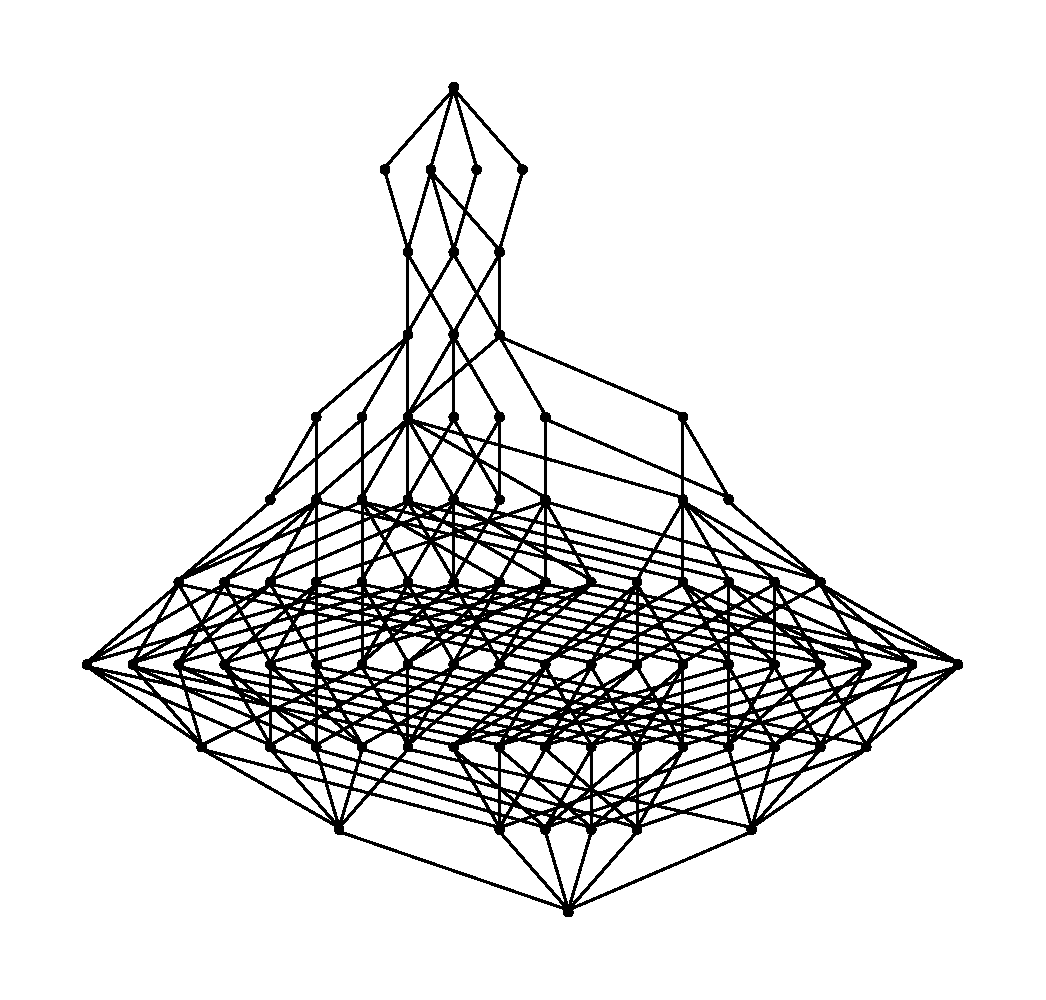
\includegraphics[width=\textwidth]{pics/ch-lattice/gossip3.pdf}
  \texttt{gap> Splash(DotString(LatticeOfCongruences(GossipMonoid(3))));}
  \caption[Congruence lattice of the Gossip monoid $G_3$]
  {Congruence lattice of the Gossip monoid $G_3$ \cite[\S2]{gossip}.  The
    semigroup contains $11$ elements, and the lattice contains $84$ congruences}
  \label{fig:g3-lattice}
\end{figure}

\begin{figure}[ht]
  \centering
  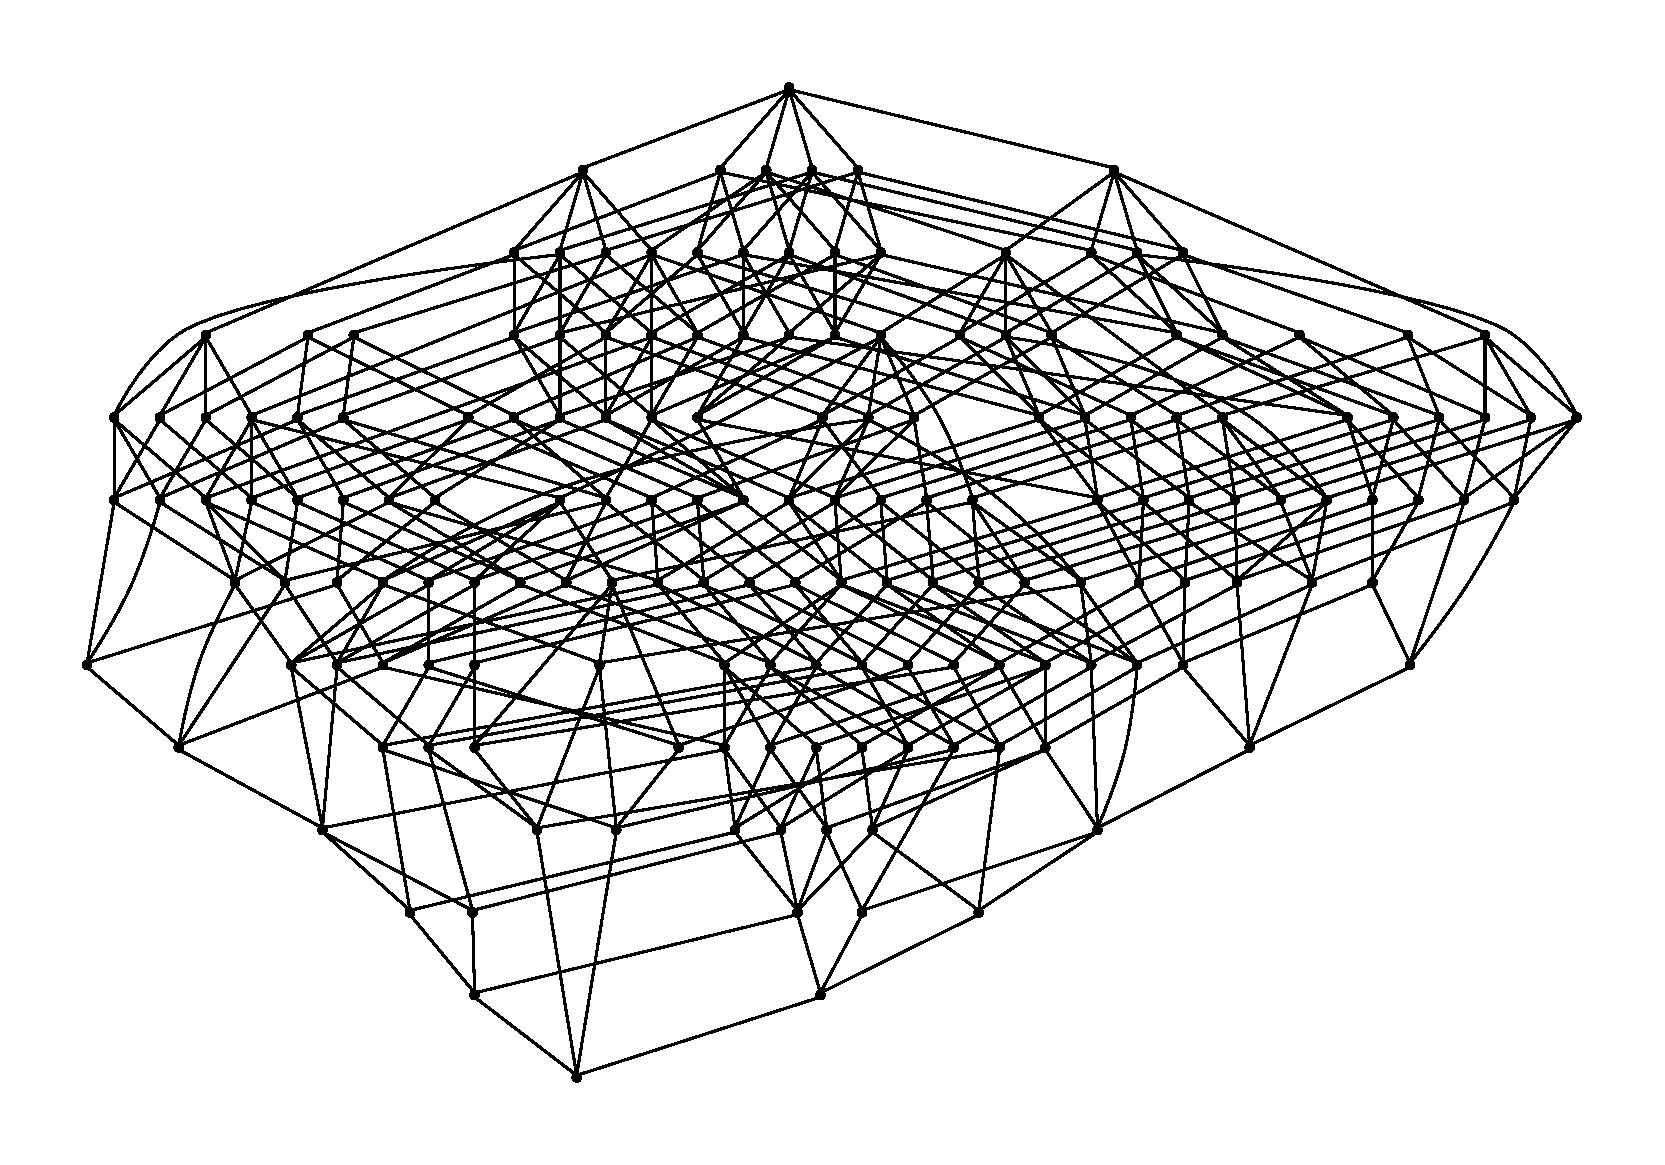
\includegraphics[width=\textwidth]{pics/ch-lattice/pbr1.pdf}
  \texttt{gap> Splash(DotString(LatticeOfCongruences(FullPBRMonoid(1))));}
  \caption[Congruence lattice of the full PBR monoid $\PBR_1$]
  {Congruence lattice of the full PBR monoid $\PBR_1$
    \cite[\S2.1]{diagram_semigroups}.  The semigroup contains $16$ elements, and
    the lattice contains $167$ congruences}
  \label{fig:pbr1-lattice}
\end{figure}

\begin{figure}[ht]
  \centering
  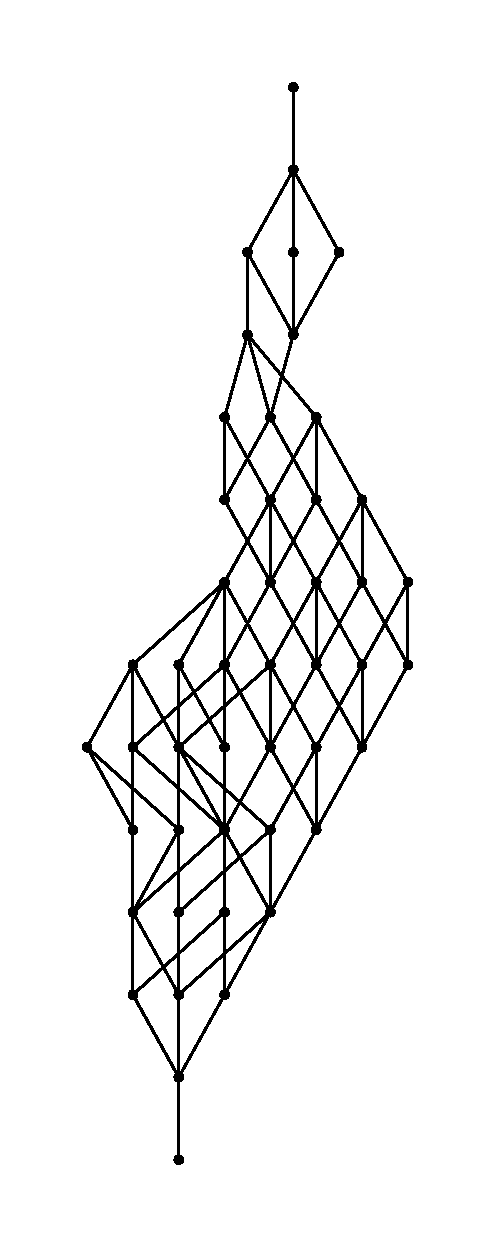
\includegraphics[height=0.8\textheight]{pics/ch-lattice/c2-wr-t3.pdf}
  \doublespacing
  \vspace{-1.5cm}
  \begin{align*}
    &\texttt{gap> C2 := Group((1, 2));;} \\
    &\texttt{gap> T3 := FullTransformationMonoid(3);;} \\
    &\texttt{gap> W := WreathProduct(C2, T3);;} \\
    &\texttt{gap> Splash(DotString(LatticeOfCongruences(W)));}
  \end{align*}
  \vspace{-1.0cm}
  \caption[Congruence lattice of the Wreath product $C_2 \wr \T_3$]
  {Congruence lattice of the Wreath product $C_2 \wr \T_3$
    \cite[\S10.1]{wreath}.  The semigroup contains $216$ elements, and the
    lattice contains $47$ congruences}
  \label{fig:c2-wr-t3-lattice}
\end{figure}

There are two main factors which determine how long
\texttt{LatticeOfCongruences} takes to compute the lattice: the size of the
semigroup $S$, and the number of congruences in the lattice $\Gamma$ itself.
Informal analysis shows that these two values do not necessarily go hand in
hand.  For instance, the monoids considered later in Section
\ref{sec:other-monoids-results} show a variety of numbers of congruences which
do not always correlate with the sizes of the semigroups.  Even Figures
\ref{fig:pbr1-lattice} and \ref{fig:c2-wr-t3-lattice} demonstrate between them
that an increase in semigroup size need not indicate an increase in number of
congruences.

In one test on an Intel Core i7-4770S CPU running at $3.10$GHz with 16GB of
memory, calculating the lattice of congruences of the wreath product
$C_2 \wr \T_3$ (Figure \ref{fig:c2-wr-t3-lattice}) took $3140$ ms, of which
almost all the time ($3019$ ms) was consumed by \textsc{PrincCongPoset}.  This
is because the semigroup is relatively large ($216$ elements), and therefore
iterating through all relevant pairs in $S \times S$ takes a long time; whereas
the number of congruences is relatively small (only $47$) meaning that the
taking of joins does not take long.  A contrasting example is the full PBR
monoid $\PBR_1$ (Figure \ref{fig:pbr1-lattice}): this took $5445$ ms in total,
of which almost all ($5422$ ms) was spent in \textsc{JoinClosure}.  This is
because the semigroup is relatively small (only $16$ elements), so iterating
through $S \times S$ is quick; but it has many congruences ($167$) meaning that
it takes a long time to compute all the joins.

Since it is unknown in advance how many congruences a semigroup has, it is
difficult to predict the feasibility of computing the lattice of a given
semigroup, even if its size is known.  Certainly all $853,303$ semigroups of
size up to $7$ have had their congruence lattices computed with the aid of the
\smallsemi{} library \cite{smallsemi}, and tests on randomly generated
transformation semigroups can usually calculate the lattice of a semigroup of
size up to 400 in less than a minute (on the previously mentioned computer).
However, we can choose very small examples in which \textsc{JoinClosure} runs
for an unreasonable amount of time.  Take, for example, the zero semigroup
$\Z_{10}$, with only $10$ elements.  Calculating all its congruences using the
method above does not complete within an hour, though computing the principal
congruences takes only $16$ milliseconds.  This is because $\Z_{10}$ has a large
number of congruences, given by the Bell number $B_{10} = 115975$, as will be
shown in Theorem \ref{thm:congruence-full}.  An alternative method would work
better here, since that theorem shows us that any equivalence on $\Z_{10}$ is a
congruence.

In both parts of the algorithm, most of the work consists of comparing
congruences to each other.  These comparisons can be done relatively quickly by
the efficient C++ code in \libsemigroups{} for generating pairs (see
Chapter \ref{chap:pairs}), but minimising the number of comparisons that need to
be made is nevertheless helpful for the algorithm's overall runtime.  Hence it
would be desirable, as future work, to improve the \textsc{PrincCongPoset}
algorithm somehow to avoid unnecessary comparisons, as well as to implement the
Froidure--Pin algorithm for \textsc{JoinClosure} in the \Semigroups{} package.

Since the algorithm described above was implemented in the \Semigroups{} package
\cite{semigroups}, it has been possible to compute the congruence lattice of
many semigroups.  Part \ref{part:results} of this thesis examines
the congruence lattices of a variety of semigroups, and attempts to explain
their structure.  Many of these lattices were originally computed using
\textsc{PrincCongPoset} and \textsc{JoinClosure}.  After examining these
lattices, it was possible in some cases to classify the congruences of entire
infinite families of semigroups, with proofs that were independent of any
computer code (see, for example, Theorems \ref{thm:mn-congs} and
\ref{thm:dkstar-congs}).  In others it was possible at least to produce
conjectures about families of semigroups, and to prove them for small cases (see
Conjectures \ref{conj:not-cong-full} and \ref{conj:cong-nearfull-7}).


\part{Theoretical results}
\label{part:results}
\chapter{Congruences of the Motzkin monoid}
\label{chap:motzkin}

In Chapter \ref{chap:lattice} we explained a relatively quick way of computing
all of a semigroup's congruences, along with information about how they fit into
their lattice structure.  This was implemented in the Semigroups package
\cite{semigroups}, greatly increasing the size and complexity of semigroups
whose congruence lattices can be found using a computer.

One of the first semigroups towards which this new methodology was directed was
the bipartition monoid $\Prt_n$, whose congruence lattice was not previously
known.  Computing this lattice for the first few values of $n$ showed a lattice
with a relatively simple structure, which did not appear to increase much in
complexity as $n$ grew higher than $3$.  The congruence lattices of various
submonoids of $\Prt_n$ were also computed, and appeared to have a similar
structure.  With the rapidly increasing size of $\Prt_n$ (see Table
\ref{tab:pn-size}) it proved impractical to na\"ively calculate the congruence
lattices beyond $n=4$, but careful study of the lattices for small values of
$n$, along with those lattices computed for various submonoids of $\Prt_n$,
yielded a general classification of the congruence lattice of $\Prt_n$ for
arbitrary $n$, along with a classification of the congruence lattices of various
important submonoids.  This classification is explained and proven in
\cite{ourpaper}, the paper upon which this chapter is based.

In this chapter, we will examine the structure of these congruence lattices,
focusing in particular on the Motzkin monoid $\Mot_n$, which was the present
author's particular focus when contributing to \cite{ourpaper}.  Much of this
content is contained in some form in that paper, and is included in this thesis
by the kind permission of my co-authors.  We will start with the definition of
the Motzkin monoid, then describe some preliminary theory, then describe the
Motzkin monoid's lattice of congruences (Theorem \ref{thm:mn-congs}), and
finally give a brief description of how these ideas can be extended to $\Prt_n$
and its other submonoids.

\section{The Motzkin monoid $\Mot_n$}
\label{sec:motzkin-monoid}
In order to define the Motzkin monoid, we must first define a \textit{planar}
bipartition.

\begin{definition}
  \label{def:planar}
  \index{planar bipartition}
  A bipartition is called \textbf{planar} if it can be represented in diagram
  form with all edges contained inside the rectangle formed by the vertices,
  without any edges crossing.
\end{definition}

\begin{example}
  Let $\alpha = \bipart{c|c|c|c}{2-4}{1,2 &3 &4 &5}{2,5 &1 &\mc2{c}{3,4}}$ and
  $\beta = \bipart{c|c|c|c}{3-4}{2 &5 &1,3 &4}{1 &3,4 &2 &5}$.  As can be seen
  in Figure \ref{fig:planar}, $\alpha$ is planar.  However, $\beta$ cannot be
  drawn inside the rectangle without the upper block $\{1,3\}$ crossing lines
  with the transversal $\{2, 1'\}$---hence, $\beta$ is not planar.
\end{example}

\begin{figure}[h]
  \centering
  $$\alpha = \bipartdiag{\tc12\tv22\bC25 \bc34} \qquad
  \beta = \bipartdiag{\tc13 \tv21 \tv54\bc34}$$
  \caption{A planar and a non-planar bipartition}
  \label{fig:planar}
\end{figure}

We can now define the Motzkin monoid.

\begin{definition}
  \label{def:motzkin}
  \index{Motzkin monoid}
  \nomenclature[Mn]{$\Mot_n$}{Motzkin monoid}
  The \textbf{Motzkin monoid} $\Mot_n$ is the submonoid of $\Prt_n$ consisting
  of all planar bipartitions of degree $n$ in which every block has size $1$ or
  $2$.
\end{definition}

To see that this is indeed a monoid, we should observe that it is closed.  It is
easy to see that the product of two planar bipartitions is also planar, since a
double diagram as in Figure \ref{fig:bipartition-example} would contain no
crossing lines, and therefore would resolve to a product with no crossing lines.
It is also easy to see that if two bipartitions have no block larger than $2$,
their product also has no block larger than $2$: any transversal can only
contain one point in $\bn$ and one point in $\bn'$, so any transversal in the
product can only contain two points.  The upper and lower blocks of the product
are inherited from the original bipartitions, so they will not break the
condition either.

The Motzkin monoid $\Mot_n$ grows much slower than its parent $\Prt_n$, having
only $\sum_{k=0}^n \binom{2n}{2k}C_k$ elements
\citeoeis{A026945}, where $C_k$ is the $k$th
Catalan number.  Its size in comparison with $\Prt_n$ is shown in Table
\ref{tab:mn-size}.

\begin{table}[h]
  \centering
  \renewcommand\arraystretch{1.0}
  \begin{tabular}{| r | r | r |}
    \hline
    $n$ & $|\Mot_n|$ & $|\Prt_n|$ \\
    \hline
     1 &           2 &                  2 \\
     2 &           9 &                 15 \\
     3 &          51 &                203 \\
     4 &         323 &              4 140 \\
     5 &       2 188 &            115 975 \\
     6 &      15 511 &          4 213 597 \\
     7 &     113 634 &        190 899 322 \\
     8 &     853 467 &     10 480 142 147 \\
     9 &   6 536 382 &    682 076 806 159 \\
    10 &  50 852 019 & 51 724 158 235 372 \\
    \hline
  \end{tabular}
  \renewcommand\arraystretch{0.7}
  \caption{Sizes of $\Mot_n$ and $\Prt_n$ for small values of $n$}
  \label{tab:mn-size}
\end{table}

The Motzkin monoid $\Mot_n$ shares a number of features with $\Prt_n$---indeed,
we will see later that its congruence lattice is very similar.  Like $\Prt_n$,
$\Mot_n$ is regular with a possible inverse given by the $^\star$
function. Another important similarity is in its Green's relations: consider the
following proposition, akin to Proposition \ref{prop:bipartition-greens}.

\begin{proposition}
  \label{prop:mn-greens}
  \nomenclature[Ik]{$I_k$}{Ideal of the Motzkin monoid $\Mot_n$}
  Let $\alpha$ and $\beta$ be bipartitions in $\Mot_n$.  The following hold:
  \begin{enumerate}[\rm(i)]
  \item $\alpha \RR \beta$ if and only if $\dom \alpha = \dom \beta$ and
    $\ker \alpha = \ker \beta$;
  \item $\alpha \LL \beta$ if and only if $\codom \alpha = \codom \beta$ and
    $\coker \alpha = \coker \beta$;
  \item $\alpha \JJ \beta$ if and only if $\rank \alpha = \rank \beta$;
  \item $J_\alpha \leq J_\beta$ if and only if $\rank \alpha \leq \rank \beta$;
  \item the ideals of $\Mot_n$ are precisely the sets
    $I_k=\{\alpha \in \Mot_n : \rank \alpha \leq k\}$ for
    $k \in \{0, \ldots, n\}$.
  \end{enumerate}
  \begin{proof}
    For (i) to (iii), see \cite[Theorem 2.4]{deg_motzkin}.  For (iv) and (v),
    see \cite[Proposition 2.6]{deg_motzkin}.
    % TODO: actually give the proof
  \end{proof}
\end{proposition}

This description of the Motzkin monoid's Green's relations, and its containment
of $\JJ$-classes and ideals, will help us greatly later on.  However, one
consequence of (i) and (ii) gives $\Mot_n$ a feature which $\Prt_n$ does not
share, namely the following corollary.

\begin{corollary}
  \label{cor:mn-h-trivial}
  The Motzkin monoid $\Mot_n$ is $\HH$-trivial.
  \begin{proof}
    Let $\alpha, \beta \in \Mot_n$ such that $\alpha \HH \beta$.  This tells us
    that $\alpha \LL \beta$ and $\alpha \RR \beta$, so by Proposition
    \ref{prop:mn-greens} parts (i) and (ii), we know that $\alpha$ and $\beta$
    share the same domain, kernel, codomain and cokernel.  The upper blocks and
    lower blocks of $\alpha$ and $\beta$ must certainly be the same, since they
    are just the blocks of the kernel and cokernel that do not lie in the domain
    or codomain.  The only choice is in the transversals: which blocks in the
    domain connect to which blocks in the codomain.  In $\Prt_n$ there are
    $(\rank \alpha)!$ ways of choosing this match-up; but in $\Mot_n$ there is
    only one way possible, since we cannot allow any lines in the diagram to
    cross.  Hence $\alpha = \beta$.
  \end{proof}
\end{corollary}

Finally, we will state one other feature of $\Mot_n$ which distinguishes it from
$\Prt_n$---an interesting property of its minimal ideal $I_0$.

\begin{lemma}
  \label{lem:i0-rect-band}
  Let $\alpha$ and $\beta$ be bipartitions in $I_0$, the minimal ideal of
  $\Mot_n$.  Then $\alpha \beta \alpha = \alpha$.
  % The product $\alpha\beta$ has the following proprties: $\ker\alpha\beta = \ker\alpha$,
  % $\coker\alpha\beta = \coker\beta$, and
  % $\dom\alpha\beta = \codom\alpha\beta = \varnothing$.
  \begin{proof}
    Since $\alpha$ has no transversals, $\alpha\beta\alpha$ also has no
    transversals.  The upper blocks of a product are equal to its first
    component, the lower blocks to its last component---so $\alpha\beta\alpha$
    has the upper and lower blocks of $\alpha$.  Hence it equals $\alpha$.
  \end{proof}
\end{lemma}

The lemma above establishes that $I_0$ is a \textit{rectangular band}, an
interesting class of regular semigroup---see \cite[\S4.4]{howie} for a
discussion of these. \index{rectangular band}

\section{Lifted congruences}
\label{sec:motzkin-prelim}
We will now define some concepts which allow us to find certain
congruences in any semigroup: \textit{retractable ideals} (Definition
\ref{def:retractable-ideal}) and \textit{liftable congruences} (Definition
\ref{def:liftable-congruence}).  It will turn out that all non-Rees congruences
of $\Mot_n$ can be found using these two building blocks.

\begin{definition}
  \label{def:retractable-ideal}
  \index{retractable ideal} \index{retraction}
  Let $S$ be a finite semigroup, with minimal ideal $M$.  An ideal $I$ of $S$ is
  called \textbf{retractable} if there exists some homomorphism $\phi: I \to M$
  such that $(m)\phi = m$ for all $m \in M$; we call $\phi$ a
  \textbf{retraction}.
\end{definition}

\begin{definition}
  \label{def:liftable-congruence}
  \index{liftable congruence}
  \nomenclature{$\sigma$}{Liftable congruence}
  Let $S$ be a finite semigroup, with minimal ideal $M$.  A congruence $\sigma$
  on $M$ is \textbf{liftable congruence} of $S$ if any, and therefore all, of
  the following equivalent conditions are satisfied:
  \begin{enumerate}[\rm(i)]
  \item $\sigma \cup \Delta_S$ is a congruence on $S$;
  \item there exists some congruence $\bar\sigma$ on $S$ such that
    $\sigma= \bar\sigma \cap (M \times M)$;
  \item $(ax,bx),(xa,xb) \in \sigma$ for all pairs $(a,b) \in \sigma$ and
    elements $x \in S$.
  \end{enumerate}
\end{definition}

In order to use these building blocks to produce new congruences, we first need
to establish some results about them.  Note that, since $\Mot_n$ is finite, it
must have a minimal ideal.  More specifically, the minimal ideal of $\Mot_n$ is
given by $I_0 = \{\alpha \in \Mot_n : \rank \alpha = 0\}$ (see Proposition
\ref{prop:mn-greens}).  The following lemma will be used at various times
throughout this chapter.

\begin{lemma}
  \label{lem:retract-aux}
  Let $S$ be a finite semigroup, with regular minimal ideal $M$, and let $I$ be
  an ideal of $S$.  If $I$ is retractable and $\phi: I \rightarrow M$ is a
  retraction from $I$ to $M$, then $(sxt)\phi=s \cdot (x)\phi \cdot t$ for all
  elements $x\in I$ and $s,t\in S^1$.
  \begin{proof}
    Firstly, let us consider left multiplication.  Since $M$ is regular, any
    element $m \in M$ has an inverse $m' \in M$, a left identity given by $mm'$,
    and a right identity given by $m'm$.  Let $e$ be a right
    identity for $(x)\phi$, so that
    $(x)\phi \cdot e = (x)\phi$.
    Since $\phi$ is a retraction and $e, xe \in M$, we have
    $$(x)\phi=(x)\phi \cdot e = (x)\phi \cdot (e)\phi = (xe)\phi = xe,$$
    so $(x)\phi = xe$.  Now let $f$ be a left identity for $(sx)\phi$; we also
    have
    \begin{align*}
      (sx)\phi \cdot e & = f \cdot (sx)\phi \cdot e \\
      & = (f)\phi \cdot (sx)\phi \cdot e \\
      & = (fsx)\phi \cdot e \\
      & = (fs)\phi \cdot (x)\phi \cdot e \\
      & = (fs)\phi \cdot (x)\phi \\
      & = (fsx)\phi \\
      & = (f)\phi \cdot (sx)\phi \\
      & = f \cdot (sx)\phi \\
      & = (sx)\phi,
    \end{align*}
    which shows that $e$ is a right identity for $(sx)\phi$ as well as for
    $(x)\phi$.  Hence we have
    $s \cdot (x)\phi = s \cdot xe = (sxe)\phi = (sx)\phi \cdot (e)\phi =
    (sx)\phi \cdot e = (sx)\phi$, so $\phi$ respects left multiplication; a
    symmetric argument gives $(xt)\phi = (x)\phi \cdot t$, so $\phi$ respects
    right multiplication too.  Finally we can combine these to give
    $(sxt)\phi = (sx)\phi \cdot t = s \cdot (x)\phi \cdot t$, as required.
  \end{proof}
\end{lemma}

This lemma gives rise to an important corollary which we can use later when we
combine retractable ideals with liftable congruences.  Note first that, since
$\Mot_n$ is a regular semigroup, its minimal ideal is also regular.

\begin{corollary}
  \label{cor:retract-unique}
  Let $S$ be a finite semigroup, with regular minimal ideal $M$.  If $I$ is a
  retractable ideal of $S$, then the retraction $\phi:I \to M$ is unique.
  \begin{proof}
    Let $\phi$ and $\psi$ be retractions from $I$ to $M$.  Let $x \in I$,
    and let $e_l$ and $e_r$ be left and right identities for $(x)\phi$.  By
    Lemma \ref{lem:retract-aux}, we have
    $$(x)\phi
    = e_l \cdot (x)\phi
    = (e_lx)\phi
    = e_lx
    = (e_lx)\psi
    = e_l \cdot (x)\psi,$$
    so $(x)\phi = e_l \cdot (x)\psi$, and a symmetric argument gives us
    $(x)\psi = (x)\phi \cdot e_r$.  But then
    $$(x)\phi
    = e_l \cdot (x)\psi
    = e_l \cdot (x)\phi \cdot e_r
    = (x)\phi \cdot e_r
    = (x)\psi,$$
    so $\phi = \psi$.
  \end{proof}
\end{corollary}

The effect of Corollary \ref{cor:retract-unique} is that, for a semigroup with a
regular minimal ideal, we can talk about \textit{the} retraction of a
retractable ideal without any loss of generality.  This result is the last thing
we need to use our two building blocks to produce a new congruence: a
\textit{lifted congruence}.

\begin{definition}
  \label{def:lifted-congruence}
  \index{lifted congruence}
  \nomenclature{$\zeta_{I,\sigma}$}{Lifted congruence}
  Let $S$ be a semigroup with a minimal ideal $M$, let $I$ be a retractable
  ideal of $S$, and let $\sigma$ be a liftable congruence of $S$.  We associate
  to the pair $(I,\sigma)$ the relation
  $$\zeta_{I,\sigma}
  = \{(x,y) \in I \times I : (x\phi,y\phi) \in \sigma\} \cup \Delta_S,$$
  where $\phi$ is the unique retraction $I \to M$.
  We call $\zeta_{I,\sigma}$ the \textbf{lifted congruence} of $(I,\sigma)$.
\end{definition}

In order to justify the name \textit{lifted congruence}, we require the
following proposition.

\begin{theorem}
  \label{thm:lifted-congruence}
  The relation $\zeta_{I,\sigma}$ in Definition \ref{def:lifted-congruence} is a
  congruence on $S$.
  \begin{proof}
    For conciseness, let us refer to $\zeta_{I,\sigma}$ as $\zeta$.  Let $(x,y)$
    be a pair in $\zeta$ and let $s \in S$.  To show $\zeta$ is a congruence, we
    must show that $(sx,sy)$ and $(xs,ys)$ both lie in $\zeta$.  If
    $(x,y) \in \Delta_S$, this is certainly true.  Otherwise, we have
    $x, y \in I$ and $(x\phi, y\phi) \in \sigma$.  Since $I$ is an ideal, we
    certainly have $xs,ys\in I$.  Now by Definition
    \ref{def:liftable-congruence} part (iii), and by Lemma
    \ref{lem:retract-aux}, we have
    $(sx)\phi = s \cdot (x)\phi \mathrel\sigma s \cdot (y)\phi = (sy)\phi$, so
    that $(sx, sy) \in \zeta$.  A symmetric argument gives us
    $(xs,ys) \in \zeta$.
  \end{proof}
\end{theorem}

This construction now gives us a usable source of congruences.  All that is
required is to find some liftable congruences and retractable ideals of a
semigroup, and a number of new congruences can be described.  It turns out that
this is an excellent source of congruences for $\Mot_n$, yielding every non-Rees
congruence on the semigroup, as we will see later.

\section{Congruence lattice of $\Mot_n$}
\label{sec:motzkin-congs}

% Rees congruences

We can now apply the general theory of Section \ref{sec:motzkin-prelim} to the
Motzkin monoid, in order to find its congruences.  First, let us mention the
easiest congruences to describe---its Rees congruences (Definition
\ref{def:rees-congruence}).

\begin{proposition}
  \label{prop:motzkin-rees}
  \nomenclature[Rk]{$R_k$}{Rees congruence of the Motzkin monoid $\Mot_n$}
  The Rees congruences of $\Mot_n$ are the relations
  $$R_k = \{(x,y) \in \Mot_n \times \Mot_n : \rank x, \rank y \leq k\} \cup
  \Delta_{\Mot_n},$$
  for $k \in \{0, \ldots, n\}$.
  \begin{proof}
    This follows immediately from the description of the ideals of $\Mot_n$ in
    Proposition \ref{prop:mn-greens} part (v).
  \end{proof}
\end{proposition}

We will refer to these congruences by the name $R_k$ for the rest of this
chapter.  We will soon see that $R_0$ and $R_1$ are in fact lifted congruences,
but the higher Rees congruences may not be.  Next, we will describe some other
lifted congruences, by identifying some liftable congruences and retractions in
$\Mot_n$ to use as building blocks.

% L,R,H,Delta,Univ are liftable congs: lambda, rho, mu, eta, R
First, recall that $I_0 = \{\alpha \in \Mot_n : \rank \alpha = 0\}$ is the
minimal ideal of $\Mot_n$.  Let us denote by $\LL_0$ and $\RR_0$ the $\LL$ and
$\RR$ relations of $\Mot_n$ restricted to $I_0$, and let $\Delta_0$ and
$\nabla_0$ be abbreviations for $\Delta_{I_0}$ and $\nabla_{I_0}$ respectively.
\nomenclature{$\Delta_0$}{Trivial congruence on the ideal $I_0$}
\nomenclature{$\nabla_0$}{Universal congruence on the ideal $I_0$}
\nomenclature[L0]{$\LL_0$}{Green's $\LL$ relation retricted to the ideal $I_0$}
\nomenclature[R0]{$\RR_0$}{Green's $\RR$ relation retricted to the ideal $I_0$}

\begin{proposition}
  The relations $\Delta_0$, $\LL_0$, $\RR_0$ and $\nabla_0$ are all
  liftable congruences of $\Mot_n$.
  \begin{proof}
    Since $I_0$ is a semigroup, $\Delta_0$ and $\nabla_0$ are certainly
    congruences of $I_0$; and both satisfy Definition
    \ref{def:liftable-congruence} (i), since their unions with $\Delta_{\Mot_n}$
    are the congruences $\Delta_{\Mot_n}$ and $R_0$ respectively.

    To see that $\LL_0$ is a liftable congruence, consider Definition
    \ref{def:liftable-congruence} (iii); let $(a,b) \in \LL_0$ and
    $x \in \Mot_n$.  Since $I_0$ is the minimal ideal, we certainly have
    $xa,xb,ax,bx \in I_0$.  And since $\LL$ is a right congruence on $\Mot_n$
    (see Proposition \ref{prop:greens-as-congs}) we have $(ax,bx) \in \LL$ and
    therefore $(ax,bx) \in \LL_0$.  By Lemma \ref{lem:i0-rect-band} we also have
    $a(xa) = a$, so $xa \LL a$ and similarly $xb \LL b$.  This means that
    $xa \LL a \LL b \LL xb$, so $(xa, xb) \in \LL_0$.  Hence $\LL_0$ is a
    liftable congruence of $\Mot_n$, and by a similar argument, so is $\RR_0$.
  \end{proof}
\end{proposition}

% ^ notation
Now that we have some liftable congruences, we also want some retractable ideals
in order to form lifted congruences.  The following construction establishes one
such ideal.

\begin{definition}
  \label{def:mn-hat}
  \nomenclature[^]{$\widehat{\phantom\alpha}$}{Bipartition of rank $0$ with this
    kernel and cokernel}
  If $\alpha$ is a bipartition, then $\widehat\alpha$ is the unique bipartition
  of rank $0$ with the same kernel and cokernel as $\alpha$.
\end{definition}

The element $\widehat\alpha$ can be computed easily from $\alpha$: each
transversal is split into an upper block (the points in $\bn$) and a lower block
(the points in $\bn'$) and nothing else is changed.  If we have a diagram for
$\alpha$, drawn in the standard way described after Example
\ref{ex:bipartition}, then we simply remove any lines crossing the diagram.  If
we are using two-row notation, we can simply draw a horizontal line between the
two rows.  See Figure \ref{fig:hat} for an example.  Note that $\widehat\alpha =
\alpha$ for all $\alpha \in I_0$.

\begin{figure}[h]
  \centering
  $$\alpha = \big\{
    \{1,3,4,1'\}, \{2,3',4'\}, \{5\}, \{2'\}, \{5'\}
  \big\}$$
  $$\widehat\alpha = \big\{
    \{1,3,4\}, \{1'\}, \{2\}, \{3',4'\}, \{5\}, \{2'\}, \{5'\}
  \big\}$$
  $$\alpha = \bipartdiag{\tv11\tc13\tc34 \tv23\bc34} \quad
  \widehat\alpha = \bipartdiag{\tc13\tc34 \bc34}$$
  $$\alpha = \bipart{c|c|c|c}{3-4}{1,3,4 & 2 & \mc2c5}{1 & 3,4 & 2 & 5} \quad
  \widehat\alpha = \bipart{c|c|c|c}{1-4}{1,3,4 & 2 & \mc2c5}{1 & 3,4 & 2 & 5}$$
  \caption{Computing $\widehat\alpha$ from $\alpha$}
  \label{fig:hat}
\end{figure}

% Show ^:I1->I0 is a retraction
\begin{proposition}
  \label{prop:hat-retraction}
  The map $\phi: I_1 \to I_0$ defined by $\alpha \mapsto \widehat\alpha$ is a
  retraction.  Hence, $I_1$ is a retractable ideal.
  \begin{proof}
    First, we will show that $\phi$ is a homomorphism.  Let
    $\alpha,\beta \in I_1$---we will try to prove that
    $\widehat{\alpha\beta} = \widehat\alpha \widehat\beta$.  If both $\alpha$
    and $\beta$ have rank $0$ then
    $\widehat{\alpha\beta} = \alpha\beta = \widehat\alpha \widehat\beta$.  On
    the other hand, if at least one of $\alpha$ and $\beta$ has rank $1$ (without
    loss of generality, $\alpha$) then we may write
    $\alpha = \bipart{c|c|c|c}{2-4}{A_0&A_1&\ldots&A_r}{B_0&B_1&\ldots&B_s}$ and
    $\beta = \bipart{c|c|c|c}{2-4}{C_0&C_1&\ldots&C_t}{D_0&D_1&\ldots&D_u}$ or
    $\beta = \bipart{c|c|c|c}{1-4}{C_0&C_1&\ldots&C_t}{D_0&D_1&\ldots&D_u}$.
    This gives us
    $\alpha\beta =
    \bipart{c|c|c|c}{2-4}{A_0&A_1&\ldots&A_r}{D_0&D_1&\ldots&D_u}$ or
    $\alpha\beta =
    \bipart{c|c|c|c}{1-4}{A_0&A_1&\ldots&A_r}{D_0&D_1&\ldots&D_u}$.  Applying
    $\phi$ gives us
    $\widehat\alpha =
    \bipart{c|c|c|c}{1-4}{A_0&A_1&\ldots&A_r}{B_0&B_1&\ldots&B_s}$,
    $\widehat\beta =
    \bipart{c|c|c|c}{1-4}{C_0&C_1&\ldots&C_t}{D_0&D_1&\ldots&D_u}$, and finally
    $\widehat{\alpha\beta} =
    \bipart{c|c|c|c}{1-4}{A_0&A_1&\ldots&A_r}{D_0&D_1&\ldots&D_u} =
    \widehat\alpha \widehat\beta$, so $\phi$ is a homomorphism.  Since
    $\widehat\alpha = \alpha$ for $\alpha \in I_0$, we can see that $\phi$ is a
    retraction, as required.
  \end{proof}
\end{proposition}

This gives us a retractable ideal $I_1$, with a retraction
$\alpha \mapsto \widehat\alpha$.  It is also trivial to see that $I_0$ itself is
retractable, with retraction $\alpha \mapsto \alpha$, the identity map.  Since
the minimal ideal $\I_0$ is regular, Corollary \ref{cor:retract-unique} shows
that these retractions are unique.

% Describe the congruences:
% mu0, lam0, rho0, R0,
% mu1, lam1, rho1, R1,
% R2 ... Rn
We now have four liftable congruences $\{\Delta_0, \LL_0, \RR_0, \nabla_0\}$ and
two retractable ideals $\{I_0, I_1\}$, giving rise to $4 \times 2 = 8$ lifted
congruences by Definition \ref{def:lifted-congruence} and Theorem
\ref{thm:lifted-congruence}.  The congruences lifted from $\nabla_0$ are
observed to be equal to the Rees congruences $R_0$ and $R_1$, while those lifted
from $\Delta_0$, $\LL_0$ and $\RR_0$ are named with appropriate Greek symbols,
as follows.
\begin{align*}
  \delta_0 &= \zeta_{I_0,\Delta_0}
  = \{(\alpha,\beta) \in I_0 \times I_0 :
    (\alpha, \beta) \in \Delta_0\} \cup \Delta_{\Mot_n} \\
  \delta_1 &= \zeta_{I_1,\Delta_0}
  = \{(\alpha,\beta) \in I_1 \times I_1 :
    (\widehat\alpha, \widehat\beta) \in \Delta_0\} \cup \Delta_{\Mot_n} \\
  \lambda_0 &=\zeta_{I_0,\LL_0}
  = \{(\alpha,\beta) \in I_0 \times I_0 :
    (\alpha, \beta) \in \LL_0\} \cup \Delta_{\Mot_n} \\
  \lambda_1 &= \zeta_{I_1,\LL_0}
  = \{(\alpha,\beta) \in I_1 \times I_1 :
    (\widehat\alpha, \widehat\beta) \in \LL_0\} \cup \Delta_{\Mot_n} \\
  \rho_0 &= \zeta_{I_0,\RR_0}
  = \{(\alpha,\beta) \in I_0 \times I_0 :
    (\alpha, \beta) \in \RR_0\} \cup \Delta_{\Mot_n} \\
  \rho_1 &= \zeta_{I_1,\RR_0}
  = \{(\alpha,\beta) \in I_1 \times I_1 :
    (\widehat\alpha, \widehat\beta) \in \RR_0\} \cup \Delta_{\Mot_n} \\
  R_0 &= \zeta_{I_0,\nabla_0}
  = \{(\alpha,\beta) \in I_0 \times I_0 :
    (\alpha, \beta) \in \nabla_0\} \cup \Delta_{\Mot_n} \\
  R_1 &= \zeta_{I_1,\nabla_0}
  = \{(\alpha,\beta) \in I_1 \times I_1 :
    (\widehat\alpha, \widehat\beta) \in \nabla_0\} \cup \Delta_{\Mot_n}
\end{align*}

This naming convention is summarised in Table \ref{tab:mn-lifted-congruences}.

\begin{table}[h]
  \centering
  \renewcommand\arraystretch{1.0}
  \begin{tabular}[h]{| c | c | c |}
    \cline{2-3}
    \mc1{c|}{} & $I_0$ & $I_1$ \\ \hline
    $\Delta_0$ & $\delta_0$ & $\delta_1$ \\ \hline
    $\LL_0$ & $\lambda_0$ & $\lambda_1$ \\ \hline
    $\RR_0$ & $\rho_0$ & $\rho_1$ \\ \hline
    $\nabla_0$ & $R_0$ & $R_1$ \\ \hline
  \end{tabular}
  \caption{Lifted congruences of $\Mot_n$}
  \label{tab:mn-lifted-congruences}
\end{table}

Interpreting these statements along with the use of Proposition
\ref{prop:mn-greens} gives the following characterisation of the lifted
congruences in terms of a bipartition's rank, kernel and cokernel.

\begin{proposition}
  \label{prop:mn-cong-char}
  The lifted congruences of $\Mot_n$ can be characterised in the following way,
  where $(\alpha, \beta) \in \Mot_n \times \Mot_n$:
  \begin{align*}
    \delta_0 &= \Delta_{\Mot_n} \\
    \delta_1 &= \{(\alpha,\beta) :
                  \rank\alpha,\rank\beta \leq 1,
                  \ker\alpha = \ker\beta,
                  \coker\alpha = \coker\beta\} \cup \Delta_{\Mot_n} \\
    \lambda_0 &= \{(\alpha,\beta) :
                   \rank\alpha,\rank\beta = 0,
                   \coker\alpha = \coker\beta\} \cup \Delta_{\Mot_n} \\
    \lambda_1 &= \{(\alpha,\beta) :
                   \rank\alpha,\rank\beta \leq 1,
                   \coker\alpha = \coker\beta\} \cup \Delta_{\Mot_n} \\
    \rho_0 &= \{(\alpha,\beta) :
                \rank\alpha,\rank\beta = 0,
                \ker\alpha = \ker\beta\} \cup \Delta_{\Mot_n} \\
    \rho_1 &= \{(\alpha,\beta) :
                \rank\alpha,\rank\beta \leq 1,
                \ker\alpha = \ker\beta\} \cup \Delta_{\Mot_n} \\
    R_0 &= \{(\alpha,\beta) :
             \rank\alpha,\rank\beta = 0\} \cup \Delta_{\Mot_n} \\
    R_1 &= \{(\alpha,\beta) :
             \rank\alpha,\rank\beta \leq 1\} \cup \Delta_{\Mot_n}
  \end{align*}
\end{proposition}
These characterisations will help us later when we consider generating pairs for
the congruences.

We are now ready to state the main theorem of this chapter, giving a full
description of the congruence lattice of $\Mot_n$.  Much of the work to prove
this has already been done, and the rest of this section will be devoted to
completing the proof.  Note that our main theorem requires $n \geq 2$; if
$n = 1$ then $\Mot_n$ has only $2$ elements, and its congruences are only
$\Delta_{\Mot_n}$ and $\nabla_{\Mot_n}$.

\begin{theorem}
  \label{thm:mn-congs}
  Let $\Mot_n$ be the Motzkin monoid, with $n \geq 2$.  The following hold:
  \begin{enumerate}[\rm(i)]
  \item The congruences of $\Mot_n$ are precisely
    $\{\delta_0, \delta_1, \lambda_0, \lambda_1, \rho_0, \rho_1, R_0, R_1,
    \ldots, R_n\}$;
  \item The congruence lattice of $\Mot_n$ is shown in Figure
    \ref{fig:mn-cong-lattice};
  \item Every congruence of $\Mot_n$ is principal;
  \item Each congruence $\sigma$ of $\Mot_n$ is generated by any single pair
    from $\sigma$ not contained in any congruence below $\sigma$ in the
    congruence lattice.
  \end{enumerate}
  \begin{proof}
    Let $\Gamma$ be the set of relations stated in (i).  That the relations in
    $\Gamma$ are congruences has already been established.  Table
    \ref{tab:mn-genpairs} summarises the conditions for a single pair in
    $\Mot_n \times \Mot_n$ to generate each congruence in $\Gamma$; it proves
    that every congruence in $\Gamma$ is principal, and since each pair in
    $\Mot_n \times \Mot_n$ satisfies one of the conditions, it proves that there
    are no other principal congruences.  Lemmas \ref{lem:mn-lattice-intra} and
    \ref{lem:mn-lattice-inter} show that the joins of these principal
    congruences are as shown in Figure \ref{fig:mn-cong-lattice}---proving
    (ii)---and therefore that $\Gamma$ is closed under taking joins, proving
    that $\Mot_n$ has no other congruences.  This completes the proof of (i) and
    (iii), and inspection of Table \ref{tab:mn-genpairs} establishes (iv).
  \end{proof}
\end{theorem}

% Show the lattice
\begin{figure}[h]
  \centering
  \begin{tikzpicture}
    [cong/.style={circle, minimum size=0.9cm, draw}]
    \node[cong] (Rn) at ( 0,13) {$R_n$};
    \node[cong] (R2) at ( 0,10) {$R_2$};
    \node[cong] (R1) at ( 0, 8) {$R_1$};
    \node[cong] (l1) at (-3, 6) {$\lambda_1$};
    \node[cong] (R0) at ( 0, 6) {$R_0$};
    \node[cong] (r1) at ( 3, 6) {$\rho_1$};
    \node[cong] (l0) at (-3, 4) {$\lambda_0$};
    \node[cong] (d1) at ( 0, 4) {$\delta_1$};
    \node[cong] (r0) at ( 3, 4) {$\rho_0$};
    \node[cong] (d0) at ( 0, 2) {$\delta_0$};
    \node at (1.17,13) {$=\nabla_{\Mot_n}$};
    \node at (1.17, 2) {$=\Delta_{\Mot_n}$};
    \draw (d0)--(l0) (d0)--(r0) (l0)--(R0) (r0)--(R0);
    \fill[white] (-1.5,5)circle(.15) (+1.5,5)circle(.15);
    \draw (d0)--(d1) (l0)--(l1) (r0)--(r1) (R0)--(R1);
    \draw (d1)--(l1) (d1)--(r1) (l1)--(R1) (r1)--(R1);
    \draw (R1)--(R2);
    \draw[dashed] (R2)--(Rn);
  \end{tikzpicture}
  \caption{Congruence lattice of $\Mot_n$ (Hasse diagram)}
  \label{fig:mn-cong-lattice}
\end{figure}

% Proof of exhaustion: table of generating pairs, with references to
% propositions
For the rest of this section, we will state the lemmas required to complete the
proof of Theorem \ref{thm:mn-congs}.  Firstly, we will focus on generating
pairs; we will consider a pair $(\alpha, \beta)$ and decide which principal
congruence it generates.  Our findings are summarised in Table
\ref{tab:mn-genpairs}.

\begin{table}[h]
  \renewcommand\arraystretch{1.0}
  \centering
  \begin{tabular}{| c | l | l |}
    \hline
    $(\alpha,\beta)^\sharp$ & $(\alpha,\beta) \in$ & Reference \\
    \hline
    $\delta_0$   & $\delta_0$
                 & Trivial                             \\
    $\delta_1$   & $\delta_1 \setminus \delta_0$
                 & Lemma \ref{lem:low-genpairs} (iii)  \\
    $\lambda_0$  & $\lambda_0 \setminus \delta_0$
                 & Lemma \ref{lem:low-genpairs} (i)    \\
    $\lambda_1$  & $\lambda_1 \setminus (\lambda_0 \cup \delta_1)$
                 & Lemma \ref{lem:high-genpairs} (i)   \\
    $\rho_0$     & $\rho_0 \setminus \delta_0$
                 & Lemma \ref{lem:low-genpairs} (ii)   \\
    $\rho_1$     & $\rho_1 \setminus (\rho_0 \cup \delta_1)$
                 & Lemma \ref{lem:high-genpairs} (ii)  \\
    $R_0$        & $R_0 \setminus (\lambda_0 \cup \rho_0)$
                 & Lemma \ref{lem:high-genpairs} (iii) \\
    $R_1$        & $R_1 \setminus (\lambda_1 \cup \rho_1 \cup R_0)$
                 & Lemma \ref{lem:high-genpairs} (iv)  \\
    $R_{k \geq 2}$ & $R_k \setminus R_{k-1}$
                 & Lemma \ref{lem:rees-genpairs}       \\
    \hline
  \end{tabular}
  \caption{Generating pairs for each congruence on $\Mot_n$}
  \label{tab:mn-genpairs}
\end{table}

\begin{lemma}
  \label{lem:low-genpairs}
  Let $\alpha,\beta \in \Mot_n$.  The following hold:
  \begin{enumerate}[\rm(i)]
  \item $\lambda_0 = (\alpha, \beta)^\sharp$ if and only if
    $(\alpha,\beta) \in \lambda_0 \setminus \Delta$;
  \item $\rho_0 = (\alpha, \beta)^\sharp$ if and only if
    $(\alpha,\beta) \in \rho_0 \setminus \Delta$;
  \item $\delta_1 = (\alpha, \beta)^\sharp$ if and only if
    $(\alpha,\beta) \in \delta_1 \setminus \Delta$.
  \end{enumerate}
  \begin{proof}
    In each statement, the ``only if'' part is obvious.  We will prove (i) and
    observe that (ii) follows from a symmetric argument.  Then we will prove
    (iii) separately. % TODO: make this precise, with "duality"?

    For (i), let $(\alpha, \beta) \in \lambda_0 \setminus \Delta$, and let
    $\sigma = (\alpha, \beta)^\sharp$.  Since $\lambda_0$ is a congruence, we
    clearly have $\sigma \subseteq \lambda_0$; hence we have only to prove that
    $\lambda_0 \subseteq \sigma$.  First we require a special construction: if
    $\gamma \in I_0$, let $\gamma'$ be the unique bipartition in $I_0$ with
    trivial kernel and $\coker\gamma' = \coker\gamma$.  We claim that
    $(\gamma, \gamma') \in \sigma$ for any such $\gamma$.  This claim is proven
    by descending induction on $r$, the number of kernel-classes of $\gamma$: if
    $r = n$ (trivial kernel) then $\gamma = \gamma'$ and we are done.  Otherwise
    we have $r \leq n-1$, and we write
    $\gamma = \bipart{c|c|c}{1-3}{A_1&\ldots&A_r}{B_1&\ldots&B_s}$.  Since
    $(\alpha,\beta) \in \lambda_0 \setminus \Delta$, Propisition
    \ref{prop:mn-cong-char} gives us $\rank\alpha = \rank\beta = 0$ and
    $\coker\alpha = \coker\beta$, but since $\alpha \neq \beta$ we must have
    $\ker\alpha \neq \ker\beta$.  Swapping $\alpha$ and $\beta$ if necessary,
    let us assume there exists some $(i,j) \in \ker\alpha \setminus \ker\beta$,
    and without loss of generality, assume $i < j$.  We will write
    $\bn \setminus \{i,j\}$ as $\{k_1, \ldots, k_{n-2}\}$.  Since $r \leq n-1$
    there exists some kernel block of $\gamma$ with 2 elements; let $m$
    be the lowest point in $\bn$ in a non-trivial kernel block, and without loss
    of generality, let us assume $m$ lies in $A_1$.  We can now define the
    bipartition $\tau = \bipart{c|c|c|c|c}{3-5}
    {m & p & A_2 & \ldots & A_r}
    {i & j & k_1 & \ldots & k_{n-2}}$, 
    where $A_1 = \{m, p\}$.
    We observe that $\tau \alpha \gamma = \gamma = \bipart{c|c|c|c|c}{1-5}
    {\mc2{c|}{m,p} & A_2 & \ldots & A_r}
    {B_1 & B_2 & B_3 & \ldots & B_s}$ and
    $\tau \beta \gamma = \bipart{c|c|c|c|c}{1-5}
    {m & p & A_2 & \ldots & A_r}
    {B_1 & B_2 & B_3 & \ldots & B_s}$.
    Since $\sigma$ is left- and right-compatible, we have
    $\gamma = \tau\alpha\gamma \mathrel\sigma \tau\beta\gamma$.  Hence $\gamma$
    is $\sigma$-related to $\tau\beta\gamma$, a bipartition with rank $0$, the
    same cokernel as $\gamma$, and $r+1$ kernel classes.  Applying the same
    process inductively, with $\tau\beta\gamma$ in place of $\gamma$, implies a
    chain of $\sigma$-relations which relate $\gamma$ to a bipartition with rank
    $0$, the same cokernel as $\gamma$, and $n$ kernel classes---that is,
    $\gamma'$.  This proves the claim that $(\gamma, \gamma') \in \sigma$.

    To return to the proof that $\lambda_0 \subseteq \sigma$, let
    $(\mu, \nu) \in \lambda_0$ be arbitrary.  If $\mu = \nu$ then certainly
    $(\mu, \nu) \in \sigma$, so let us assume $\mu \neq \nu$.  By Proposition
    \ref{prop:mn-cong-char} we must have $\rank\mu = \rank\nu = 0$ and
    $\coker\mu = \coker\nu$, so we have $\mu' = \nu'$.  Hence, by the above
    claim, we have $\mu \mathrel\sigma \mu' = \nu' \mathrel\sigma \nu$,
    so $(\mu, \nu) \in \sigma$, and (i) is complete.  Observe that (ii) follows
    by a similar argument.

    To prove (iii), let $(\alpha,\beta)\in\delta_1\setminus\Delta$ as stated,
    and let $\sigma = (\alpha,\beta)^\sharp$.  Clearly
    $\sigma \subseteq \delta_1$; it remains to prove that
    $\delta_1 \subseteq \sigma$.  Since
    $(\alpha,\beta) \in \delta_1 \setminus \Delta$, $\alpha$ and $\beta$ must
    each have rank $0$ or $1$, and have the same kernel and
    cokernel, but be distinct.  Since there is only one bipartition of rank $0$
    with a given kernel and cokernel, they cannot both have rank $0$.  Hence,
    swapping $\alpha$ and $\beta$ if necessary, we may assume that
    $\rank(\alpha)=1$, with transversal $\{i,j'\}$, and we can write
    $\alpha=\bipart{c|c|c|c}{2-4}
    {i & A_1 & \cdots & A_r}{j & B_1 & \cdots & B_s}$.
    Then $\beta$ has one of the following four forms, where without loss of
    generality, additional labelled elements are assumed to be from $A_1$:
    \begin{enumerate}[\rm(a)]
    \item $\beta = \bipart{c|c|c|c|c}{1-5}
      {i & A_1 & A_2 & \cdots & A_r}{j & B_1 & B_2 & \cdots & B_s}$,
      so that $\beta = \widehat\alpha$;
    \item $\beta = \bipart{c|c|c|c|c}{2-5}
      {k & i & A_2 & \cdots & A_r}{j & B_1 & B_2 & \cdots & B_s}$,
      replacing $i$ with $k$, a different point from $\bn$;
    \item $\beta = \bipart{c|c|c|c|c}{2-5}
      {i & A_1 & A_2 & \cdots & A_r}{l & j & B_2 & \cdots & B_s}$,
      replacing $j'$ with $l'$, a different point from $\bn'$;
    \item $\beta = \bipart{c|c|c|c|c}{2-5}
      {k & i & A_2 & \cdots & A_r}{l & j & B_2 & \cdots & B_s}$,
      with a completely different transversal from $\alpha$.
    \end{enumerate}
    Now, let us denote by $\tau_{ab}$ the bipartition
    $(a, b')^e \in \Mot_n$---this has just one non-trivial block, $\{a,b'\}$.
    We will use the bipartitions $\tau_{ii}$ and $\tau_{jj}$. In all four cases
    above, we have
    $\tau_{ii}\alpha\tau_{jj}= \tau_{ij}$ and
    $\tau_{ii}\beta\tau_{jj}= \tau_\varnothing$, the bipartition consisting
    entirely of singletons.  Since $\alpha \mathrel\sigma \beta$, we also have
    $\tau_{ii}\alpha\tau_{jj} \mathrel\sigma \tau_{ii}\beta\tau_{jj}$, so
    $\tau_{ij} \mathrel\sigma \tau_\varnothing$.
    Next, let $\gamma$ be an arbitrary bipartition in $\Mot_n$ with rank $1$.
    We can write
    $\gamma = \bipart{c|c|c|c}{2-4}
    {c & C_1 & \cdots & C_t}{d & D_1 & \cdots & D_u}$,
    where $\{c,d'\}$ is the one transversal.  Let us write
    $\bn \setminus \{i\} = \{i_1, \ldots, i_{n-1}\}$ and
    $\bn \setminus \{j\} = \{j_1, \ldots, j_{n-1}\}$.  Then we can define two
    new bipartitions:
    $\overline\gamma = \bipart{c|c|c|c}{2-4}
    {c & C_1 & \cdots & C_t}{i & i_1 & \cdots & i_{n-1}}$ and
    $\underline\gamma = \bipart{c|c|c|c}{2-4}
    {j & j_1 & \cdots & j_{n-1}}{d & D_1 & \cdots & D_u}$.
    We can see that $\gamma = \overline\gamma \tau_{ij} \underline\gamma$ and
    $\widehat\gamma = \overline\gamma \tau_\varnothing \underline\gamma$, so
    we have $\gamma \mathrel\sigma \widehat\gamma$ for any $\gamma$ of rank
    $1$.  The same statement is also true for $\gamma$ of rank $0$, since
    $\gamma = \widehat\gamma$.

    To prove that $\delta_1 \subseteq \sigma$, let $(\mu, \nu) \in \delta_1$ be
    arbitrary.  Each of $\mu$ and $\nu$ must have rank $0$ or $1$, and they must
    have the same kernel and cokernel.  Hence we have
    $\mu \mathrel\sigma \widehat\mu = \widehat\nu \mathrel\sigma \nu$, so
    $(\mu, \nu) \in \sigma$, completing the proof of (iii).
  \end{proof}
\end{lemma}

\begin{lemma}
  \label{lem:high-genpairs}
  Let $\alpha,\beta \in \Mot_n$.  The following hold:
  \begin{enumerate}[\rm(i)]
  \item $\lambda_1 = (\alpha, \beta)^\sharp$ if and only if
    $(\alpha,\beta) \in \lambda_1 \setminus (\lambda_0 \cup \delta_1)$;
  \item $\rho_1 = (\alpha, \beta)^\sharp$ if and only if
    $(\alpha,\beta) \in \rho_1 \setminus (\rho_0 \cup \delta_1)$;
  \item $R_0 = (\alpha, \beta)^\sharp$ if and only if
    $(\alpha,\beta) \in R_0 \setminus (\lambda_0 \cup \rho_0)$;
  \item $R_1 = (\alpha, \beta)^\sharp$ if and only if
    $(\alpha,\beta) \in R_1 \setminus (\lambda_1 \cup \rho_1 \cup R_0)$.
  \end{enumerate}
  \begin{proof}
    In each statement, as in the previous lemma, the ``only if'' part is
    obvious; we just need to consider the left-to-right implications.  First we
    will prove (i) and observe that (ii) follows from a symmetric argument.
    Then we will prove (iii) and (iv) separately.

    For (i), start by supposing
    $(\alpha, \beta) \in \lambda_1 \setminus (\lambda_0 \cup \delta_1)$, as in
    the premise.  To be outside $\lambda_0$, either $\alpha$ or $\beta$ must
    have rank $1$---without loss of generality, assume $\rank(\alpha)=1$.  We
    may therefore write
    $\alpha=\bipart{c|c|c|c}{2-4}{i&A_1&\cdots&A_r}{j&B_1&\cdots&B_s}$.  Now,
    since $\rank\beta \leq 1$ and $\coker\alpha = \coker\beta$, we may write
    $\beta$ in one of the following ways:
    \begin{enumerate}[\rm(a)]
    \item $\beta = \bipart{c|c|c|c|c}{1-5}
      {C_0 & C_1 & C_2 & \cdots & C_t}{j & B_1 & B_2 & \cdots & B_s}$;
    \item $\beta = \bipart{c|c|c|c|c}{2-5}
      {i & C_1 & C_2 & \cdots & C_t}{j & B_1 & B_2 & \cdots & B_s}$;
    \item $\beta = \bipart{c|c|c|c|c}{2-5}
      {k & C_1 & C_2 & \cdots & C_t}{j & B_1 & B_2 & \cdots & B_s}$,
      for some $k \neq i$;
    \item $\beta = \bipart{c|c|c|c|c}{2-5}
      {i & C_1 & C_2 & \cdots & C_t}{l & j & B_2 & \cdots & B_s}$,
      for some $l \neq j$;
    \item $\beta = \bipart{c|c|c|c|c}{2-5}
      {k & C_1 & C_2 & \cdots & C_t}{l & j & B_2 & \cdots & B_s}$,
      for some $k \neq i$ and $l \neq j$.
    \end{enumerate}
    Since $(\alpha,\beta) \notin \delta_1$, we have
    $\ker\alpha \neq \ker\beta$.  Let
    $\gamma = \bipart{c|c|c|c}{1-4}
    {j & B_1 & \cdots & B_s}{j & B_1 & \cdots & B_s}$.  Then
    $(\alpha\gamma, \beta\gamma) \in (\alpha,\beta)^\sharp$, with
    $\alpha\gamma = \bipart{c|c|c|c}{1-4}
    {i & A_1 & \cdots & A_r}{j & B_1 & \cdots & B_s}$ and
    $\beta\gamma = \bipart{c|c|c|c}{1-4}
    {C_0 & C_1 & \cdots & C_t}{j & B_1 & \cdots & B_t}$.  In particular,
    since $\ker\alpha \neq \ker\beta$, we find $\alpha\gamma \neq \beta\gamma$,
    and therefore $(\alpha\gamma, \beta\gamma) \in \lambda_0 \setminus \Delta$,
    so Lemma \ref{lem:low-genpairs} (i) gives us
    $\lambda_0=(\alpha\gamma, \beta\gamma)^\sharp
    \subseteq (\alpha, \beta)^\sharp$.
    Since $\lambda_1 = \lambda_0 \vee \delta_1$ (by Lemma
    \ref{lem:mn-lattice-inter} below), we need only show that $\delta_1
    \subseteq (\alpha,\beta)^\sharp$, and (i) is complete.
    To do this, we will consider the cases (a)--(e) separately.

    Firstly, assume (a) holds.  We know that $\alpha \alpha^* \alpha = \alpha$,
    and we can see that $\alpha\alpha^*\beta = \widehat\alpha$.  Hence Lemma
    \ref{lem:low-genpairs} (iii) gives
    $\delta_1 = (\alpha, \widehat\alpha)^\sharp = (\alpha\alpha^*\alpha,
    \alpha\alpha^*\beta)^\sharp \subseteq (\alpha,\beta)^\sharp$, so
    $\delta_1 \subseteq (\alpha, \beta)^\sharp$.

    Next, suppose (b) holds.
    Since $\alpha \neq \beta$, the blocks $A_1$ to $A_r$ cannot be the same as
    the blocks $C_1$ to $C_t$.  Hence, swapping $\alpha$ and $\beta$ if
    necessary, let $(a_1,a_2) \in \ker\alpha \setminus \ker\beta$.  Now let
    $\bn \setminus \{i,a_1,a_2\} = \{i_1, \ldots, i_{n-3}\}$, let
    $\tau=\bipart{c|c|c|c|c}{2-5}
    {a_1 & i,a_2 & i_1 & \ldots & i_{n-3}}
    {a_1 & i,a_2 & i_1 & \ldots & i_{n-3}}$,
    and note that
    $\tau\alpha = \bipart{c|c|c|c|c}{2-5}
    {a_1 & i,a_2 & i_1 & \ldots & i_{n-3}}{j & B_1 & B_2 & \ldots & B_s}$ but
    $\tau\beta = \bipart{c|c|c|c|c}{1-5}
    {a_1 & i,a_2 & i_1 & \ldots & i_{n-3}}{j & B_1 & B_2 & \ldots & B_s}$.
    Hence we have $(\tau\alpha,\tau\beta) \in \delta_1 \setminus \Delta$, so
    Lemma \ref{lem:low-genpairs} (iii) gives us
    $\delta_1 = (\tau\alpha,\tau\beta)^\sharp \subseteq (\alpha,\beta)^\sharp$.

    Next, suppose (c) holds.  Let $\tau = (i,i')^e$, the
    bipartition containing just one non-trivial block $\{i,i'\}$, let
    $\bn \setminus \{i\}=\{i_1,\ldots,i_{n-1}\}$, and note that
    $\tau\alpha = \bipart{c|c|c|c}{2-4}
    {i & i_1 & \cdots & i_{n-1}}{j & B_1 & \cdots & B_s}$ but
    $\tau\beta = \bipart{c|c|c|c}{1-4}
    {i & i_1 & \cdots & i_{n-1}}{j & B_1 & \cdots & B_s}$.
    Again we have $(\tau\alpha,\tau\beta) \in \delta_1 \setminus \Delta$, so by
    Lemma \ref{lem:low-genpairs} (iii) we have
    $\delta_1 = (\tau\alpha,\tau\beta)^\sharp \subseteq (\alpha,\beta)^\sharp$.

    Next, suppose (d) holds.
    Again let $\bn\setminus\{i\}=\{i_1,\ldots,i_{n-1}\}$, let
    $\tau=\bipart{c|c|c|c}{2-4}
    {i & A_1 & \cdots & A_r}{i & i_1 & \cdots & i_{n-1}}$, and note that
    $\tau\alpha = \alpha $ and
    $\tau\beta = \bipart{c|c|c|c|c}{2-5}
    {i & A_1 & A_2 & \cdots & A_r}{l & j & B_2 & \cdots & B_s}$.
    We have $(\tau\alpha,\tau\beta) \in \delta_1 \setminus \Delta$, so by
    Lemma \ref{lem:low-genpairs} (iii) we again have
    $\delta_1=(\tau\alpha, \tau\beta)^\sharp\subseteq(\alpha,\beta)^\sharp$.

    Finally, suppose (e) holds.
    Let $\bn\setminus\{i,k\}=\{k_1,\ldots,k_{n-2}\}$, let
    $\tau$ be the bipartition with non-trivial blocks $\{i,i'\}$ and $\{k,k'\}$,
    and note that
    $\tau\alpha=\bipart{c|c|c|c|c}{2-5}
    {i & k & k_1 & \ldots & k_{n-2}}
    {j & l & B_2 & \ldots & B_s}$
    and
    $\tau\beta=\bipart{c|c|c|c|c}{2-5}
    {k & i & k_1 & \ldots & k_{n-2}}
    {l & j & B_2 & \ldots & B_s}$
    We have $(\tau\alpha,\tau\beta) \in \delta_1 \setminus \Delta$, so again by
    Lemma \ref{lem:low-genpairs} (iii) we have
    $\delta_1 = (\tau\alpha, \tau\beta)^\sharp \subseteq (\alpha,\beta)^\sharp$.

    We have now considered all 5 cases, and shown that we always have
    $\delta_1 \subseteq (\alpha, \beta)^\sharp$.  Hence the proof of
    (i) is complete.  Note that (ii) follows by a symmetric argument.

    For (iii), suppose $(\alpha,\beta)\in R_0\setminus(\rho_0\cup\lambda_0)$.
    Since $\rank\alpha = \rank\beta = 0$, we may write
    $\alpha=\bipart{c|c|c}{1-3}{A_1 & \cdots & A_r}{B_1 & \cdots & B_s}$ and
    $\beta=\bipart{c|c|c}{1-3}{C_1 & \cdots & C_t}{D_1 & \cdots & D_u}$.
    % noting that $\ker(\alpha)\not=\ker(\beta)$ and
    % $\coker(\alpha)\not=\coker(\beta)$.
    By Lemma \ref{lem:mn-lattice-intra} (i) below, we have
    $R_0 = \lambda_0\vee\rho_0$, so we will prove $(\alpha,\beta)^\sharp$
    contains $R_0$ by showing that it contains both $\lambda_0$ and $\rho_0$.
    Let $\gamma = \alpha\beta =
    \bipart{c|c|c}{1-3}{A_1 & \cdots & A_r}{D_1 & \cdots & D_u}$.
    This gives us
    $(\gamma,\beta) \in \lambda_0\setminus\Delta$,
    so by Lemma \ref{lem:low-genpairs} (i) we have
    $\lambda_0 = (\gamma,\beta)^\sharp
    = (\alpha\beta, \beta\beta)^\sharp
    \subseteq (\alpha, \beta)^\sharp$.  By a similar argument we have
    $\rho_0 \subseteq (\alpha,\beta)^\sharp$, and hence
    $R_0 \subseteq (\alpha,\beta)^\sharp$, completing (iii).

    Finally, for (iv), suppose
    $(\alpha,\beta) \in R_1 \setminus (\lambda_1 \cup \rho_1 \cup R_0)$, as in
    the premise.  Since the pair is in $R_1$, the elements' ranks must both be
    at most $1$; but since it is not in $R_0$, at least one must be of rank $1$
    (without loss of generality, assume $\alpha$).  Since the pair is in neither
    $\lambda$ nor $\rho$, we also know that $\ker\alpha \neq \ker\beta$ and
    $\coker\alpha \neq \coker\beta$.
    Hence we can write
    $\alpha = \bipart{c|c|c|c}{2-4}
    {i & A_1 & \cdots & A_r}{j & B_1 & \cdots & B_s}$, and
    $\beta = \bipart{c|c|c|c}{2-4}
    {k & C_1 & \cdots & C_t}{l & D_1 & \cdots & D_u}$ or
    $\beta = \bipart{c|c|c|c}{1-4}
    {k & C_1 & \cdots & C_t}{l & D_1 & \cdots & D_u}$.  Now, as in (iii),
    since $R_1 = \lambda_1 \vee \rho_1$, by Lemma \ref{lem:mn-lattice-intra}, we
    prove that $(\alpha,\beta)^\sharp = R_1$ by showing that
    $(\alpha,\beta)^\sharp$ contains $\lambda_1$ and $\rho_1$.  We proceed by
    solving three cases separately.  One of the following three statements about
    $\beta$ must hold:
    \begin{enumerate}[\rm(a)]
      \setcounter{enumi}{5}
    \item $\rank(\beta) = 0$;
    \item $\rank(\beta) = 1$ and $j = l$;
    \item $\rank(\beta) = 1$ and $j \neq l$.
    \end{enumerate}

    First, suppose (f) or (g) holds.  Let
    $\gamma = \bipart{c|c|c|c}{2-4}
    {j & B_1 & \cdots & B_s}{j & B_1 & \cdots & B_s}$.  Certainly we have
    $\alpha\gamma = \alpha$.  To find $\beta\gamma$ we separate into two cases:
    $\beta\gamma = \bipart{c|c|c|c}{1-4}
    {k & C_1 & \cdots & C_t}{j & B_1 & \cdots & B_s}$---case (f)---or
    $\beta\gamma = \bipart{c|c|c|c}{2-4}
    {k & C_1 & \cdots & C_t}{j & B_1 & \cdots & B_s}$---case (g).
    In either case, using (i), we have
    $\lambda_1 = (\alpha\gamma, \beta\gamma)^\sharp
    \subseteq (\alpha,\beta)^\sharp$, completing this case.

    Next, assume (h) holds.
    Write $\bn \setminus \{j\} = \{j_1, \ldots, j_{n-1}\}$, and let
    $\tau = (j,j')^e$, the bipartition whose only non-trivial block is
    $\{j, j'\}$.  Then we have
    $\alpha\tau = \bipart{c|c|c|c}{2-4}
    {i & A_1 & \cdots & A_r}{j & j_1 & \cdots & j_{n-1}}$ and
    $\beta\tau = \bipart{c|c|c|c}{1-4}
    {k & C_1 & \cdots & C_t}{j & j_1 & \cdots & j_{n-1}}$.
    Using (i) again gives us
    $\lambda_1 = (\alpha\tau, \beta\tau)^\sharp
    \subseteq (\alpha,\beta)^\sharp$,
    as required.  This completes the proof that
    $\lambda_1 \subseteq (\alpha,\beta)^\sharp$, and the proof that
    $\rho_1 \subseteq (\alpha,\beta)^\sharp$ is similar.  Hence $R_0 \subseteq
    (\alpha,\beta)^\sharp$, and the proof of (iv) is complete.
  \end{proof}
\end{lemma}

\begin{lemma}
  \label{lem:rees-genpairs}
  Let $\alpha,\beta \in \Mot_n$, and $k \in \{2, \ldots, n\}$.  We have
  $R_k = (\alpha, \beta)^\sharp$ if and only if
  $(\alpha, \beta) \in R_k \setminus R_{k-1}$.
  \begin{proof}
    Since $R_k$ and $R_{k-1}$ are congruences, the ``only if'' part of the
    statement is obvious.  For the right-to-left implication, let
    $k \in \{2, \ldots, n\}$, and let
    $(\alpha, \beta) \in R_k \setminus R_{k-1}$.  For brevity, let
    $\sigma = (\alpha, \beta)^\sharp$.  It is clear that $\sigma \subseteq R_k$
    since $R_k$ is a congruence.  We now only need to prove that
    $R_k \subseteq \sigma$.

    For $(\alpha, \beta)$ to lie in $R_k \setminus R_{k-1}$, at least one of
    $\alpha$ and $\beta$ must have rank $k$.  Without loss of generality, assume
    $\rank\alpha = k$ and $\rank\beta \leq k$.  There must be exactly $k$
    transversals in $\alpha$, and since $\alpha \in \Mot_n$ they must all have
    size $2$.  Let $\dom\alpha = \{i_1, \ldots, i_k\}$ and
    $\codom\alpha = \{j_1, \ldots, j_k\}$, with $i_1 < \ldots < i_k$ and
    $j_1 < \ldots < j_k$; since $\alpha$ is planar, its transversals must be
    $\{i_1, j_1'\}, \ldots, \{i_k, j_k'\}$.  We will also write
    $\bn \setminus \dom\alpha = \{a_1, \ldots, a_{n-r}\}$ and
    $\bn \setminus \codom\alpha = \{b_1, \ldots, b_{n-r}\}$.

    Our proof now splits into two cases.  Since $\alpha \neq \beta$ and
    $\rank\beta \leq \rank\alpha$, one of the following holds:
    \begin{enumerate}[\rm(a)]
    \item $\alpha$ and $\beta$ have precisely the same transversals
      $\{i_1, j_1'\} \ldots \{i_k, j_k'\}$, but their other blocks
      differ---without loss of generality, assume there exists some
      $(a_1,a_2) \in \ker\alpha \setminus \ker\beta$ with $a_1 < a_2$;
    \item there exists a transversal $\{i_x,j_x'\}$ of $\alpha$ that is not a
      block of $\beta$.
    \end{enumerate}
    We will now prove two facts: firstly that
    $(\gamma, \widehat\gamma) \in \sigma$ for all $\gamma \in I_k$; and secondly
    that $R_0 \subseteq \sigma$.

    For the first claim, let $\gamma \in I_k$, and let $r = \rank\gamma \leq k$.
    We may write $\gamma = \bipart{c|c|c|c|c|c}{4-6}
    {c_1 & \ldots & c_r & C_1 & \ldots & C_t}
    {d_1 & \ldots & d_r & D_1 & \ldots & D_u}$.
    First, assume (a) holds.
    Let $x$ be the maximal number such that $x \leq r$ and $i_x < a$, and define
    $$\tau = \bipart{c|c|c|c|c|c|c|c|c|c|c}{8-11}
    {c_1 & \ldots & c_{x-1} & c_x & c_{x+1} & \ldots & c_r
      & \mc2{c|}{C_1} & \ldots & C_t}
    {i_1 & \ldots & i_{x-1} & a_2 & i_{x+1} & \ldots & i_r
      & i_x, a_1 & a_3 & \ldots & a_{n-r}}$$
    and $$\kappa = \bipart{c|c|c|c|c|c}{4-6}
    {j_1 & \ldots & j_r & b_1 & \ldots & b_{n-r}}
    {d_1 & \ldots & d_r & D_1 & \ldots & D_u}.$$
    We have $\tau\alpha\kappa = \gamma$, but
    $$\tau\beta\kappa = \bipart{c|c|c|c|c|c|c|c|c|c}{7-10}
    {c_1 & \ldots & c_{x-1} & c_{x+1} & \ldots & c_r & c_x
      & C_1 & \ldots & C_t}
    {d_1 & \ldots & d_{x-1} & d_{x+1} & \ldots & d_r & d_x
      & D_1 & \ldots & D_u},$$
    a copy of $\gamma$ but with the transversal $\{c_x, d_x'\}$ broken into
    singletons.  See Figure \ref{fig:case-a-hat-example} for an illustrative
    example.  Hence $\gamma$ is $\sigma$-related to a bipartition with the same
    kernel and cokernel but lower rank.  Applying this procedure repeatedly
    relates $\gamma$ to a bipartition with the same kernel and cokernel but rank
    $0$, that is, $\widehat\gamma$.  Hence $(\gamma, \widehat\gamma) \in \sigma$
    in case (a).

    \begin{figure}[h]
      \centering
      $$
      \alpha = \bipartdiag{\tv11 \tv23 \tv34 \tc45} \qquad
      \beta = \bipartdiag{\tv11 \tv23 \tv34}
      $$
      $$
      \gamma = \bipartdiag{\tv11 \tc45 \bc34 \tv32} \qquad
      \left.
        \begin{array}{l}\tau\alpha\kappa\\ \tau\beta\kappa \end{array}
      \right\} = \triplebipartdiag{
        \uutv11\utv11\tv11
        \uutv35\uubc42\utv23\tv32
        \draw[densely dotted](5, 3.875) .. controls (5, 3.5) and (4, 3.5) .. (4, 3.875);
        \uutc45 \utv34 \bc34
      } = \bipartdiag{\tv11 \tc45 \bc34 \draw[densely dotted](3,2)--(2,0);}
      $$
      \caption{Splitting a transversal in Lemma \ref{lem:rees-genpairs} case
        (a)}
      \label{fig:case-a-hat-example}
    \end{figure}
    For case (b), instead let
    $$\tau = \bipart{c|c|c|c|c|c}{4-6}
    {c_1 & \ldots & c_r & C_1 & \ldots & C_t}
    {i_1 & \ldots & i_r & a_1 & \ldots & a_{n-r}} \text{\quad and \quad}
    \kappa = \bipart{c|c|c|c|c|c}{4-6}
    {j_1 & \ldots & j_r & b_1 & \ldots & b_{n-r}}
    {d_1 & \ldots & d_r & D_1 & \ldots & D_u}.$$
    This gives us $\tau\alpha\kappa = \gamma$, but $\tau\beta\kappa$ equal to a
    bipartition $\gamma'$ which shares a kernel and cokernel with $\gamma$ but
    which has a lower rank.  Hence we have $(\gamma, \gamma') \in \sigma$, and
    repeating this process eventually gives
    $(\gamma, \widehat\gamma) \in \sigma$.

    Next we will show that $R_0 \subseteq \sigma$---that is, that $\sigma$
    relates any pair of elements of rank $0$.  We do this by showing that any
    element $\gamma$ of rank $0$ is $\sigma$-related to $\varnothing^e$, the
    bipartition consisting of just singletons; our claim follows by
    transitivity.  Let
    $\gamma = \bipart{c|c|c}{1-3}{C_1 & \ldots & C_t}{D_1 & \ldots & D_u}$.

    First, assume (a) holds.  We will show that any upper or lower block in
    $\gamma$ can be split into singletons to obtain a bipartition which is
    $\sigma$-related to $\gamma$.  First, splitting an upper block: choose an
    upper block of $\gamma$ of size $2$ (assume without loss of generality that
    it is $C_1$), label its elements $C_1 = \{c_1, c_2\}$ with $c_1 < c_2$, and
    write $\bn \setminus \{a_1, a_2\} = \{a_3, \ldots, a_n\}$.  We define
    % $\tau = \bipart{c|c|c|c|c}{3-5}
    % {c_1 & c_2 & C_2 & \ldots & C_t}
    % {a_1 & a_2 & a_3 & \ldots & a_n}$,
    $\tau$ to be the bipartition with transversals $\{c_1, a_1'\}$ and
    $\{c_2, a_2'\}$, upper blocks $C_2, \ldots, C_t$, and the rest singletons.
    Observe that $\tau\alpha\gamma = \gamma$ but $\tau\beta\gamma$ is equal
    to a copy of $\gamma$ with the block $\{c_1, c_2\}$ split into two blocks
    $\{c_1\}$ and $\{c_2\}$.  This process is illustrated in Figure
    \ref{fig:case-a-r0-example-upper}.

    \begin{figure}[h]
      \centering
      $$
      \alpha = \bipartdiag{\tv11 \tv23 \tv34 \tc45} \qquad
      \beta = \bipartdiag{\tv11 \tv23 \tv34}
      $$
      $$
      \gamma = \bipartdiag{\tc13 \tc45 \bC14 \bc23} \qquad
      \left.
        \begin{array}{l}\tau\alpha\gamma\\ \tau\beta\gamma \end{array}
      \right\} = \triplebipartdiag{
        \uutc13 \uutv44 \uutv55
        \utv11 \utv23 \utv34
        \draw[densely dotted](5, 3.875) .. controls (5, 3.5) and (4, 3.5) .. (4, 3.875);
        \tc13 \tc45 \bC14 \bc23
      } = \bipartdiag{\tc13 \bC14 \bc23
        \draw[densely dotted](4, 1.875) .. controls (4, 1.5) and (5, 1.5) .. (5, 1.875);
      }
      $$
      \caption{Splitting an upper block in Lemma \ref{lem:rees-genpairs} case
        (a)}
      \label{fig:case-a-r0-example-upper}
    \end{figure}

    Next, splitting a lower block: choose a lower block of $\gamma$ of size $2$
    (assume without loss of generality that it is $D_1$), and label its elements
    $D_1 = \{d_1, d_2\}$ with $d_1 < d_2$.  Now choose two points
    $i_x, i_y \in \dom\alpha$ such that $i_x < i_y < a_1 < a_2$ (or, if this is
    impossible, such that $a_1 < a_2 < i_x < i_y$ or $i_y < a_1 < a_2 < i_x$).
    Let $\tau$ be the bipartition of rank $0$ with the upper blocks of $\gamma$
    and the lower blocks $\{i_x, a_2\}$, $\{i_y, a_1\}$, and the rest
    singletons.  Let $\kappa$ be the bipartition with $2$ transversals
    $\{j_x, d_1'\}$ and $\{j_y, d_2'\}$, lower blocks $D_2', \ldots, D_u'$, and
    the rest of its blocks singletons.  Then $\tau\alpha\kappa = \gamma$, but
    $\tau\beta\kappa$ is equal to a copy of $\gamma$ with the block
    $\{d_1', d_2'\}$ split into two singletons.  This process is illustrated in
    Figure \ref{fig:case-a-r0-example-lower}.

    \begin{figure}[h]
      \centering
      $$
      \alpha = \bipartdiag{\tv11 \tv23 \tv34 \tc45} \qquad
      \beta = \bipartdiag{\tv11 \tv23 \tv34}
      $$
      $$
      \gamma = \bipartdiag{\tc13 \tc45 \bC14 \bc23} \qquad
      \left.
        \begin{array}{l}\tau\alpha\kappa\\ \tau\beta\kappa \end{array}
      \right\} = \triplebipartdiag{
        \uutc13 \uutc45 \uubC25 \uubc34
        \utv11 \utv23 \utv34
        \draw[densely dotted](5, 3.875)
        .. controls (5, 3.5) and (4, 3.5)
        .. (4, 3.875);
        \tv31 \bc23 \tv44
      } = \bipartdiag{\tc13 \tc45 \bc23
        \draw[densely dotted](1, 0.125)
        .. controls (1, 0.75) and (4, 0.75)
        .. (4, 0.125);
      }
      $$
      \caption{Splitting a lower block in Lemma \ref{lem:rees-genpairs} case
        (a)}
      \label{fig:case-a-r0-example-lower}
    \end{figure}

    In either of the block-splitting procedures just mentioned, it should be
    noted that we cannot split a block enveloped by another block: that is, we
    cannot split a block $\{x_2, x_3\}$ if there exists another block
    $\{x_1, x_4\}$ with $x_1 < x_2 < x_3 < x_4$.  However, we can first split
    the block $\{x_1, x_4\}$ leaving the block $\{x_2, x_3\}$ to be split later.

    We have now shown that we can split any block of $\gamma$ to produce a
    bipartition $\sigma$-related to $\gamma$.  Hence, we can split every block
    and we reach $\varnothing^e$, showing that
    $(\gamma, \varnothing) \in \sigma$, and therefore that any two bipartitions
    of rank 0 are $\sigma$-related, in case (a).

    Now assume (b), and recall that
    $\gamma = \bipart{c|c|c}{1-3}{C_1 & \ldots & C_t}{D_1 & \ldots & D_u}$.
    Once again, assume without loss of generality that $C_1$ has size $2$, so
    $C_1 = \{c_1, c_2\}$.  By (b) we have some transversal $\{i_x, j_x'\}$ in
    $\alpha$ but not in $\beta$; let $\{i_y, j_y'\}$ be another transversal from
    $\alpha$, which may or may not be in $\beta$.  Let $\tau$ be the bipartition
    with transverse blocks $\{c_1, i_x'\}$ and $\{c_2, i_y'\}$, upper blocks
    $C_2, \ldots, C_t$, and lower blocks all singletons.  Let $\kappa$ be the
    bipartition of rank $0$ with lower blocks $D_1', \ldots, D_u'$, an upper
    block $\{j_x, j_y\}$, and the rest singletons.  We have
    $\tau\alpha\kappa = \gamma$, but $\tau\beta\kappa$ equal to a copy of
    $\gamma$ with the upper block $\{c_1, c_2\}$ split into singletons.  This
    can be performed repeatedly to split all upper blocks, and a similar process
    can be applied to split all lower blocks.  Note, again, that a block
    enveloped by another block cannot be split immediately.  We can now see
    that, as in (a), any two bipartitions of rank $0$ are $\sigma$-related.

    We have now proven the two facts in both cases, so we can proceed to show
    that $R_k \subseteq \sigma$.  Let $(\mu, \nu) \in R_k$.  If $\mu=\nu$ then
    certainly $(\mu, \nu) \in \sigma$; otherwise, $\mu$ and $\nu$ must both lie
    in $I_k$.  Hence by the first fact, we have
    $(\mu, \widehat\mu), (\nu, \widehat\nu) \in \sigma$.  By the second fact,
    since $\rank\widehat\mu = \rank\widehat\nu = 0$, we have
    $(\widehat\mu, \widehat\nu) \in \sigma$.  Hence that
    $\mu \mathrel\sigma \widehat\mu \mathrel\sigma \widehat\nu \mathrel\sigma
    \nu$, and by transitivity we can see $(\mu, \nu) \in \sigma$, as required.
  \end{proof}
\end{lemma}

Now that we have described all the principal congruences of $\Mot_n$, we turn
our attention to the join of two congruences.  Since any semigroup congruence is
a join of principal congruences, this will allow us to prove that we have found
every possible congruence.

\begin{lemma}
  \label{lem:mn-lattice-intra}
  Let $i \in \{0, 1\}$.  In $\Mot_n$, we have $\lambda_i \cap \rho_i = \delta_i$
  and $\lambda_i \vee \rho_i = R_i$.
  \begin{proof}
    Using Proposition \ref{prop:mn-cong-char}, we have the following
    characterisations of $\delta_i$, $\lambda_i$, $\rho_i$, and $R_i$:
    \begin{align*}
      \delta_i &= \{(\alpha,\beta) :
                    \rank\alpha,\rank\beta \leq i,
                    \ker\alpha = \ker\beta,
                    \coker\alpha = \coker\beta\} \cup \Delta_{\Mot_n}; \\
      \lambda_i &= \{(\alpha,\beta) :
                     \rank\alpha,\rank\beta \leq i,
                     \coker\alpha = \coker\beta\} \cup \Delta_{\Mot_n}; \\
      \rho_i &= \{(\alpha,\beta) :
                  \rank\alpha,\rank\beta \leq i,
                  \ker\alpha = \ker\beta\} \cup \Delta_{\Mot_n}; \\
      R_i &= \{(\alpha,\beta) :
               \rank\alpha,\rank\beta \leq i\} \cup \Delta_{\Mot_n}.
    \end{align*}
    The first statement, $\lambda_i \cap \rho_i = \delta_i$, follows directly
    from these characterisations.  For the second, observe that since
    $\lambda_i \subseteq R_i$ and $\rho_i \subseteq R_i$, we must have
    $\lambda_i \vee \rho_i \subseteq R_i$.  For
    $R_i \subseteq \lambda_i \vee \rho_i$, let $(\mu,\nu) \in R_i$.  Observe
    that $\widehat\mu\widehat\nu$ has rank $0$, the kernel of $\mu$ and the
    cokernel of $\nu$.  Hence
    $\mu \mathrel\rho_i \widehat\mu\widehat\nu \mathrel\lambda_i \nu$, so
    $(\mu, \nu) \in \lambda_i \vee \rho_i$, as required.
  \end{proof}
\end{lemma}

\begin{lemma}
  \label{lem:mn-lattice-inter}
  The following hold in $\Mot_n$:
  \begin{enumerate}[\rm(i)]
    \begin{multicols}{2}
    \item $\lambda_0 \subseteq \lambda_1$, $\rho_0 \subseteq \rho_1$, and
      $\delta_0 \subseteq \delta_1$;
    \item $\lambda_0 \cap \rho_1 = \rho_0 \cap \lambda_1 = \delta_0$;
    \item $\lambda_0 \vee \rho_1 = \rho_0 \vee \lambda_1 = R_1$;
    \item $\lambda_0 \cap \delta_1 = \rho_0 \cap \delta_1 = \delta_0$;
    \item $\lambda_0 \vee \delta_1 = \lambda_1$ and
      $\rho_0 \vee \delta_1 = \rho_1$;
    \item $R_0 \cap \delta_1 = \delta_0$ and $R_0 \vee \delta_1 = R_1$.
    \end{multicols}
  \end{enumerate}
  \begin{proof}
    We can see (i) and (ii) immediately from the descriptions of the congruences
    in Proposition \ref{prop:mn-cong-char}.  The same proposition, and the fact
    that bipartitions of rank $0$ are equal if they have the same kernel and
    cokernel, also give us (iv) and the first part of (vi).

    For (iii), we will prove that $\lambda_0 \vee \rho_1 = R_1$, and observe
    that the rest follows by a similar argument.  Since
    $\lambda_0 \subseteq R_1$ and $\rho_1 \subseteq R_1$, we must have
    $\lambda_0 \vee \rho_1 \subseteq R_1$.  To prove
    $R_1 \subseteq \lambda_0 \vee \rho_1$, let $(\mu, \nu) \in R_1$.  We
    certainly have $\mu \mathrel\rho_1 \widehat\mu$ and
    $\nu \mathrel\rho_1 \widehat\nu$.  Observe that the product
    $\widehat\mu\widehat\nu$ has rank $0$, the kernel of $\widehat\mu$, and the
    cokernel of $\widehat\nu$.  Hence
    $\mu \mathrel\rho_1 \widehat\mu \mathrel\rho_1 \widehat\mu\widehat\nu
    \mathrel\lambda_0 \widehat\nu \mathrel\rho_1 \nu$, so
    $(\mu, \nu) \in \lambda_0 \vee \rho_1$, as required.

    For (v), we will prove that $\lambda_0 \vee \delta_1 = \lambda_1$, and
    observe that the other part follows by a symmetric argument.  Since
    $\lambda_0 \subseteq \lambda_1$ and $\delta_1 \subseteq \lambda_1$, we must
    have $\lambda_0 \vee \delta_1 \subseteq \lambda_1$.  To prove
    $\lambda_1 \subseteq \lambda_0 \vee \delta_1$, let
    $(\mu, \nu) \in \lambda_1$.  By the characterisation of $\lambda_1$ in
    Proposition \ref{prop:mn-cong-char}, we have $\coker\mu = \coker\nu$, and
    therefore $\coker\widehat\mu = \coker\widehat\nu$.  Hence
    $\mu \mathrel\delta_1 \widehat\mu \mathrel\lambda_0 \widehat\nu
    \mathrel\delta_1 \nu$, so $(\mu, \nu) \in \lambda_0 \vee \delta_1$, as
    required.

    Finally we prove the second part of (vi), $R_0 \vee \delta_1 = R_1$.  Since
    $R_0 \subseteq R_1$ and $\delta_1 \subseteq R_1$, we must have
    $R_0 \vee \delta_1 \subseteq R_1$.  To prove
    $R_1 \subseteq R_0 \vee \delta_1$, let $(\mu, \nu) \in R_1$.  We certainly
    have $\mu \mathrel\delta_1 \widehat\mu$ and
    $\nu \mathrel\delta_1 \widehat\nu$, and since $R_0$ relates any pair of
    bipartitions of rank $0$, we have
    $\mu \mathrel\delta_1 \widehat\mu \mathrel{R_0} \widehat\nu \mathrel\delta_1
    \nu$, so $(\mu, \nu) \in R_0 \vee \delta_1$, as required.
  \end{proof}
\end{lemma}

These two lemmas are sufficient to construct the congruence lattice in Figure
\ref{fig:mn-cong-lattice}, and thus to complete the proof of Theorem
\ref{thm:mn-congs}.

\section{Other monoids}
\label{sec:motzkin-other}
In Section \ref{sec:motzkin-congs} we described the congruences of the Motzkin
monoid.  These constructions and results were originally described in
\cite{ourpaper}, culminating in the classification of the Motzkin monoid's
congruence lattice as shown in Figure \ref{fig:mn-cong-lattice}.  However, that
paper also considers other diagram semigroups: the bipartition monoid $\Prt_n$
and several of its other submonoids.  Though these monoids are not the subject
of this chapter, their congruence lattices are closely related to that of
$\Mot_n$, and they use much of the preliminary theory described in Section
\ref{sec:motzkin-prelim}.  We will therefore briefly describe these monoids and
outline their congruence lattices, for completeness, referring the reader to
\cite{ourpaper} for a full explanation.

\subsection{IN-pairs}
\label{sec:in-pairs}
Before we can meaningfully describe the congruences of the other monoids in this
section, we must make a definition which extends that of a lifted congruence
(Definition \ref{def:lifted-congruence}) by further relating elements outside
the ideal $I$, using a subgroup $N$ that lies above $I$ in the order of
$\JJ$-classes.

\begin{definition}[Definitions 3.16 \& 3.17 in \cite{ourpaper}]
  \label{def:in-pair}
  \index{IN-pair} Let $S$ be a finite semigroup.  An \textbf{IN-pair} on
  $S$ is a pair $(I,N)$ consisting of:
  \begin{itemize}
  \item an ideal $I$ of $S$; and
  \item a normal subgroup $N$ of some maximal subgroup of $S$ that lies in a
    regular $\JJ$-class of $S$ that is minimal among the $\JJ$-classes in
    $S \setminus I$.
  \end{itemize}
  The IN-pair $(I,N)$ is called \textbf{retractable} if the following hold:
  \begin{enumerate}[\rm(i)]
  \item $I$ is retractable (Definition \ref{def:retractable-ideal});
  \item $|Nx| = |xN| = 1$ for each $x$ in the minimal ideal of $S$.
  \end{enumerate}
\end{definition}

In the same way we associated to a retractable ideal $I$ and liftable congruence
$\sigma$ the lifted congruence $\zeta_{I,\sigma}$ (Definition
\ref{def:lifted-congruence}), we can associate to a rectractable IN-pair $(I,N)$
and liftable congruence $\sigma$ a relation $\zeta_{I,N,\sigma}$ defined by
$$\zeta_{I,N,\sigma} = \zeta_{I,\sigma} \cup
\{(sxt,syt) \in J \times J : x,y \in N \text{~and~} s,t \in S^1\},$$ where $J$
is the $\JJ$-class containing $N$.
\nomenclature{$\zeta_{I,N,\sigma}$}{Congruence defined by an IN-pair
  and liftable congruence}

We also define a relation which can always be built from an IN-pair, whether it
is retractable or not.  If $(I,N)$ is an IN-pair, then let the relation
$R_{I,N}$ be defined by
$$R_{I,N} = R_I \cup
\{(sxt,syt) \in J \times J : x,y \in N \text{~and~} s,t \in S^1\},$$ where $J$
is the $\JJ$-class containing $N$.  This can be viewed as an extension of the
definition of a Rees congruence $R_I$.
It turns out that both the relations
$\zeta_{I,N,\sigma}$ and $R_{I,N}$ are congruences on $S$ \cite[Proposition
3.22]{ourpaper}.  We will use these to describe congruences on the other monoids
considered in the following section.
\nomenclature[RIN]{$R_{I,N}$}{Congruence defined by an IN-pair}

Note that two IN-pairs $(I, N_1)$ and $(I, N_2)$ may contain normal subgroups
$N_1$ and $N_2$ from two different maximal subgroups $G_1$ and $G_2$ of $J$
(which must be isomorphic to each other).  It turns out that all possible
congruences $\zeta_{I,N,\sigma}$ and $R_{I,N}$ can be found using the normal
subgroups of just one maximal subgroup of $J$, and that it does not matter which
subgroup is chosen.  We will therefore simply consider the isomorphism class of
a maximal subgroup in $J$, without needing to specify which precise subgroup we
are working with.

\subsection{Results}
\label{sec:other-monoids-results}
We will now consider a number of submonoids in turn, giving the classification
of their congruences.  The total number of congruences of each monoid is shown
in Table \ref{tab:other-monoids}.

\begin{table}[h]
  \centering
  \renewcommand\arraystretch{1.5}
  \begin{tabular}{| c | c | c |}
    \hline
    Monoid & Size & Number of congruences \\
    \hline
    $\Sym_n$ & $n!$ & $3$ \\
    $\I_n$ & $\sum_{k=0}^n \binom{n}{k} \frac{n!}{k!}$ & $3n - 1$ \\
    $\OO_n$ & $\binom{2n}{n}$ & $n + 1$ \\
    $\Mot_n$ & $\sum_{k=0}^n \binom{2n}{2k}C_k$ & $n + 7$ \\
    $\PP_n$ & $C_{2n}$ & $n + 7$ \\
    $\Brau_n$ & $(2n - 1)!!$ & $\frac{3}{2}n + \frac{5}{2}$, $\frac{3}{2}n + 13$ \\
    $\Jon_n$ & $C_n$ & $\frac{1}{2}n + \frac{7}{2}$, $\frac{1}{2}n + 7$ \\
    \hline
  \end{tabular}
  \caption{Summary of the congruences of various diagram monoids.  The number of
  congruences is correct for $n \geq 5$}
  \label{tab:other-monoids}
\end{table}

We saw in Example \ref{ex:ptn-to-pn} a way in which partial transformations lie
in the partition monoid $\Prt_n$.  We will therefore start with three monoids of
partial transformations which embed into $\Prt_n$ as submonoids: $\Sym_n$,
$\I_n$, and $\OO_n$.  For all the monoids below, we assume $n \geq 3$, since any
lower $n$ has very few elements and is rather trivial to solve.

\subsubsection{Symmetric group $\Sym_n$}
The symmetric group $\Sym_n$ is isomorphic to the subgroup of $\Prt_n$
consisting of all bipartitions of rank $n$ with blocks of size precisely $2$.
Since $\Sym_n$ is a group, its congruences are described by its normal subgroups
(see Section \ref{sec:normal-subgroups}).  These normal subgroups are well
known: the trivial group $\{\id\}$, the alternating group $\Alt_n$, the whole
symmetric group $\Sym_n$ itself, and uniquely in the case that $n=4$, the
\textit{Klein 4-group} $K_4 = \langle (1~2)(3~4), (1~3)(2~4) \rangle$.  For
$n \geq 3$ these normal subgroups (and hence these congruences) are all
distinct.

\subsubsection{Symmetric inverse monoid $\I_n$}
Recall that the symmetric inverse monoid $\I_n$ consists of all the partial
permutations of rank up to $n$ under composition.  This embeds into $\Prt_n$ as
in Example \ref{ex:ptn-to-pn} as the submonoid consisting of all bipartitions
with trivial kernel and cokernel.

The ideals of $\I_n$ form a chain with respect to containment, and are precisely
the sets $$I_k=\{\alpha \in \Mot_n : \rank \alpha \leq k\},$$ for
$k \in \{0, \ldots, n\}$, as is the case for $\Prt_n$ and $\Mot_n$.

The congruences of $\I_n$ were classified in \cite{liber_1953}, and are
reformulated in the context of IN-pairs as follows.
\begin{theorem}[Theorem 4.1 in \cite{ourpaper}]
  \label{thm:in-congs}
  Let $\I_n$ be the inverse symmetric monoid of degree $n$, for $n \geq 0$.  The
  congruences of $\I_n$ form a chain, and are as follows:
  \begin{itemize}
  \item the Rees congruences $R_k$ corresponding to the ideals $I_k$, for
    $k \in \{0, \ldots, n\}$;
  \item the congruences $R_{I,N}$ corresponding to the IN-pairs $(I_{k-1}, N)$
    for $k \in \{2, \ldots, n\}$ and $N \in \{K_4, \Alt_k, \Sym_k\}$ being any
    non-trivial normal subgroup of $\Sym_k$ (the group isomorphic to a maximal
    subgroup of $J_k$).
  \end{itemize}
\end{theorem}
Note that $\Alt_k$ and $\Sym_k$ will be used for every $k \in \{2, \ldots, n\}$,
while $K_4$ will only be used when $k=4$.  Note also that, since there is only
one bipartition in $\I_n$ of rank $0$, we have $R_0 = \Delta_{\I_n}$.

As an example, the congruences of $\I_6$ are as follows:
\begin{align*}
  \Delta_{\I_6} = R_0 & \subset R_1 \\
      & \subset R_{I_1,\Sym_2} \subset R_2 \\
      & \subset R_{I_2,\Alt_3} \subset R_{I_2, \Sym_3} \subset R_3 \\
      & \subset R_{I_3,K_4} \subset R_{I_3,\Alt_4} \subset R_{I_3, \Sym_4} \subset R_4 \\
      & \subset R_{I_4,\Alt_5} \subset R_{I_4, \Sym_5} \subset R_5 \\
      & \subset R_{I_5,\Alt_6} \subset R_{I_5, \Sym_6} \subset R_6 = \nabla_{\I_6}.
\end{align*}

\subsubsection{Order-preserving partial permutation monoid $\OO_n$}
\nomenclature[On]{$\OO_n$}{Monoid of order-preserving partial permutations} The
monoid $\OO_n$ of all order-preserving partial permutations embeds into $\Prt_n$
as the submonoid consisting of all the planar bipartitions with trivial kernel
and cokernel.  An element of $\OO_n$ is defined by its domain and codomain, so
$\OO_n$ contains $\binom{n}{r}^2$ elements of rank $r$, or
$\sum_{r=0}^n \binom{n}{r}^2 = \binom{2n}{n}$ elements in total
\citeoeis{A000984}.

Its ideals have the same description as for $\I_n$, and
its congruences are all Rees.  Hence the congruences of $\OO_n$ form the chain
$$\Delta_{\OO_n} = R_0 \subset R_1 \subset R_2 \subset \ldots
\subset R_n = \nabla_{\OO_n}.$$
This is shown in \cite[Proposition 2.6]{fernandes_2001}, though the notation
$\mathcal{POI}_n$ is used for $\OO_n$.

\subsubsection{Planar bipartition monoid $\PP_n$}
\nomenclature[PPn]{$\PP_n$}{Planar bipartition monoid}
\index{planar bipartition!monoid}
The planar bipartition monoid $\PP_n$ simply consists of all the planar
bipartitions in $\Prt_n$.  It therefore contains the Motzkin monoid, which has
the additional restriction that a bipartition's blocks have size $1$ or $2$.
The planar bipartition monoid $\PP_n$ has a number of elements equal to the
Catalan number $C_{2n}$ \citeoeis{A000108}.  Its congruence lattice is in fact
isomorphic to that of $\Mot_n$, and its congruences have the same
descriptions \cite[\S7]{ourpaper}---see Theorem \ref{thm:mn-congs}.

\subsubsection{Brauer monoid $\Brau_n$}
\nomenclature[Bn]{$\Brau_n$}{Brauer monoid}
\index{Brauer monoid}
The Brauer monoid $\Brau_n$ consists of all the partitions in $\Prt_n$ whose
blocks all have size $2$.  Again we can see that this monoid contains the
Motzkin monoid; in fact, it is clear from the definitions that
$\Mot_n = \PP_n \cap \Brau_n$.
The Brauer monoid contains
$$(2n-1)!! = (2n-1) \cdot (2n-3)\cdots 5 \cdot 3 \cdot 1$$
elements in total \citeoeis{A001147}.  Since each block in $\Brau_n$ must have
size $2$, the monoid only contains elements with rank equal to $n$ (mod
$2$)---in particular, $\Brau_n$ never contains both an element of rank $0$ and
an element of rank $1$.  For this reason, in classifying the congruences of
$\Brau_n$, we must consider two different cases: one in which $n$ is odd, and
one in which $n$ is even.

The odd case is by far the simpler.  All bipartitions in $\Brau_n$ are odd in
this case, so the Rees congruences are $\{R_1, R_3, \ldots, R_n\}$.  We also
have lifted congruences $\{\delta_1, \lambda_1, \mu_1\}$ which are defined in
the same way as for $\Mot_n$.  And finally, via IN-pairs, we have
$R_{I_{k-2}, \Alt_k}$ and $R_{I_{k-2}, \Sym_k}$ for each
$k \in \{3, 5, \ldots, n\}$.

In the even case, there are many more congruences.  All bipartitions are even,
so the Rees congruences are $\{R_0, R_2, \ldots, R_n\}$.  We also have lifted
congruences
$\{\zeta_{I_0,\Delta}, \zeta_{I_0,\lambda}, \zeta_{I_0,\rho},
\zeta_{I_2,\Delta}, \zeta_{I_2,\lambda}, \zeta_{I_2,\rho}\}$, which we
denote, in a way similar to the Motzkin monoid, as
$\{\delta_0, \lambda_0, \rho_0, \delta_2, \lambda_2, \rho_2\}$.
Some more congruences arise from IN-pairs: $(I_0, \Sym_2)$ gives rise
to $$\delta_{\Sym_2} = \zeta_{I_0,\Sym_2,\Delta},\quad
\lambda_{\Sym_2} = \zeta_{I_0,\Sym_2,\LL^0},\quad
\rho_{\Sym_2} = \zeta_{I_0,\Sym_2,\RR^0},\quad
R_{I_0,\Sym_2};$$
and $(I_2, K_4)$ gives rise to
$$\delta_{K_4} = \zeta_{I_2,K_4,\Delta},\quad
\lambda_{K_4} = \zeta_{I_2,K_4,\LL^0},\quad
\rho_{K_4} = \zeta_{I_2,K_4,\RR^0},\quad
R_{I_2,K_4}.$$
Finally, we have $R_{I_{k-2},\Alt_k}$ and $R_{I_{k-2},\Sym_k}$ for each $k \in
\{4, 6, \ldots, n\}$.

These results are proven in \cite[\S8]{ourpaper}, and the lattices are shown in
Figure \ref{fig:bn-congs}.

\subsubsection{Jones monoid $\Jon_n$}
\nomenclature[Jn]{$\Jon_n$}{Jones monoid}
\index{Jones monoid}

The Jones monoid $\Jon_n$ is the submonoid of $\Prt_n$ consisting of all planar
bipartitions with blocks of size $2$.  By this definition, we can see that
$\Jon_n = \PP_n \cap \Brau_n$.  Its size is given by the Catalan number $C_n$
\citeoeis{A000108}.

As with the Brauer monoid, we consider two different cases based on whether $n$
is odd or even; however, the congruence lattices are much simpler.
If $n$ is odd, then the only congruences are $\delta_1$, $\lambda_1$, $\rho_1$,
and the Rees congruences $R_1, R_3, \ldots, R_n$.  If, on the other hand, $n$ is
even, then the congruence lattice is isomorphic to that of $\Mot_n$, and its
description can be obtained by doubling each number in the description of that
lattice.  That is, the congruences are precisely
$$\{\delta_0, \delta_2, \lambda_0, \lambda_2, \rho_0, \rho_2, R_0, R_2, \ldots,
R_n\}.$$
These results are proven in \cite[\S9]{ourpaper}, and the lattices are shown in
Figure \ref{fig:jn-congs}.

\subsubsection{Bipartition monoid $\Prt_n$ and partial Brauer monoid $\PB_n$}
\index{partial Brauer monoid}
\nomenclature[PBn]{$\PB_n$}{Partial Brauer monoid}
\cite[\S5--6]{ourpaper}


\chapter{Principal factors and counting congruences}
\label{chap:other}

In Chapter \ref{chap:motzkin} we classified the congruences of the Motzkin
monoid and several related diagram monoids.  This classification was achieved by
first calculating the congruence lattices for small values of $n$ using the
computational techniques described in Chapters \ref{chap:pairs} and
\ref{chap:lattice}, and then building up theory in order to prove a
classification for general $n$.  In this chapter we present some more results
about congruences that were obtained in a similar way, by first looking for
patterns in computational results, and then extending the results and attempting
to prove them for larger semigroups.  The \libsemigroups{} library and the
\Semigroups{} and \smallsemi{} packages for \GAP{} were used to carry out the
initial computations \cite{libsemigroups, semigroups, smallsemi, gap}.

\section{Congruences of principal factors}
\label{sec:princfact}

In this section, we will consider an interesting decomposition of a semigroup
related to its $\JJ$-classes: a semigroup's \textit{principal factors}.  After
defining this construction, we will consider the principal factors of the full
transformation monoid $\T_n$, and classify their congruences.  After this, we
will look at the principal factors of some other, somewhat similar monoids, and
classify their congruences using similar principles.

\subsection{Principal factors}
\label{sec:princfact-def}

Recall that a semigroup's $\JJ$-classes have a natural partial order $\leq$,
defined as follows: if $J_1$ and $J_2$ are $\JJ$-classes of $S$, then
$J_1 \leq J_2$ if and only if $S^1 J_1 S^1 \subseteq S^1 J_2 S^1$.  For finite
semigroups we have $\jJ=\dD$, and this partial order is shown on eggbox diagrams
by the placement of $\DD$-classes above and below each other, as in Figure
\ref{fig:eggbox-diagram}.  Given a $\JJ$-class $J$ of a semigroup $S$, we can
define the ideal $I_J$ generated by $J$, which is given by $I_J = S^1 J S^1$.
If $J$ is not minimal, we can also define the ideal of all $\JJ$-classes below
$J$, which is given by $I_J \setminus J$.  Since $I_J \setminus J$ is an ideal
of $I_J$, we can use it to take a Rees congruence, and a Rees quotient (see
Definition \ref{def:rees-congruence}).  This allows us to make the following
definition.
\nomenclature[IJ]{$I_J$}{Ideal generated by a $\JJ$-class}

\begin{definition}
  \label{def:princfact}
  \index{principal!factor}
  \nomenclature[-]{$\pf{\phantom{D}}$}{Principal factor}
  Let $S$ be a semigroup, and let $J$ be a $\JJ$-class of $S$.  The
  \textbf{principal factor} of $J$ is denoted by $\pf{J}$, and defined as
  follows:
  \begin{itemize}
  \item $\pf{J} = J$ if $J$ is the minimal ideal;
  \item $\pf{J} = I_J / (I_J \setminus J)$ otherwise.
  \end{itemize}
\end{definition}

If $J$ is not the minimal ideal, then the principal factor $\pf{J}$ is
isomorphic to the set $J \cup \{0\}$, with multiplication $\circ$ defined by
$$a \circ b = \left\{
  \begin{array}{l l}
    ab & \text{if~} a,b \in J; \\
    0 & \text{otherwise}.
  \end{array}\right.$$
In the case that $J$ is the minimal ideal of $S$, we do not need to append a
zero.

Since $\pf{J}$ is composed of a single $\JJ$-class, possibly with a zero
appended, it is a simple or 0-simple semigroup.  Hence, if $S$ is finite, we may
identify $\pf{J}$ with a Rees matrix semigroup $\mathcal{M}[G;I,\Lambda;P]$ or
Rees 0-matrix semigroup $\mathcal{M}^0[G;I,\Lambda;P]$, by the Rees Theorem
(Theorem \ref{thm:rees}).  This will help us to classify its congruences later,
using the concept of linked triples (see Definition \ref{def:linked-triple}).

\subsection{Full transformation monoid $\T_n$}
\label{sec:princfact-tn}

Now we will consider the principal factors of an important monoid, the full
transformation monoid $\T_n$.  Recall that $\T_n$ is the monoid consisting of
all transformations on the set $\{1, \dots, n\}$, for some $n \in \mathbb{N}$
(Definition \ref{def:tn}).  In order to describe the principal factors of
$\T_n$, we must first consider its Green's relations, as follows.

\begin{proposition}
  \label{prop:tn-greens}
  Let $n \in \mathbb{N}$, and let $\T_n$ be the full transformation monoid of
  degree $n$.  For two mappings $\alpha, \beta \in \T_n$, the following hold:
  \begin{itemize}
  \item $\alpha \LL \beta$ if and only if $\im \alpha = \im \beta$,
  \item $\alpha \RR \beta$ if and only if $\ker \alpha = \ker \beta$,
  \item $\alpha \DD \beta$ if and only if $\rank \alpha = \rank \beta$.
  \end{itemize}
  % TODO? prove this myself
\end{proposition}

The last part of the above proposition allows us to name the semigroup's
$\DD$-classes $D_1^n, D_2^n, \dots, D_n^n$, where each $D_k^n$ is the
$\DD$-class of $\T_n$ consisting of transformations with rank $k$.  Then the
usual partial ordering of $\JJ$-classes (which in a finite semigroup are the
same as $\DD$-classes) gives $D_1^n < D_2^n < \dots < D_n^n$.

Inside a given $\DD$-class $D_k^n$, elements are divided into $\LL$-classes
according to their image set; since all elements have rank $k$, their images
must have size $k$, and so there are $\binom{n}{k}$ $\LL$-classes in total.
Similarly, the elements of $D_k^n$ are divided into $\RR$-classes according to
their kernel; the possible kernels are all $k$-partitions of an $n$-set, so the
total number of $\RR$-classes is given by the Stirling number of the second
kind, $S(n,k)$ \citeoeis{A008277}.

Each $\HH$-class in $D_k^n$ is the intersection of an $\LL$-class and an
$\RR$-class, so each one corresponds to an image-kernel pair (hence we will talk
about the \textit{image and kernel of an $\HH$-class}).  For a given kernel with
$k$ classes and a given image with $k$ elements, there are $k!$ different ways
to assign image elements to kernel classes, simply the permutations of the set
$\{1, \dots, k\}$.  Hence there are $k!$ elements in each $\HH$-class.

\subsubsection{Group $\HH$-classes of $\T_n$}
To understand the principal factor corresponding to a $\DD$-class $D_k^n$, we need
to understand which of its $\HH$-classes are groups and which are not.  To
determine which $\HH$-classes are groups, we recall that in any semigroup an
$\HH$-class $H$ is a group if and only if it contains an idempotent (an element
$\alpha \in H$ such that $\alpha \alpha = \alpha$).  A transformation
$\alpha \in \T_n$ is an idempotent if and only if each point in its image is
mapped by $\alpha$ to itself, i.e.
$$i \alpha = i \quad (\forall i \in \im \alpha).$$
Given an image and a kernel, we can choose a transformation with this condition
if and only if no pair of points in the image are in the same
kernel-class -- that is, each image point is in a different kernel-class.  Hence
an $\HH$-class of $D_k^n$ is a group if and only if its image contains one point
from each class of its kernel (i.e.~its image is a \textit{cross-section} of its
kernel).  \index{cross-section}

\begin{lemma}
  \label{lem:dk-hclasses}
  Let $k,n \in \mathbb{N}$ with $k \leq n$, and let $D_k^n$ be the $\DD$-class
  of $\T_n$ consisting of the elements of rank $k$.  The following hold:
  \begin{enumerate}[\rm(1)]
  \item For any two distinct $\RR$-classes $R_1$ and $R_2$ of $D_k^n$ there is an
    $\LL$-class $L$ such that $L \cap R_1$ is a group $\HH$-class, but
    $L \cap R_2$ is not.
  \item If $k > 1$, then for any two distinct $\LL$-classes $L_1$ and $L_2$ of
    $D_k^n$ there is an $\RR$-class $R$ such that $L_1 \cap R$ is a group
    $\HH$-class, but $L_2 \cap R$ is not.
  \end{enumerate}
  \begin{proof}
    For (1), let $R_1$ and $R_2$ be distinct $\RR$-classes of $D_k^n$.  These two
    classes correspond to distinct kernels $P_1$ and $P_2$, each partitioning
    $\{1, \dots, n\}$ into $k$ classes.  If $k=n$ then there is only one
    possible partition, $\big\{\{1\}, \dots, \{n\}\big\}$, and so $R_1$ and
    $R_2$ cannot be distinct.  If $k<n$ then there must be a pair of elements
    $i,j \in \{1,\dots, n\}$ which are in different classes of $P_1$ but the
    same class of $P_2$.  Let $X$ be a $k$-set containing one element from each
    class of $P_1$, including $i$ and $j$ -- clearly it is a cross-section of
    $P_1$.  But now $X$ contains two elements from one class of $P_2$, so it is
    not a cross-section of $P_2$.  Hence, if $L$ is the $\LL$-class
    corresponding to image $X$, $L \cap R_1$ is a group $\HH$-class but
    $L \cap R_2$ is not a group $\HH$-class.

    For (2), let $L_1$ and $L_2$ be distinct $\LL$-classes of $D_k^n$, with
    $1 < k \leq n$.  These two classes correspond to distinct images of size $k$
    in $\{1 \dots n\}$; let us call these images $I_1$ and $I_2$ respectively.
    Without loss of generality, let $I_1 = \{1, 2, \dots, k\}$.  Since
    $I_1 \neq I_2$, there must be an element $i \in \{1 \dots k\}$ not in $I_2$.
    Now consider the $k$-partition $P$ which puts each element from
    $\{1 \dots k\}$ in a class on its own, apart from one element
    $j \in \{1 \dots k\}$ not equal to $i$, which is in a class with all the
    elements $\{k+1 \dots n\}$ (choosing $j \neq i$ requires $k > 1$).  Now
    $I_1$ is a cross-section of $P$, having precisely one element from each
    class; but $I_2$ does not have an element from the class $\{i\}$, and so it
    is not a cross-section of $P$.  Let $R$ be the $\RR$-class with kernel $P$,
    and we have that $L_1 \cap R$ is a group $\HH$-class but $L_2 \cap R$ is
    not.
  \end{proof}
\end{lemma}

\subsubsection{Principal factors of $\T_n$}
As mentioned in Section \ref{sec:princfact-def}, any principal factor is either
simple or 0-simple, and so it can be identified with a Rees matrix semigroup or
Rees 0-matrix semigroup.  Hence, for some $k > 1$, let
$\pf{D_k^n} = \mathcal{M}^0[G;I,\Lambda;P]$.  The rows and columns of the matrix
$P$ correspond respectively to the $\LL$-classes and $\RR$-classes of $D_k^n$,
and $G$ is the group isomorphic to each of the group $\HH$-classes of $D_k^n$.
Since the elements of an $\HH$-class here correspond to all the permutations of
its image (all the different ways to assign the $k$ image points to the $k$
classes of the kernel) this group is isomorphic to the symmetric group $\Sym_k$.

To consider the congruences of $\pf{D_k^n}$, we first recognise the universal
congruence $\nabla_{\pf{D_k^n}}$.  All the other congruences are in bijective
correspondence with the linked triples of $\pf{D_k^n}$.  Recall the definition
of a linked triples $(N,\mathcal{S},\mathcal{T})$, from Definition
\ref{def:linked-triple} -- that is, a normal subgroup $N \trianglelefteq G$, an
equivalence relation $\mathcal{S}$ on $I$ and an equivalence relation
$\mathcal{T}$ on $\Lambda$, such that the following are satisfied:
\begin{enumerate}[\rm(1)]
\item $\mathcal{S} \subseteq \varepsilon_I$, where
  $\varepsilon_I = \left\{(i,j) \in I \times I\, \middle|\, \forall \lambda \in
    \Lambda: p_{\lambda i}=0 \iff p_{\lambda j}=0 \right\}$;
\item $\mathcal{T} \subseteq \varepsilon_\Lambda$, where
  $\varepsilon_\Lambda = \left\{(\lambda,\mu) \in \Lambda \times \Lambda\,
    \middle|\, \forall i \in I: p_{\lambda i}=0 \iff p_{\mu i}=0 \right\}$;
\item For all $i,j \in I$ and $\lambda, \mu \in \Lambda$ such that
  $p_{\lambda i}, p_{\lambda j}, p_{\mu i}, p_{\mu j} \neq 0$ and either
  $(i,j) \in \mathcal{S}$ or $(\lambda,\mu) \in \mathcal{T}$, we have that
  $q_{\lambda \mu i j} \in N$, where
  $$q_{\lambda \mu i j} = p_{\lambda i} p_{\mu i}^{-1} p_{\mu j} p_{\lambda
    j}^{-1}.$$
\end{enumerate}
We shall first find all the triples which satisfy conditions (1) and (2), and
then we shall show that in this case all of them satisfy condition (3).

First, recall that an element $p_{\lambda i}$ is non-zero if and only if the
corresponding $\HH$-class is a group.  By Lemma \ref{lem:dk-hclasses} we can see
that for any pair of columns $i,j \in I$ there exists a row
$\lambda \in \Lambda$ such that $p_{\lambda i} \neq 0 = p_{\lambda j}$.  Hence
$\varepsilon_I = \Delta_I$.  Similarly, in the limited case that $k>1$, Lemma
\ref{lem:dk-hclasses} gives us that for any pair of rows
$\lambda, \mu \in \Lambda$ there exists a column $i \in I$ such that
$p_{\lambda i} \neq 0 = p_{\mu i}$.  Hence if $k>1$ then we have
$\varepsilon_\Lambda = \Delta_\Lambda$.

\subsubsection{Linked triples for rank 1}
\label{sec:k1}
First let us consider the linked triples of $\pf{D_1^n}$.  Since this
$\DD$-class consists of the transformations with rank $1$, its elements have $n$
possible images,
$$\{1\}, \{2\}, \dots, \{n\}$$
and only one possible kernel,
$$\big\{\{1, \dots, n\}\big\}.$$
Hence the matrix $P$ of $\pf{D_1^n}$ has $n$ rows and $1$ column.  Since
$\pf{D_1^n}$ is simple, this means that it is a right zero semigroup.  Later in
this chapter we will see that every equivalence on a right zero semigroup is a
congruence (see Theorem \ref{thm:congruence-full}).  For now we will classify
the congruences using linked triples.  Every element in $D_1^n$ has the form
$$\begin{pmatrix}
  1 & 2 & \cdots & n \\
  i & i & \cdots & i
\end{pmatrix}$$ for some $i \in \{1, \dots, n\}$, so each element is an
idempotent in its own $\HH$-class.  Hence each $\HH$-class is a group, so the
matrix $P$ has no zeroes, and $\varepsilon_\Lambda = \Lambda \times \Lambda$.
The underlying group $G$ of the Rees 0-matrix semigroup $\pf{D_1^n}$ must be
trivial, since each $\HH$-class contains just one element.

Taking all this information together, we can classify all the triples $(N,
\mathcal{S}, \mathcal{T})$ which satisfy conditions (1) and (2) as follows:
\begin{itemize}
\item $N$ must be a normal subgroup of the trivial group -- hence $N = 1$;
\item $\mathcal{S}$ must be a subset of the trivial relation $\Delta_I$ -- hence
  $\mathcal{S} = \Delta_I$;
\item $\mathcal{T}$ may be any equivalence on $\Lambda$.
\end{itemize}
This gives us all triples of the form $(1,\Delta_I,\mathcal{T})$, where
$\mathcal{T}$ can be any partition of the $n$ rows in $\Lambda$.  The number of
these triples is the Bell number $B_n$.  Now consider condition (3): since the
underlying group of $\pf{D_1^n}$ is trivial, and our chosen normal subgroup $N$ is
also trivial, we have that any four nonzero elements from the matrix $P$ must
multiply together to give the identity $1$, which will always be in $N$.  Hence all the
triples described are \textit{linked}, and there are $B_n$ of them.

\subsubsection{Linked triples for rank 2 and higher}
\label{sec:k2}
Now let us consider the linked triples of $\pf{D_k^n}$ for $k \geq 2$.  By Lemma
\ref{lem:dk-hclasses} we
know that $\varepsilon_I = \Delta_I$ and $\varepsilon_\Lambda = \Delta_\Lambda$,
so any triple satisfying conditions (1) and (2) must have the form
$$(N, \Delta_I, \Delta_\Lambda)$$
with freedom only in the choice of a normal subgroup $N$ of $G$.  We may write
this simply as $(N, \Delta, \Delta)$ for brevity.  This
underlying group $G$ is, as stated above, isomorphic to the symmetric group
$\Sym_k$, so $N$ can be chosen to be any normal subgroup of $\Sym_k$.

The only normal subgroups of $\Sym_k$ for $k=3$ and $k \geq 5$ are the trivial group, the
alternating group $\Alt_k$, and the symmetric group $\Sym_k$ itself.  For $k=2$ we
have $1 = \Alt_2 < \Sym_2$, and for $k=4$ alone we must add a fourth normal subgroup,
$K_4 = \langle (1~2)(3~4), (1~3)(2~4) \rangle$.

To see that all these triples also fulfil condition (3) we use the triviality of
the relations $\mathcal{S} = \Delta_I$ and $\mathcal{T} = \Delta_\Lambda$.
Observe that $(i,j) \in \mathcal{S}$ only if $i = j$, and $(\lambda,\mu) \in
\mathcal{T}$ only if $\lambda = \mu$.  In the former case, we have
$$q_{\lambda \mu i j} = p_{\lambda i} (p_{\mu i}^{-1} p_{\mu i}) p_{\lambda
  i}^{-1} = p_{\lambda i} p_{\lambda i}^{-1} = 1 \in N,$$
and in the latter case,
$$q_{\lambda \mu i j} = (p_{\lambda i} p_{\lambda i}^{-1}) (p_{\lambda j}
p_{\lambda j}^{-1}) = 1 \cdot 1 = 1 \in N.$$ Hence condition (3) is fulfilled
and all of the triples described are \textit{linked}.

\subsubsection{Numbers of Congruence Classes}
\label{sec:nrclasses}
The universal congruence $\nabla_{\pf{D_k^n}}$ has, by definition, one
congruence class.  Any other congruence on a principal factor has a linked
triple $(N,\mathcal{S},\mathcal{T})$, and we can use this triple to calculate
the number of congruence classes.  Each non-zero class corresponds to a triple
$(Nx,[i]_\mathcal{S},[\lambda]_\mathcal{T})$ consisting of a coset of $N$, a
class of $\mathcal{S}$ and a class of $\mathcal{T}$, as described in
\cite[Theorem 3.2]{mtorpey_pre_msc}.  Hence the total number of classes is equal
to the product of the index $|G:N|$, the number of classes of $\sS$, and the
number of classes of $\tT$, plus $1$ for the universal congruence.  Many of our
congruences have $\sS=\Delta_I$ and $\tT=\Delta_\Lambda$; the total number of
classes for these congruences will be
$$|G:N| \cdot |I| \cdot |\Lambda| + 1
\quad=\quad \big|\Sym_k:N\big| S(n,k) \binom{n}{k} + 1.$$

\subsubsection{Summary of Results}
\label{sec:summary}
We can now describe all the congruences of the principal factors $\pf{D_k^n}$ of
the full transformation monoid $\mathcal{T}_n$.  If
$(N,\mathcal{S},\mathcal{T})$ is a linked triple on $\pf{D_k^n}$, then let
$[N,\mathcal{S},\mathcal{T}]$ be the non-universal congruence associated with
that triple.  For brevity, let $[N] = [N, \Delta_I, \Delta_\Lambda]$ and let
$h_k^n = S(n,k) \cdot \binom{n}{k}$, the number of $\HH$-classes in $D_k^n$.

\begin{theorem}
  \label{thm:dkstar-congs}
  The congruences of $\pf{D_k^n}$ are shown in Table \ref{tab:dkstar-congs}.
  \begin{table}[ht]
    \centering
    \renewcommand{\arraystretch}{1.3}
    \begin{tabular}{| r | r | c | r |}
      \hline
      \multicolumn{1}{|c|}{$k$} & \multicolumn{1}{c|}{\textbf{Congruences of $\pf{D_k^n}$}} & \textbf{Number} & \multicolumn{1}{c|}{\textbf{Number of classes}} \\
      \hline
      $1$ & $[1, \Delta_I, \mathcal{T}] (\forall \mathcal{T})$ & $B_n$
          & from $1$ to $n$ \\
      $2$ & $[1], [\Sym_2], \nabla$ & $3$ & $2h_2^n+1, h_2^n+1, 1$ \\
      $3$ & $[1], [\Alt_3], [\Sym_3], \nabla$ & $4$ & $6h_3^n+1, 2h_3^n+1, h_3^n+1, 1$ \\
      $4$ & $[1], [K_4], [\Alt_4], [\Sym_4], \nabla$ & $5$ & $24h_4^n+1, 6h_4^n+1, 2h_4^n+1, h_4^n+1, 1$ \\
      $\geq 5$ & $[1], [\Alt_k], [\Sym_k], \nabla$ & $4$ & $k!h_k^n+1, 2h_k^n+1, h_k^n+1, 1$ \\
      \hline
    \end{tabular}
    \caption{Congruences of the principal factors of $\T_n$}
    \label{tab:dkstar-congs}
  \end{table}
\end{theorem}

We can now summarise the numbers of congruence classes for some small values of
$n$.  Table \ref{tab:dkstar-nrclasses} gives the number of classes of each
congruence on each principal factor $\pf{D_k^n}$ of $\T_n$, for $n$ up to $7$.
Note that for $k=1$ only the set of distinct values has been given, since there
are $B_n+1$ different congruences which must be considered.

\begin{table}[ht]
  \centering
  \renewcommand{\arraystretch}{1.3}
  \begin{tabular}{|r|r|r|r|r|r|r|r|r|}
    \hline
    & $n=1$ & $n=2$ & $n=3$ & $n=4$ & $n=5$ \\ \hline
    $k=1$ & $1$ & $1$ to $2$ & $1$ to $3$ & $1$ to $4$ & $1$ to $5$ \\
    $k=2$ & -- & 3, 2, 1 & 19, 10, 1 & 85, 43, 1 & 301, 151, 1 \\
    $k=3$ & -- & -- & 7, 3, 2, 1 & 145, 49, 25, 1 & 1501, 501, 251, 1 \\
    $k=4$ & -- & -- & -- & 25, 7, 3, 2, 1 & 1201, 301, 101, 51, 1 \\
    $k=5$ & -- & -- & -- & -- & 121, 3, 2, 1 \\
    \hline
  \end{tabular}

  \phantom{BLANK}
  
  \begin{tabular}{|r|r|r|}
    \hline
    & $n=6$ & $n=7$ \\ \hline
    $k=1$ & $1$ to $6$ & $1$ to $7$ \\
    $k=2$ & 931, 466, 1 & 2647, 1324, 1 \\
    $k=3$ & 10801, 3601, 1801, 1 & 63211, 21071, 10536, 1 \\
    $k=4$ & 23401, 5851, 1951, 976, 1 & 294001, 73501, 24501, 12251, 1 \\
    $k=5$ & 10801, 181, 91, 1 & 352801, 5881, 2941, 1 \\
    $k=6$ & 721, 3, 2, 1 & 105841, 295, 148, 1 \\
    $k=7$ & -- & 5041, 3, 2, 1 \\
    \hline
  \end{tabular}
  \caption[Congruence classes of principal factors of $\T_n$]{Number of classes
    of the congruences on the principal factors of $\T_n$, for $n$ up to $7$}
  \label{tab:dkstar-nrclasses}
\end{table}

\subsection{Other semigroups}
\label{sec:princfact-other}

Now that we have considered the principal factors of the full transformation
monoid, we can go on to consider the principal factors of some other semigroups
related to $\T_n$, and classify their congruences.  The proofs are broadly
similar to those for $\T_n$, so we will only summarise the arguments,
highlighting the parts where they differ from those in Section
\ref{sec:princfact-tn}.  We start by extending our consideration of
transformations to partial transformations and then to partial permuations; then
we consider the three corresponding order-preserving submonoids.

\subsubsection{Partial transformation monoid $\PT_n$}
\label{sec:princfact-ptn}
Recall that $\PT_n$ is the monoid of all partial transformations on the set
$\bn = \{1, \ldots, n\}$, that is, all transformations on some subset of $\bn$.
In many respects a partial transformation behaves like a transformation: it has
an image, a rank (the size of the image), and a kernel.  However, we should also
consider a partial transformation's codomain: the set of points which it maps.
The kernel is a partition of the codomain.  Using these definitions, the Green's
relations of $\PT_n$ are described in the same way as those of $\T_n$: the
$\DD$-classes are determined by rank, the $\LL$-classes by image, the
$\RR$-classes by kernel, and the $\HH$-classes by image and kernel.  Idempotents
are also described in the same way: a partial transformation $\alpha \in \PT_n$
is an idempotent if and only if its image is a cross-section of its kernel.

The $\DD$-classes of $\PT_n$ are somewhat different from $\T_n$.  Firstly, there
exists an element $0 = \transN---$ with rank $0$, so we have an additional
$\DD$-class $D_0^n$.  For a given rank $k$, there are still $\binom{n}{k}$
possible images with size $k$, so the $\DD$-class $D_k^n$ has $\binom{n}{k}$
$\LL$-classes, like $\T_n$.  However, the possibility of points not being in the
domain mean that there are not just $S(n,k)$ possible kernels, but
$S(n+1, k+1)$; the intuition behind this is that, instead of considering all
$k$-partitions of $\{1, \ldots, n\}$, we are considering all $k+1$-partitions of
$\{1, \ldots, n+1\}$, where the class containing $n+1$ represents those points
outside the domain.

Lemma \ref{lem:dk-hclasses} holds true for $\PT_n$ -- in fact, both parts hold
even when $k = 0$ or $1$.  For $k=0$ we simply observe that $D_0^n$ is trivial,
and the two statements follow.  The proof given for (1) is sufficient for
$\PT_n$ when $k \geq 1$, so (1) is proven.  For (2), the proof given is only
sufficient for $\PT_n$ when $k \geq 2$.  For $k=1$, it is proven as follows.  We
must have $I_1 = \{i\}$ and $I_2 = \{j\}$ with $i \neq j$; simply let
$P = \big\{\{i\}\big\}$, a cross-section of $I_1$ but not $I_2$.  This is not
possible in $\T_n$ because any kernel has to contain all the elements of $\bn$
somewhere; but by missing out points from the domain, it is possible in $\PT_n$.

Since Lemma \ref{lem:dk-hclasses} holds for all $k$, we have
$\varepsilon_I = \Delta_I$ and $\varepsilon_\Lambda = \Delta_\Lambda$ in each
principal factor $\pf{D_k^n}$.  Hence every linked triple on $\pf{D_k^n}$ must
have the form $(N, \Delta, \Delta)$.  Each group $\HH$-class in $D_k^n$ is
isomorphic to $\Sym_k$, since it corresponds to all the ways of mapping the
$k$ classes of the kernel onto the $k$ points in the image.  Hence the possible
normal subgroups $N$ are again the normal subgroups of $\Sym_k$.
The congruences are summarised in Table \ref{tab:dkstar-congs-ptn}, where
$h_k^n$ is equal to $$S(n+1, k+1) \binom{n}{k},$$ the number of $\HH$-classes in
$D_k^n$.

\begin{table}[ht]
  \centering
  \renewcommand{\arraystretch}{1.3}
  \begin{tabular}{| r | r | c | r |}
    \hline
    \multicolumn{1}{|c|}{$k$} & \multicolumn{1}{c|}{\textbf{Congruences of $\pf{D_k^n}$}} & \textbf{Number} & \multicolumn{1}{c|}{\textbf{Number of classes}} \\
    \hline
    $0$ & $[1]$ & $1$ & $1$ \\
    $1$ & $[1], \nabla$ & $2$ & $h_1^n+1, 1$ \\
    $2$ & $[1], [\Sym_2], \nabla$ & $3$ & $2h_2^n+1, h_2^n+1, 1$ \\
    $3$ & $[1], [\Alt_3], [\Sym_3], \nabla$ & $4$ & $6h_3^n+1, 2h_3^n+1, h_3^n+1, 1$ \\
    $4$ & $[1], [K_4], [\Alt_4], [\Sym_4], \nabla$ & $5$ & $24h_4^n+1, 6h_4^n+1, 2h_4^n+1, h_4^n+1, 1$ \\
    $\geq 5$ & $[1], [\Alt_k], [\Sym_k], \nabla$ & $4$ & $k!h_k^n+1, 2h_k^n+1, h_k^n+1, 1$ \\
    \hline
  \end{tabular}
  \caption{Congruences of the principal factors of $\PT_n$ or
    $\I_n$}
  \label{tab:dkstar-congs-ptn}
\end{table}

\subsubsection{Symmetric inverse monoid $\I_n$}
\label{sec:princfact-in}
Recall that the symmetric inverse monoid $\I_n$ consists of all partial
permutations on the set $\bn$; that is, $\I_n$ is the submonoid of $\PT_n$
consisting of the injective maps.  The Green's relations of $\I_n$ are
determined by rank, image and kernel, as for $\PT_n$, but we can think of the
$\RR$ relation in a slightly simpler way.  Since each element of $\I_n$ is a
partial permutation, its kernel must be the diagonal relation on the domain;
hence, two elements are $\RR$-related if and only if they have the same domain.
This creates a certain symmetry between the $\LL$ and $\RR$ relations: if an
element is written in two-row notation, the set of points in the top row
determine its $\RR$-class, and the set of points in the bottom row determine its
$\LL$-class.

This symmetry makes the classification of the principal factors' congruences
quite straightforward.  The $\DD$-class $D_k^n$ of elements with rank $k$
contains $\binom{n}{k}$ $\LL$-classes and $\binom{n}{k}$ $\RR$-classes.  The
idempotents of $\I_n$ are simply the identity maps (that is, the elements
$\alpha$ such that $i\alpha = i$ for all $i \in \dom\alpha$) so an $\HH$-class
is a group if and only if its image and its domain are equal.  Hence each
$\LL$-class and each $\RR$-class contains precisely one group $\HH$-class.  This
is enough to prove the whole of Lemma \ref{lem:dk-hclasses}, for all $k$ from
$0$ to $n$.  Hence, as for $\PT_n$, all linked triples on $\pf{D_k^n}$ are of
the form $(N, \Delta, \Delta)$.

There are $k!$ elements with a given image and domain of size $k$, and if the
image and domain are equal they form a group isomorphic to $\Sym_k$, so like
$\PT_n$ we have that the choices for $N$ are all the normal subgroups of
$\Sym_k$.  The result is that the congruences of the principal factors of $\I_n$
have the same description as those of the principal factors of $\PT_n$.  They
can be seen in Table \ref{tab:dkstar-congs-ptn}, where the number of
$\HH$-classes $h_k^n$ is in this case given by $\binom{n}{k}^2$.

\subsubsection{Order-preserving partial transformations $\PO_n$}
\label{sec:princfact-pon}
Recall that a partial transformation $\alpha \in \PT_n$ is called
\textit{order-preserving} if, for points $i,j \in \dom\alpha$, we have
$i \leq j$ if and only if $i\alpha \leq j\alpha$.  The order-preserving partial
transformations in $\PT_n$ form a submonoid which we call $\PO_n$.

The Green's relations have the same description as in $\PT_n$, being based on
rank, image and kernel.  However, some partitions of $\bn$ do not occur as
kernels in $\PO_n$, since they cannot preserve order.  Let $P$ be a partition of
$\bn$ which contains three points $i < j < k$ such that $i$ and $k$ are in the
same kernel class, and $j$ is in a different kernel class.  Any partial
transformation $\alpha$ with kernel $P$ cannot preserve order, since it must
have either $j\alpha < i\alpha = k\alpha$ or $i\alpha = k\alpha < j\alpha$.  A
partition is a valid kernel for $\PO_n$ if and only if it observes the following
rule: a point $i$ is either in the same class as $i-1$, or it is the lowest
point in its class.  Hence, there are not $S(n+1, k+1)$ $\RR$-classes in
$D_k^n$, as there are for $\PT_n$.  The actual number of $\RR$-classes in
$D_k^n$ is given by
$$\sum_{i=k}^n \binom{n}{i} \binom{i-1}{k-1},$$
as shown in \cite[Lemma 4.1]{pon}.  This can be understood in the following way.
Since an element in $D_k^n$ has rank $k$, the domain can have any size from $k$
to $n$.  Given a domain size $i$, there are $\binom{n}{i}$ choices for the
domain.  Once we have chosen a domain, we must split the $i$ domain points into
classes.  By the above description of a valid kernel, this involves simply
choosing which $i$ of the $n$ points are the lowest in their kernel-class.
Point $1$ must be lowest, so we have $\binom{n-1}{i-1}$ choices.  The exception
to this rule is $D_0^n$, which simply has one $\RR$-class.

Idempotents have the same characterisation as for $\PT_n$.  Lemma
\ref{lem:dk-hclasses} holds for all $k$ from $0$ to $n$, as follows.  $D_0^n$ is
trivial, so both statements hold for $k=0$.  The proof given for (1) is
sufficient in this case for all $k \geq 1$.  To prove (2) for $k=1$, we use the
same approach described for $\PT_n$.  To prove (2) for $k \geq 2$, let $I_1$ and
$I_2$ be the images of $L_1$ and $L_2$ respectively; if we take the kernel
$\Delta_{I_1}$, then $I_1$ is a cross-section of it but $I_2$ is not, so the
$\RR$-class corresponding to that kernel satisfies the requirement.

Perhaps the most important difference between $\PO_n$ and $\PT_n$ is that in
$\PO_n$ a given kernel and image determines a single element, not $k!$ elements,
since order must be preserved.  This means that the underlying group of $D_k^n$
is not $\Sym_k$, but simply the trivial group $1$.  This result puts the
principal factors $\pf{D_k^n}$ into the category of \textit{congruence-free}
semigroups by Proposition \ref{prop:congruence-free}, meaning that the only
congruences on $\pf{D_k^n}$ are $\Delta$ and $\nabla$.  Indeed, the only linked
triple of $\pf{D_k^n}$ is $(1, \Delta, \Delta)$, corresponding to the trivial
congruence.  This result is summarised in Table \ref{tab:dkstar-congs-pon},
where $h_k^n$ is the number of $\HH$-classes in $D_k^n$, given by
$$\binom{n}{k} \sum_{i=k}^n \binom{n}{i} \binom{i-1}{k-1}.$$

\begin{table}[ht]
  \centering
  \renewcommand{\arraystretch}{1.3}
  \begin{tabular}{| r | r | c | r |}
    \hline
    \multicolumn{1}{|c|}{$k$}
    & \multicolumn{1}{c|}{\textbf{Congruences of $\pf{D_k^n}$}}
    & \textbf{Number}
    & \multicolumn{1}{c|}{\textbf{Number of classes}} \\
    \hline
    $0$ & $[1]$ & $1$ & $1$ \\
    $\geq 1$
    & $[1], \nabla$
    & $2$
    & $h_k^n + 1, 1$ \\
    \hline
  \end{tabular}
  \caption{Congruences of the principal factors of $\PO_n$ or
    $\POI_n$}
  \label{tab:dkstar-congs-pon}
\end{table}

\subsubsection{Order-preserving partial permutations $\POI_n$}
\label{sec:princfact-poin}
Next we consider the order-preserving partial permuations, which form the monoid
$\POI_n = \PO_n \cap \I_n$.  Like $\I_n$, the $\LL$ and $\RR$ relations are
determined by image and domain, and so Lemma \ref{lem:dk-hclasses} is proven in
the same way as for $\I_n$, and applies to all $k$ from $0$ to $n$.  Since the
kernel of a partial permutation is always a diagonal relation, we do not
encounter and kernels which cannot preserve order; hence the Green's classes of
$\POI_n$ is isomorphic to that of $\I_n$.  In particular, there are
$\binom{n}{k}^2$ $\HH$-classes in $D_k^n$.  The main difference between $\POI_n$
and $\I_n$ is that each $\HH$-class contains just one element, since each
domain--image pair defines only one order-preserving element.  Hence the
underlying group of $\pf{D_k^n}$ is the trivial group $1$, and so $\POI_n$ is
congruence-free like $\PO_n$.  This information is summarised in Table
\ref{tab:dkstar-congs-pon}, where in this case the number of $\HH$-classes
$h_k^n$ is equal to $\binom{n}{k}^2$.

\subsubsection{Order-preserving transformations $\OO_n$}
\label{sec:princfact-on}
Finally, we consider the submonoid of $\T_n$ consisting of the order-preserving
transformations, $\OO_n = \T_n \cap \PO_n$.  Since $\OO_n$ consists of
transformations, an element's kernel includes every point in $\bn$, as for
$\T_n$.  Its Green's relations $\LL$, $\RR$ and $\DD$ are again based on image,
kernel and rank, as for $\T_n$, so we do not have a $\DD$-class $D_0^n$.  Some
$\RR$-classes in $\T_n$ are not present $\OO_n$, since certain kernels cannot
preserve order: like in $\PO_n$, the valid kernels are those such that a point
$i$ either is in the same class as $i-1$, or is minimal in its class.  Hence
$D_k^n$ contains $\binom{n-1}{k-1}$ $\RR$-classes, since our only choice is
which $k-1$ of the $n-1$ points in $\bn$ are minimal, apart from $1$.  There are
still $\binom{n}{k}$ $\LL$-classes, as in $\T_n$.  Lemma \ref{lem:dk-hclasses}
applies to $\OO_n$ in the same way as it applies to $\T_n$, with statement (2)
only applying when $k > 1$.  Hence the linked triples for $k \geq 2$ have the
form $(N, \Delta, \Delta)$ while the linked triples for $k=1$ have the form
$(N, \Delta, \tT)$ for other possible values of $\tT$.

Two elements are $\HH$-related if and only if they share the same image and
kernel.  Since all elements are order-preserving, there is only one choice of
element for a given image and kernel; hence $\OO_n$ is $\HH$-trivial.  So the
only choice of $N$ for linked triples is the trivial group $1$.  Hence, when
$k \geq 2$ the only linked triple on $\pf{D_k^n}$ is $(1, \Delta, \Delta)$,
corresponding to the trivial congruence; if $k = 1$, as for $\T_n$, we have a
linked triple $(1, \Delta, \tT)$ for any relation $\tT$ on the $n$ $\LL$-classes
of $D_1^n$.  The congruences are summarised in Table \ref{tab:dkstar-congs-on},
where the number of $\HH$-classes $h_k^n$ is given by
$\binom{n}{k} \binom{n-1}{k-1}$.

\begin{table}[ht]
  \centering
  \renewcommand{\arraystretch}{1.3}
  \begin{tabular}{| r | r | c | r |}
    \hline
    \multicolumn{1}{|c|}{$k$} & \multicolumn{1}{c|}{\textbf{Congruences of $\pf{D_k^n}$}} & \textbf{Number} & \multicolumn{1}{c|}{\textbf{Number of classes}} \\
    \hline
    $1$ & $[1, \Delta_I, \mathcal{T}] (\forall \mathcal{T})$ & $B_n$ & from $1$ to $n$ \\
    $\geq 2$
    & $[1], \nabla$
    & $2$
    & $h_k^n + 1, 1$ \\
    \hline
  \end{tabular}
  \caption{Congruences of the principal factors of $\OO_n$}
  \label{tab:dkstar-congs-on}
\end{table}

\subsection{Further work}
\label{sec:princfact-further}
We have considered the monoids of partial transformations $\PT_n$,
transformations $\T_n$, and partial permutations $\I_n$, and for each of those
monoids we have considered the submonoid of order-preserving elements.  In the
future, the ideas presented here could perhaps be extended to other similar
submonoids of these three, such as the following submonoids, considered in
\cite[\S1.2]{wilf_ii}:

\begin{itemize}
\item the monoids of order-preserving \textit{or order-reversing} elements:
  $\mathcal{P\!O\!D\!}_n$, $\mathcal{O\!D\!}_n$, and $\mathcal{P\!O\!D\!I\!}_n$
  respectively;
\item the monoids of \textit{orientation}-preserving elements:
  $\mathcal{P\!O\!P\!}_n$, $\mathcal{O\!P\!}_n$, and $\mathcal{P\!O\!P\!I\!}_n$
  respectively;
\item the monoids of orientation-preserving or or orientation-reversing
  elements: $\mathcal{P\!O\!R\!}_n$, $\mathcal{O\!R\!}_n$, and
  $\mathcal{P\!O\!R\!I\!}_n$ respectively.
\end{itemize}

We could also consider some important monoids which do not consist of partial
transformations.  After the results in Chapter \ref{chap:motzkin}, it would be
interesting to learn about the congruences of the principal factors of the
Motzkin monoid and other bipartition monoids such as $\Prt_n$.  These monoids
are not as straightforward as the ones we have so far considered; certainly,
identifying the idempotents in a semigroups of bipartitions is more complicated
than for partial transformations \cite[Theorem 5]{pn_ids}.  However, it is
possible that their principal factors' congruences could be classified in a
similar way.



\section{The number of congruences of a semigroup}
\label{sec:nrcongs}

In light of the methods in Chapters \ref{chap:pairs} and \ref{chap:lattice} to
compute the congruences of a semigroup, and their implementation in
\libsemigroups{} and the \Semigroups{} package, we may be interested in the
number of congruences a given semigroup possesses.  At the very least, a
semigroup $S$ must have congruences $\Delta_S$ and $\nabla_S$, which are equal
if and only if $|S| = 1$; so any semigroup has at least one congruence.  For an
upper bound, consider that a congruence is an equivalence; the number of
equivalences on a finite set is given by the Bell numbers \citeoeis{A000110}, so
a finite semigroup $S$ cannot have more congruences than the Bell number
$B_{|S|}$.  All finite semigroups have a number of congruences between these two
bounds, but the precise number depends on the structure of the semigroup.

In this section, we consider how many congruences there are on various
semigroups, showing some computational results on small semigroups, as well as
proving some more general results.

\subsection{Congruence-free semigroups}
\label{sec:congruence-free}

The notion of a \textit{congruence-free} semigroup has long been understood, but
is presented here for completeness.  Note that any semigroup must have at least
the trivial and universal congruences $\Delta$ and $\nabla$; the definition of
a congruence-free semigroup is as follows.

\begin{definition}
  \label{def:congruence-free}
  \index{congruence!-free}
  A semigroup $S$ is \textbf{congruence-free} if it has no congruences other
  than $\Delta_S$ and $\nabla_S$.
\end{definition}

By the above definition, any congruence-free semigroup has $2$ congruences,
except the trivial semigroup, which has only $1$ congruence.  Note that the
language used here differs from that used in group theory: if a group is
congruence-free (and therefore has no proper non-trivial normal subgroups) it is
called a \textit{simple group}. \index{simple!group} This is not to be confused
with the concept of a \textit{simple semigroup} (Definition
\ref{def:zerosimple}).

It is relatively easy to determine whether a finite semigroup is
congruence-free, using the following theorem based partly on material in
\cite[\S3.7]{howie}.  A full proof is included in \cite[Chapter
5]{mtorpey_pre_msc}.

\begin{proposition}
  \label{prop:congruence-free}
  A finite semigroup $S$ is congruence-free if and only if one of the following
  holds:
  \begin{enumerate}[\rm(1)]
  \item $S$ has no more than $2$ elements;
  \item $S$ is a simple group;
  \item $S$ is isomorphic to a Rees 0-matrix semigroup
    $\mathcal{M}^0[G;I,\Lambda;P]$ where $G$ is the trivial group, and $P$ is
    regular, with all its rows pairwise distinct and all its columns pairwise
    distinct.
  \end{enumerate}
\end{proposition}

\subsection{Congruence-full semigroups}
\label{sec:congruence-full}

We now define a new concept: a \textit{congruence-full} semigroup, by analogy
with the \textit{congruence-free} semigroups described in the last section.

\begin{definition}
  \label{def:congruence-full}
  \index{congruence!-full}
  A semigroup $S$ is \textbf{congruence-full} if every equivalence relation on
  $S$ is a congruence.
\end{definition}

Since the number of equivalences on a finite set is given by the sequence of
Bell numbers $(B_n)_{n \in \mathbb{N}}$, we can say that a finite semigroup is
congruence-full if and only if it has precisely $B_n$ congruences, where $n$ is
the size of the semigroup.

We have already classified all the finite congruence-free semigroups in
Proposition \ref{prop:congruence-free}.
In this section we explore finite congruence-full semigroups, culminating in a
complete classification in Theorem \ref{thm:congruence-full}.  First we need to
build up some knowledge about the Green's relations of congruence-full
semigroups.

\begin{lemma}
  \label{lem:m-is-h-trivial}
  A finite congruence-full semigroup of size greater than $2$ has $\HH$-trivial
  minimal ideal.
  \begin{proof}
    Let $S$ be a finite semigroup with more than $2$ elements,
    and let $M$ be its minimal ideal.  Since $M$ is simple, every $\HH$-class of
    $M$ is a group.  We will proceed by considering possible sizes of the
    $\HH$-classes of $M$, and showing that any $\HH$-class size greater than $1$
    implies that $S$ is not congruence-full.

    Firstly, let $H$ be an $\HH$-class in $M$ with at least $3$ elements.  Let
    $1_H$ be the group identity of $H$, and let $g,h \in H\setminus\{1_H\}$ with
    $g \neq h$.  Now let $\sim$ be $(1_H, g)^e$, the equivalence whose only
    non-singleton class is $\{1_H,g\}$.  Since $g$ is not the identity, we know
    that $gh \neq h$.  Hence we have $1_H \sim g$ but $1_H h \nsim gh$, so
    $\sim$ is not a congruence.  Hence $S$ is not congruence-full.

    Instead, let $H$ be an $\HH$-class in $M$ with precisely $2$ elements.
    Since $|S| \geq 3$ we know that $S \setminus H$ is non-empty.  If there
    exists some $x \in S \setminus M$, then let $h \in H \setminus \{1_H x\}$,
    and let $\sim$ be $(x,h)^e$; since $h \neq 1_H x$ we have $x \sim h$ but
    $1_H x \nsim 1_H h$ (since $(1_Hx, 1_Hh)$ is not equal to $(x,h)$ or $(h,x)$
    and is not reflexive) so $\sim$ is not a congruence.  If on the other hand
    $S \setminus M$ is empty, then $M$ must contain an $\HH$-class other than
    $H$.  Choose some $x \in M \setminus H$ such that $x \LL 1_H$ (if this is
    not possible, we can choose $x$ such that $x \RR 1_H$, and a similar
    argument holds).  Let $h \in H \setminus \{1_H\}$, and let $\sim$ be
    $(x,1_H)^e$.  We have $xh \RR x \nRR h$, so $xh \nRR h$ and in particular
    $xh \neq h$.  Hence $x \sim 1_H$ but $xh \nsim 1_H h$, so $\sim$ is not a
    congruence.  Either of these cases shows that $S$ is not congruence-full.
  \end{proof}
\end{lemma}

\begin{lemma}
  \label{lem:m-is-l-or-r-trivial}
  A finite congruence-full semigroup of size greater than $2$ has a minimal
  ideal which is either $\LL$-trivial or $\RR$-trivial.
  \begin{proof}
    Let $S$ be a congruence-full semigroup with more than $2$ elements, with a
    minimal ideal $M$ which is neither $\LL$-trivial nor $\RR$-trivial.

    We know by Lemma \ref{lem:m-is-h-trivial} that $M$ is $\HH$-trivial.
    Since $M$ is simple and $\HH$-trivial, it is a rectangular band (see
    Definition \ref{def:rectangular-band}).  Let
    $x_{11}, x_{12}, x_{22} \in M$ be pairwise distinct elements with
    $x_{11} \RR x_{12} \LL x_{22}$, and let $\sim$ be the relation
    $(x_{11},x_{22})^e$.  Since $M$ is a rectangular band, we have
    $x_{11}x_{22} = x_{12}$ and $x_{11}x_{11} = x_{11}$.  Hence
    $x_{11} \sim x_{22}$ but $x_{11}x_{11} \nsim x_{11}x_{22}$, and so $\sim$ is
    not a congruence.  This means that $S$ is not congruence-full, a
    contradiction.
  \end{proof}
\end{lemma}

\begin{lemma}
  \label{lem:simple-or-zero-semigroup}
  A finite congruence-full semigroup of size greater than $2$ is either simple
  or a zero semigroup.
  \begin{proof}
    Let $S$ be a finite congruence-full semigroup with more than $2$ elements,
    with minimal ideal $M$.  Let us assume $S$ is not simple; this means that
    $S \setminus M$ is non-empty.  By Lemma \ref{lem:m-is-l-or-r-trivial}, $M$
    is either $\LL$-trivial or $\RR$-trivial; without loss of generality let us
    assume that $M$ is $\LL$-trivial (a similar argument applies for
    $\RR$-triviality).  We will start by proving that $S$ contains a zero, and
    then we will go on to prove that $S$ is a zero semigroup.  Firstly, aiming
    for a contradiction, let us assume that $|M| > 1$.

    If $S \setminus M$ contains an idempotent, call it $x$.  Choose $m,n \in M$
    with $m \neq n$.  Now, either $mx = m$ or $mx \neq m$.  If $mx = m$, then
    let $\sim$ be $(n,x)^e$: since by $\LL$-triviality $mn = n$, and since
    $mx = m$, we have $n \sim x$ but $mn \nsim mx$, so $\sim$ is not a
    congruence, a contradiction.  If on the other hand $mx \neq m$, then let
    $\sim$ be $(m,x)^e$: since $mx \neq x$ and $mx \neq m$ and $xx=x$, we have
    $m \sim x$ but $mx \nsim xx$, so $\sim$ is not a congruence, a
    contradiction.

    If instead, $S \setminus M$ does not contain an idempotent, then there must
    exist some $x \in S \setminus M$ such that $x^2 \in M$.
    Let $m \in M \setminus \{x^2\}$ (this is possible since $|M| > 1$) and let
    $\sim$ be $(m,x)^e$.  Since by $\LL$-triviality $xm = m$, we have $m \sim x$
    but $xm \nsim xx$, so $\sim$ is not a congruence, a contradiction.

    We have now shown that $|M| > 1$ violates the condition that $S$ is
    congruence-full.  Hence the minimal ideal $M$ must contain precisely one
    element, $0$: we have $0x = x0 = 0$ for any $x \in S$, so $0$ is a zero for
    $S$. Next we will show that $S$ is a zero semigroup, i.e.~that $xy = 0$ for
    all $x,y \in S$.  Clearly if $x$ or $y$ is $0$ then $xy = 0$.

    Let $x,y \in S \setminus \{0\}$ with $x \neq y$.  The product $xy$ cannot be
    equal to both $x$ and $y$, so without loss of generality let us assume that
    $xy \neq x$.  Assume, aiming for a contradiction, that $xy \neq 0$.  Let
    $\sim$ be the relation $(x,0)^e$; since $0y = 0$ and $xy \neq x$ we have
    $x \sim 0$ but $xy \nsim 0y$, so $\sim$ is not a congruence, a
    contradiction.  Hence for distinct $x,y \in S$ we have $xy = 0$.

    It only remains to consider whether $x^2=0$ for every $x \in S$.  Let
    $x \in S \setminus \{0\}$ and assume, aiming for a contradiction, that
    $x^2 \neq 0$.  Let $y \in S \setminus \{0,x\}$ (possible since $|S| > 2$)
    and let $\sim$ be $(x,y)^e$; since $xy=0$ but $x^2 \neq 0$, we have
    $x \sim y$ but $xx \nsim xy$, so $\sim$ is not a congruence, a
    contradiction.  Hence $xy = 0$ for all $x,y \in S$, so $S$ is a zero
    semigroup.
  \end{proof}
\end{lemma}

We can now state the main theorem of this section, a classification of all the
finite congruence-full semigroups.

\begin{theorem}
  \label{thm:congruence-full}
  A finite semigroup $S$ is congruence-full if and only if one of the following
  holds:
  \begin{enumerate}[\rm(1)]
  \item $S$ has no more than $2$ elements;
  \item $S$ is a zero semigroup;
  \item $S$ is a left zero semigroup;
  \item $S$ is a right zero semigroup.
  \end{enumerate}
  \begin{proof}
    First, observe that if $S$ has $1$ or $2$ elements, then the only
    equivalences on $S$ are $\Delta_S$ and $\nabla_S$, both of which are
    congruences; hence, $S$ is congruence-full.

    Instead, let $S$ be a finite congruence-full semigroup of size greater than
    $2$.  If $S$ is not simple, then by Lemma \ref{lem:simple-or-zero-semigroup}
    it is a zero semigroup.  If $S$ is simple, it is equal to its minimal ideal.
    Therefore, by Lemma \ref{lem:m-is-l-or-r-trivial}, $S$ is either
    $\LL$-trivial or $\RR$-trivial.  For any simple semigroup we have
    $x \RR xy \LL y$ for all $x,y \in S$.  If $S$ is $\LL$-trivial, then $xy=y$
    for all $x,y \in S$, so $S$ is a right zero semigroup.  If $S$ is
    $\RR$-trivial, then $xy=x$ for all $x,y \in S$, so $S$ is a left zero
    semigroup.

    To prove the converse, we consider zero, left zero, and right zero
    semigroups in turn.  First, let $S$ be a zero semigroup and let $\sim$ be an
    equivalence relation on $S$.  Let $x,y,s,t \in S$ such that $x \sim y$ and
    $s \sim t$.  We have $xs = 0 = yt$, so $xs \sim yt$ and therefore $\sim$ is
    a congruence.  Hence $S$ is congruence-full.

    Alternatively, let $S$ be a left zero semigroup and let $\sim$ be an
    equivalence relation on $S$.  Let $x,y,a \in S$ such that $x \sim y$.  We
    have $ax = a = ay$ and $xa = x \sim y = ya$, so $ax \sim ay$ and
    $xa \sim ya$.  Hence $\sim$ is a congruence, so $S$ is congruence-full.
    A similar argument proves the statement for right zero semigroups.
  \end{proof}
\end{theorem}

Note that some semigroups of size $2$ fall into categories (2), (3), or (4) of
the above theorem.  However, some semigroups of size 2 are not zero, left zero,
or right zero semigroups -- for example, $1^1$, the trivial group with an
identity attached -- but these are still congruence-free.  Hence all four cases
are required.



\subsection{Semigroups with fewer congruences}

If a semigroup of finite size $n$ is not congruence-full, it has fewer than
$B_n$ congruences.  If $n$ is $2$ or $3$, there exist semigroups of size $n$
with precisely $B_n - 1$ congruences.  However, for $4 \leq n \leq 7$,
computational experiments show that there is no semigroup of size $n$ with
$B_n - 1$ congruences, and it seems unlikely that such a semigroup could be
found for any higher $n$.  In this section we propose a value for the second
highest number of congruences possible on a semigroup of size $n$ -- that is, the
highest number of congruences on a semigroup that is not congruence-full.

\begin{conjecture}
  \label{conj:not-cong-full}
  A finite semigroup which is not congruence-full has at most
  $2B_{n-1}$ congruences.
\end{conjecture}

This conjecture, which does not yet have a proof, is supported by experimental
investigation.  An exhaustive analysis of all semigroups up to isomorphism and
anti-isomorphism shows that the conjecture holds for $n \leq 7$, and also
reveals a pattern in the semigroups which attain the limit.  This pattern is
stated in the next conjecture.

\begin{conjecture}
  \label{conj:cong-nearfull-7}
  Let $n > 3$.  There are precisely 7 semigroups (up to isomorphism and
  anti-isomorphism) of size $n$ which have $2B_{n-1}$ congruences.
\end{conjecture}

The seven semigroups are shown and described in Figures \ref{fig:nearfull-1} to
\ref{fig:nearfull-7}, including diagrams for $n = 4$.  In the descriptions, when
the zero semigroup with $n-1$ elements $\Z_{n-1}$ is a subsemigroup of $S$, the
zero of $\Z_{n-1}$ is called $z$.  \nomenclature[Zn]{$\Z_n$}{Left zero
  semigroup}

\begin{figure}[p]
  \centering
  \includesvg{pics/ch-other/lz-plus-id}
  \caption[Nearly congruence-full semigroup 1]{Nearly congruence-full semigroup
    1.  Left-zero semigroup $\LZ_{n-1}$ with an idempotent $c$ appended.  There
    is a distinguished $p \in M$ such that $cx=p$ and $xc=x$ for all $x \in M$}
  \label{fig:nearfull-1}
\end{figure}

\begin{figure}[p]
  \centering
  \includesvg{pics/ch-other/lz-plus-nonid}
  \caption[Nearly congruence-full semigroup 2]{Nearly congruence-full semigroup
    2.  Left-zero semigroup $\LZ_{n-1}$ with a non-idempotent element $c$
    appended.  Multiplication defined by $cx=c^2$ and $xc=x$ for all $x \in M$}
  \label{fig:nearfull-2}
\end{figure}

\begin{figure}[p]
  \centering
  \includesvg{pics/ch-other/z-plus-zero}
  \caption[Nearly congruence-full semigroup 3]{Nearly congruence-full semigroup
    3.  Zero semigroup $\Z_{n-1}$ with a zero appended}
  \label{fig:nearfull-3}
\end{figure}

\begin{figure}[p]
  \centering
  \includesvg{pics/ch-other/z-plus-id}
  \caption[Nearly congruence-full semigroup 4]{Nearly congruence-full semigroup
    4.  Zero semigroup $\Z_{n-1}$ with an idempotent $c$ appended above the
    minimal ideal.  Multiplication defined by $cx=xc=z$ for all
    $x \in \Z_{n-1}$}
  \label{fig:nearfull-4}
\end{figure}

\begin{figure}[p]
  \centering
  \includesvg{pics/ch-other/z-plus-m-id}
  \caption[Nearly congruence-full semigroup 5]{Nearly congruence-full semigroup
    5.  Zero semigroup $\Z_{n-1}$ with an idempotent $c$ appended in the minimal
    ideal.  Multiplication defined by $cx=c$ and $xc=z$ for all
    $x \in \Z_{n-1}$}
  \label{fig:nearfull-5}
\end{figure}

\begin{figure}[p]
  \centering
  \includesvg{pics/ch-other/c2-plus-nonids}
  \caption[Nearly congruence-full semigroup 6]{Nearly congruence-full semigroup
    6.  Zero semigroup $\Z_{n-1}$ with an element $c$ appended in the same
    $\HH$-class as $z$ so that $\{z,c\} \cong \Cyc_2$.  Multiplication defined
    by $c^2=z$ and $xc=cx=c$ for all $x \in \Z_{n-1}$}
  \label{fig:nearfull-6}
\end{figure}

\begin{figure}[p]
  \centering
  \includesvg{pics/ch-other/c2-plus-nonids}
  \caption[Nearly congruence-full semigroup 7]{Nearly congruence-full semigroup
    7.  Cyclic group $\Cyc_2 = \{\id, g\}$ with $n-2$ elements appended such
    that $xy=\id$, $x \id=\id x=g$ (for all $x,y \in S \setminus \Cyc_2$)}
  \label{fig:nearfull-7}
\end{figure}

Of the seven semigroups shown, each of the first 6 contain a copy of either the zero
semigroup $\Z_{n-1}$ or the left zero semigroup $\LZ_{n-1}$ as a subsemigroup.
\nomenclature[LZn]{$\LZ_n$}{Left zero semigroup}
The one element outside this subsemigroup, which we will call $c$ (the
\textit{child element}) is key to understanding why these semigroups have
$2B_{n-1}$ congruences.  In each semigroup, there is another element $p$ (the
\textit{parent element}) such that an equivalence $\sim$ is a congruence if and
only if $c \sim p$ or $[c]_\sim$ is a singleton.  In other words, the child has
to be alone or with its parent.  Now, since $S \setminus \{c\}$ is
congruence-full, we can take any congruence (any equivalence) $\sim$ on
$S \setminus \{c\}$ and extend it to a congruence on $S$ in two different ways:
by including $c$ as a singleton, or by including $c$ in the same congruence
class as $p$.  Since there are $B_{n-1}$ choices for $\sim$, this gives us
precisely $2B_{n-1}$ congruences on $S$.

The seventh semigroup (Figure \ref{fig:nearfull-7}) is unique in that it does
not contain $\Z_{n-1}$ or $\LZ_{n-1}$ as a subsemigroup.  However, it still
fulfils the \textit{child--parent} condition above, where $c = \id$ and $p = g$.

Conjecture \ref{conj:cong-nearfull-7} does not have a proof, and it is certainly
possible that there may be more than just these seven semigroups when $n > 7$.
However, the statement is certainly true for sizes 4, 5, 6 and 7, so it seems
likely that the pattern may continue.  The feasibility of computational
experiments for higher values of $n$ is discussed at the end of Section
\ref{sec:smallsemi}.

\section{Small semigroups}
\label{sec:smallsemi}
The \smallsemi{} package \cite{smallsemi} provides a library of all the
semigroups of size no more than $8$, up to isomorphism and anti-isomorphism.
Using this library, it was possible to calculate the congruences of all
$853303$ semigroups of size no more than $7$, revealing some interesting
information about the numbers of congruences of the semigroups, as well as about
the properties of those semigroups.  Some of these findings are presented here.

The average number of congruences on a semigroup of size $n$ is shown in Table
\ref{tab:nr-congs-smallsemi}.  Since we only have the first few values here, it
is hard to make a conjecture about the growth of this sequence.  However, it
appears to increase rapidly, as might be expected for a value with upper bound
given by the Bell numbers (see Section \ref{sec:congruence-full}).

\begin{table}[ht]
  \centering
  \renewcommand{\arraystretch}{1.3}
  \begin{tabular}{| r | r |}
    \hline
    \multicolumn{1}{|c|}{$n$}
    & \mc{1}{c|}{Average number}
    \\ \hline
    1 &    1.00 \\
    2 &    2.00 \\
    3 &    3.67 \\
    4 &    6.44 \\
    5 &   11.44 \\
    6 &   23.05 \\
    7 &   78.42 \\
    \hline
  \end{tabular}
  \caption{Average number of congruences on a semigroup of size $n$}
  \label{tab:nr-congs-smallsemi}
\end{table}

It is perhaps surprising to see how many congruences on small semigroups are
principal (i.e.~generated by a single pair).  Table \ref{tab:nr-principal-congs}
shows, for each size $n$, the average proportion of a semigroup's congruences
which are principal.  As can be seen, this proportion is very high for small
semigroups, but declines greatly as we increase the size, reaching $29\%$ for an
average semigroup of size $7$.  Also shown is the number of semigroups whose
congruences are all principal, a number which also decreases rapidly.

\begin{table}[ht]
  \centering
  \renewcommand{\arraystretch}{1.3}
  \begin{tabular}{| r | r | >{\phantom{mmm}}r>{\!\!\!\!\!} l | c |}
    \hline
    \multicolumn{1}{|c|}{$n$}
    & \multicolumn{1}{c|}{Semigroups}
    & \mc{2}{p{3.5cm}|}{Semigroups with just principal congruences}
    & \mc{1}{p{3.5cm}|}{Average proportion of principal congruences}
    \\ \hline
    1 &      1 &   1 & (100\%)   & 100\% \\
    2 &      4 &   4 & (100\%)   & 100\% \\
    3 &     18 &  16 & (89\%)    &  98\% \\
    4 &    126 &  56 & (44\%)    &  90\% \\
    5 &   1160 & 122 & (11\%)    &  77\% \\
    6 &  15973 & 198 & (1.2\%)   &  60\% \\
    7 & 836021 & 320 & (0.038\%) &  29\% \\
    \hline
  \end{tabular}
  \caption[Number of principal congruences on semigroups of size $n$]
  {Number of principal congruences on semigroups of size $n$.  The first column
    is a size $n$; the second column is the number of semigroups of this size up
    to isomorphism and anti-isomorphism; the third column is the number of these
    semigroups that have only principal congruences; and the final column is the
    percentage of a semigroup's congruences that are principal, on average}
  \label{tab:nr-principal-congs}
\end{table}

The number of principal congruences compares curiously to the number of Rees
congruences (see Section \ref{sec:converting-rees}): Table
\ref{tab:nr-rees-congs} shows the proportion of congruences that are Rees on an
average semigroup of size $n$, as well as the number of semigroups whose
congruences are all Rees.  For $n$ from $2$ to $6$, there are fewer Rees
congruences than principal congruences, but when $n=7$ there are slightly more
Rees than principal; indeed, when $n=7$ there are nearly twice as many
semigroups with all Rees congruences as all principal congruences.  This may
indicate that the proportion of principal congruences decreases faster than the rate
of Rees congruences, as $n$ grows; however, with only the first $7$ values, it
is difficult to reach any reliable conclusions.

\begin{table}[ht]
  \centering
  \renewcommand{\arraystretch}{1.3}
  \begin{tabular}{| r | r | >{\phantom{mmm}}r>{\!\!\!\!\!} l | c |}
    \hline
    \multicolumn{1}{|c|}{$n$}
    & \multicolumn{1}{c|}{Semigroups}
    & \mc{2}{p{3.5cm}|}{Semigroups with just Rees congruences}
    & \mc{1}{p{3.5cm}|}{Average proportion of Rees congruences}
    \\ \hline
    1 &      1 &   1 & (100\%)   & 100\% \\
    2 &      4 &   2 & (50\%)    &  75\% \\
    3 &     18 &   5 & (28\%)    &  69\% \\
    4 &    126 &  13 & (10\%)    &  59\% \\
    5 &   1160 &  46 & (4.0\%)   &  51\% \\
    6 &  15973 & 157 & (0.98\%)  &  42\% \\
    7 & 836021 & 623 & (0.075\%) &  31\% \\
    \hline
  \end{tabular}
  \caption[Number of Rees congruences on semigroups of size $n$]
  {Number of Rees congruences on semigroups of size $n$.  The first column is a
    size $n$; the second column is the number of semigroups of this size up to
    isomorphism and anti-isomorphism; the third column is the number of these
    semigroups that have only Rees congruences; and the final column is the
    percentage of a semigroup's congruences that are Rees, on average}
  \label{tab:nr-rees-congs}
\end{table}

There are 1,843,120,128 semigroups of size 8, more than 2000 times as many as
there are semigroups of size 1 to 7.  It would require a very long time to
compute all the congruences of all these semigroups on current hardware, with
the algorithms and implementations that have been described.  However, it would
be possible to calculate the congruences given enough time, particularly using a
very fast computer -- and since each semigroup is processed independently, it
would also be trivial to split the task between multiple computers to speed up
the process.  It would be interesting to examine the congruences on all the
semigroups of size 8, firstly to see how the trends in Tables
\ref{tab:nr-congs-smallsemi}, \ref{tab:nr-principal-congs} and
\ref{tab:nr-rees-congs} continue, but also to test Conjectures
\ref{conj:not-cong-full} and \ref{conj:cong-nearfull-7}.

There are 52,989,400,714,478 semigroups of size 9 \cite{order_nine}, a huge
number.  No computational library of all these semigroups currently exists, and
if one did, it is likely that it would take an unreasonably long time to compute
all their congruences with anything like the algorithms described in this
thesis.  A more feasible area of future work would be to consider the
congruences of all small simple or 0-simple semigroups, or of all small inverse
semigroups.  Analysing these categories might reveal interesting trends distinct
from those in the generic case.

It is worth mentioning that, up to isomorphism and anti-isomorphism, almost all
semigroups are \textit{$3$-nilpotent} -- that is, they contain a zero, and any
product of three elements is equal to zero.  In \cite{kleitman_1976} a
construction is given which allows us to enumerate all $3$-nilpotent semigroups,
and in \cite[\S2.3]{distler_thesis} this is used to produce a formula for the
number of $3$-nilpotent semigroups up to isomorphism and anti-isomorphism.  As
$n$ increases, the proportion of semigroups that are $3$-nilpotent increases,
until at $n=9$ they account for over $99.9\%$ of all the semigroups of size $n$.
Hence, the trends shown in Tables \ref{tab:nr-congs-smallsemi},
\ref{tab:nr-principal-congs} and \ref{tab:nr-rees-congs} become increasingly
dominated by $3$-nilpotent semigroups, and so anything we can say about a
congruence on a $3$-nilpotent semigroup could help explain the patterns we see.
So far, little has been written about the congruences on a $3$-nilpotent
semigroup, but in the future it might be possible to develop a new
representation for congruences on $3$-nilpotent semigroups, akin to those
described in Section \ref{sec:ways-of-representing}.  Such a representation
could make it possible to compute a close approximation to the number of
congruences, Rees congruences, and principal congruences on an average semigroup
of size $n$ without having to consider every semigroup in turn.  This would be
desirable, since it would allow us to extend the tables to higher values of $n$.


\singlespacing
\bibliography{bibliography}
\bibliographystyle{alpha}

\singlespacing
\printnomenclature
\clearpage
\phantomsection
\printindex
\doublespacing

\end{document}
